\documentclass[12pt, twoside]{article}
\usepackage{amsmath, amssymb, amsthm}
\usepackage{bm, bbm}
\usepackage{algorithm}
\usepackage{algpseudocode}
\usepackage{float, graphicx, fullpage, parskip, subcaption, setspace, multicol}
\usepackage{comment}
\usepackage{url}
\usepackage{enumitem}
\usepackage{hyperref}
\usepackage{natbib}
\usepackage[usenames,dvipsnames]{xcolor}
\usepackage{nicematrix}
\usepackage{csquotes}
\usepackage{caption}

%
\captionsetup{belowskip=0pt}

% Define some colors
\definecolor{SkyBlue}{RGB}{14, 118, 188}
\definecolor{BrightRed}{RGB}{223, 82, 78}
\definecolor{Green638}{RGB}{165,255,118} % from colours.cafe on instagram; pallete638

% Set up colorful hyperlinks without any silly green boxes
\hypersetup{pdfborder = {0 0 0.5 [3 3]}, colorlinks = true, linkcolor = BrightRed, citecolor = SkyBlue}

\bibliographystyle{apalike}

% Math macros
\DeclareMathOperator*{\argmax}{arg\,max}
\DeclareMathOperator*{\argmin}{arg\,min}

\newcommand\numberthis{\addtocounter{equation}{1}\tag{\theequation}} % useful if we want to number one equation inside an align*
\newcommand\numbereqn{\addtocounter{equation}{1}\tag{\theequation}}

\newcommand{\R}{\mathbb{R}} % boldfaced R for the reals
\newcommand{\E}{\mathbb{E}} % boldfaced E for expectations
\def\P{\mathbb{P}} % boldfaced P for probability. overriding \P for paragraph symbol

\newcommand{\calP}{\mathcal{P}} % caligraphic P for a generic distribution
\newcommand{\calQ}{\mathcal{Q}} % caligraphic Q for another generic distribution
\newcommand{\calF}{\mathcal{F}} % caligraphic F, typically for sigma-algebras

\newcommand{\ind}[1]{\mathbbm{1}\left( #1 \right)} % indicator function, with an argument
\newcommand{\var}[1]{\textrm{Var}\left( #1 \right)} % variance
\newcommand{\cov}[2]{\textrm{Cov}\left( #1, #2 \right)} % covariance
\newcommand{\sign}[1]{\textrm{sign}\left(#1\right)} % sign
\newcommand{\parallelsum}{\mathbin{\|}} % for double bar to behave like a binary operation
\newcommand{\kl}[2]{\textrm{KL}\left(#1 \mid \parallelsum \# \right)} % KL divergence with two arguments


% distributions
\newcommand{\normaldist}[2]{\mathcal{N}\left(#1,~#2\right)} % normal distribution
\newcommand{\mvnormaldist}[3]{\mathcal{N}_{#1}\left(#2,~#3\right)} % multivariate normal distribution
\newcommand{\gammadist}[2]{\textrm{Gamma}\left(#1,~#2\right)} % gamma distribution
\newcommand{\igammadist}[2]{\textrm{Inv.~Gamma}\left(#1,~#2\right)} % inverse gamma
\newcommand{\binomialdist}[2]{\textrm{Binomial}\left(#1,~#2\right)} % Binomial
\newcommand{\berndist}[1]{\textrm{Bernoulli}\left(#1\right)} % Bernoulli
\newcommand{\poisdist}[1]{\textrm{Poisson}\left(#1\right)} % Poisson
\newcommand{\hafltdist}[2]{\textrm{half-t}_{\#1}\left(#2\right)} %half-t
\newcommand{\unifdist}[2]{\textrm{Uniform}\left(#1,~#2\right)} % uniform
\newcommand{\betadist}[2]{\textrm{Beta}\left(#1,~#2\right)} % Beta distribution

% bolded alphabet time
\newcommand{\by}{\bm{y}}
\newcommand{\bx}{\bm{x}}
\newcommand{\bz}{\bm{z}}
\newcommand{\bw}{\bm{w}}

% bolded capitalized alphabet
\newcommand{\bY}{\bm{Y}}
\newcommand{\bX}{\bm{X}}

% bolded greek alphabet time!
\newcommand{\btheta}{\boldsymbol{\theta}}
\newcommand{\bbeta}{\boldsymbol{\beta}}

%overline time
\newcommand{\ybar}{\overline{y}}
\newcommand{\xbar}{\overline{x}}
\newcommand{\mubar}{\overline{\mu}}

% for maximal laziness, anytime we need to refer to a generic prior, posterior, joint, or marginal density, we can use the follwing
\newcommand{\prior}{p(\theta)}
\newcommand{\like}{p(\by \vert \theta)}
\newcommand{\marg}{p(\by)}
\newcommand{\joint}{p(\by,\theta)}
\newcommand{\post}{p(\theta \vert \by)}

% Theorem-like declarations
\theoremstyle{plain}
\newtheorem{theorem}{Theorem}
\newtheorem{corollary}[theorem]{Corollary}
\newtheorem{lemma}[theorem]{Lemma}
\newtheorem{proposition}[theorem]{Proposition}

\theoremstyle{definition}
\newtheorem{definition}[theorem]{Definition}

\newtheorem{ex}{Example}
\newenvironment{example}{\begin{ex}}{ \hfill $\blacksquare$\end{ex}}


\theoremstyle{remark}
\newtheorem{remark}[theorem]{Remark}

% comment fields
\newcommand{\skd}[1]{\textcolor{red}{[skd]: #1}} % includes all of the macros and sets default layout and formating
\usepackage{graphicx} %Loading the package
\graphicspath{{../plots/}}

\title{A Bayesian Hierarchical Model \\ For Predicting Song Popularity\footnote{Data and code are available on \href{https://github.com/james-hubbs/A-Bayesian-Hierarchical-Model-For-Predicting-Song-Popularity}{GitHub}}}
\author{James Hubbs}
\begin{document}
\onehalfspacing % don't change the spacing
\maketitle

\section{Introduction}
I consider the question of predicting song popularity. What is it that makes certain songs popular? There are seemingly infinitely many possible factors. Of primary interest here, however, is whether or not the particular \textit{audio} qualities of a song are predictive of its popularity. Do things like tempo, rhythm, timbre, and other qualities of the sound help drive popularity?

One might initially assume this to be obviously true. Popular songs tend to leverage a predictable set of tools---most popular songs are in common time and use similar harmonic structures, for example. So rather than analyzing audio features and popularity across all styles of music, I instead focus entirely on songs within the popular framework. Among these songs, can popularity be accurately predicted using features of the audio? 

Although pop songs often share some similarities, there remains lots of variation to analyze. For example, Billboard's Year-End Hot 100 Songs chart for 2021\footnote{\href{https://www.billboard.com/charts/year-end/hot-100-songs/}{https://www.billboard.com/charts/year-end/hot-100-songs/}} features ``Leave The Door Open" by Silk Sonic, a soulful callback to late 70s R\&B, and ``Levitating" by Dua Lipa, a hypermodern electronic dance track. Further, I consider 51 years of popular music beginning in 1970 and ending in 2021---of course, there are large stylistic differences across time. 

In this analysis, I show that among select pop songs from 1970-2021, audio features are at best weakly predictive of song popularity. 
% I also find evidence that danceability---a measure of how suitable a song is for dancing---is most predictive of popularity.

\section{Data Description and Exploration}
I consider data from Spotify's Web API. Spotify is one of the largest music streaming services in the world. They're known for their data-forward approach toward streaming---the service makes extensive use of machine learning-based recommendation algorithms, which of course require considerable amounts of data. Some of this data is made available publicly through their web API.\footnote{Documentation is available at \href{https://developer.spotify.com/documentation/web-api/}{https://developer.spotify.com/documentation/web-api/}}

The data were sampled in March 2022. For each year between 1970 and 2021, the Spotify-generated playlists for top hits within a given year were used\footnote{For example, ``Top Hits of 2000": \href{https://open.spotify.com/playlist/37i9dQZF1DWUZv12GM5cFk}{https://open.spotify.com/playlist/37i9dQZF1DWUZv12GM5cFk}}. Using the top hits playlists ensures that our scope is narrowed to songs within the popular framework. It's also a convenient way to acquire a sample of music from each year in consideration. Each playlist consists of approximately $100$ songs, so across 51 years we have a total sample size of about $5,100$.

\subsection{Audio Features and Popularity}
The following table provides summarized definitions of the primary predictors in consideration. The response variable is popularity, which Spotify describes somewhat vaguely as ``The popularity is calculated by algorithm and is based, in the most part, on the total number of plays the track has had and how recent those plays are." The specifics of this algorithm are not described in their documentation. An important implication here is that we are analyzing \textit{current} popularity. That is, we are not analyzing historical popularity of songs, but rather their popularity at the time of sampling in March 2022.

As with popularity, the below predictors are not defined by Spotify in great detail:

\begin{table}[H]
\centering
\caption{Definitions of audio feature predictors}
\label{tab:results}
\def\arraystretch{1.5}
\begin{tabular}{l  p{10cm}  p{3.4cm}} % note the 
\hline
Variable & Spotify Definition (Summarized) \\ \hline
acousticness & A confidence measure from 0.0 to 1.0 of whether the track is acoustic. \\
danceability & Danceability describes how suitable a track is for dancing based on a combination of musical elements including tempo, rhythm stability, beat strength, and overall regularity. \\
duration\_ms & The duration of the track in milliseconds. \\
instrumentalness & Predicts whether a track contains no vocals. \\
liveness & Detects the presence of an audience in the recording. \\
loudness & The overall loudness of a track in decibels (dB). \\
speechiness & Speechiness detects the presence of spoken words in a track. \\
tempo & The overall estimated tempo of a track in beats per minute (BPM). \\
valence & A measure from 0.0 to 1.0 describing the musical positiveness conveyed by a track. \\
energy & Energy is a measure from 0.0 to 1.0 and represents a perceptual measure of intensity and activity.
\label{table:audio_features}
\end{tabular}
\end{table}
Despite a lack of detail surrounding how these features are constructed by Spotify, it is generally easy to understand them intuitively. For example, Billie Eilish's ``Your Power," a soft acoustic folk ballad that essentially uses only voice and acoustic guitar, is one of the highest scoring ``acousticness" songs in the entire dataset. 

As another example, consider two wildly popular songs from 2021: ``All Too Well (10 Minute Version) (Taylor's Version)" by Taylor Swift and ``Butter" by BTS. ``All Too Well" is a lyrically-driven power ballad that scenically ruminates on the tribulations of a past relationship. ``Butter" is an infinitely catchy, synth-driven dance pop song.

\begin{figure}[H] 
\centering
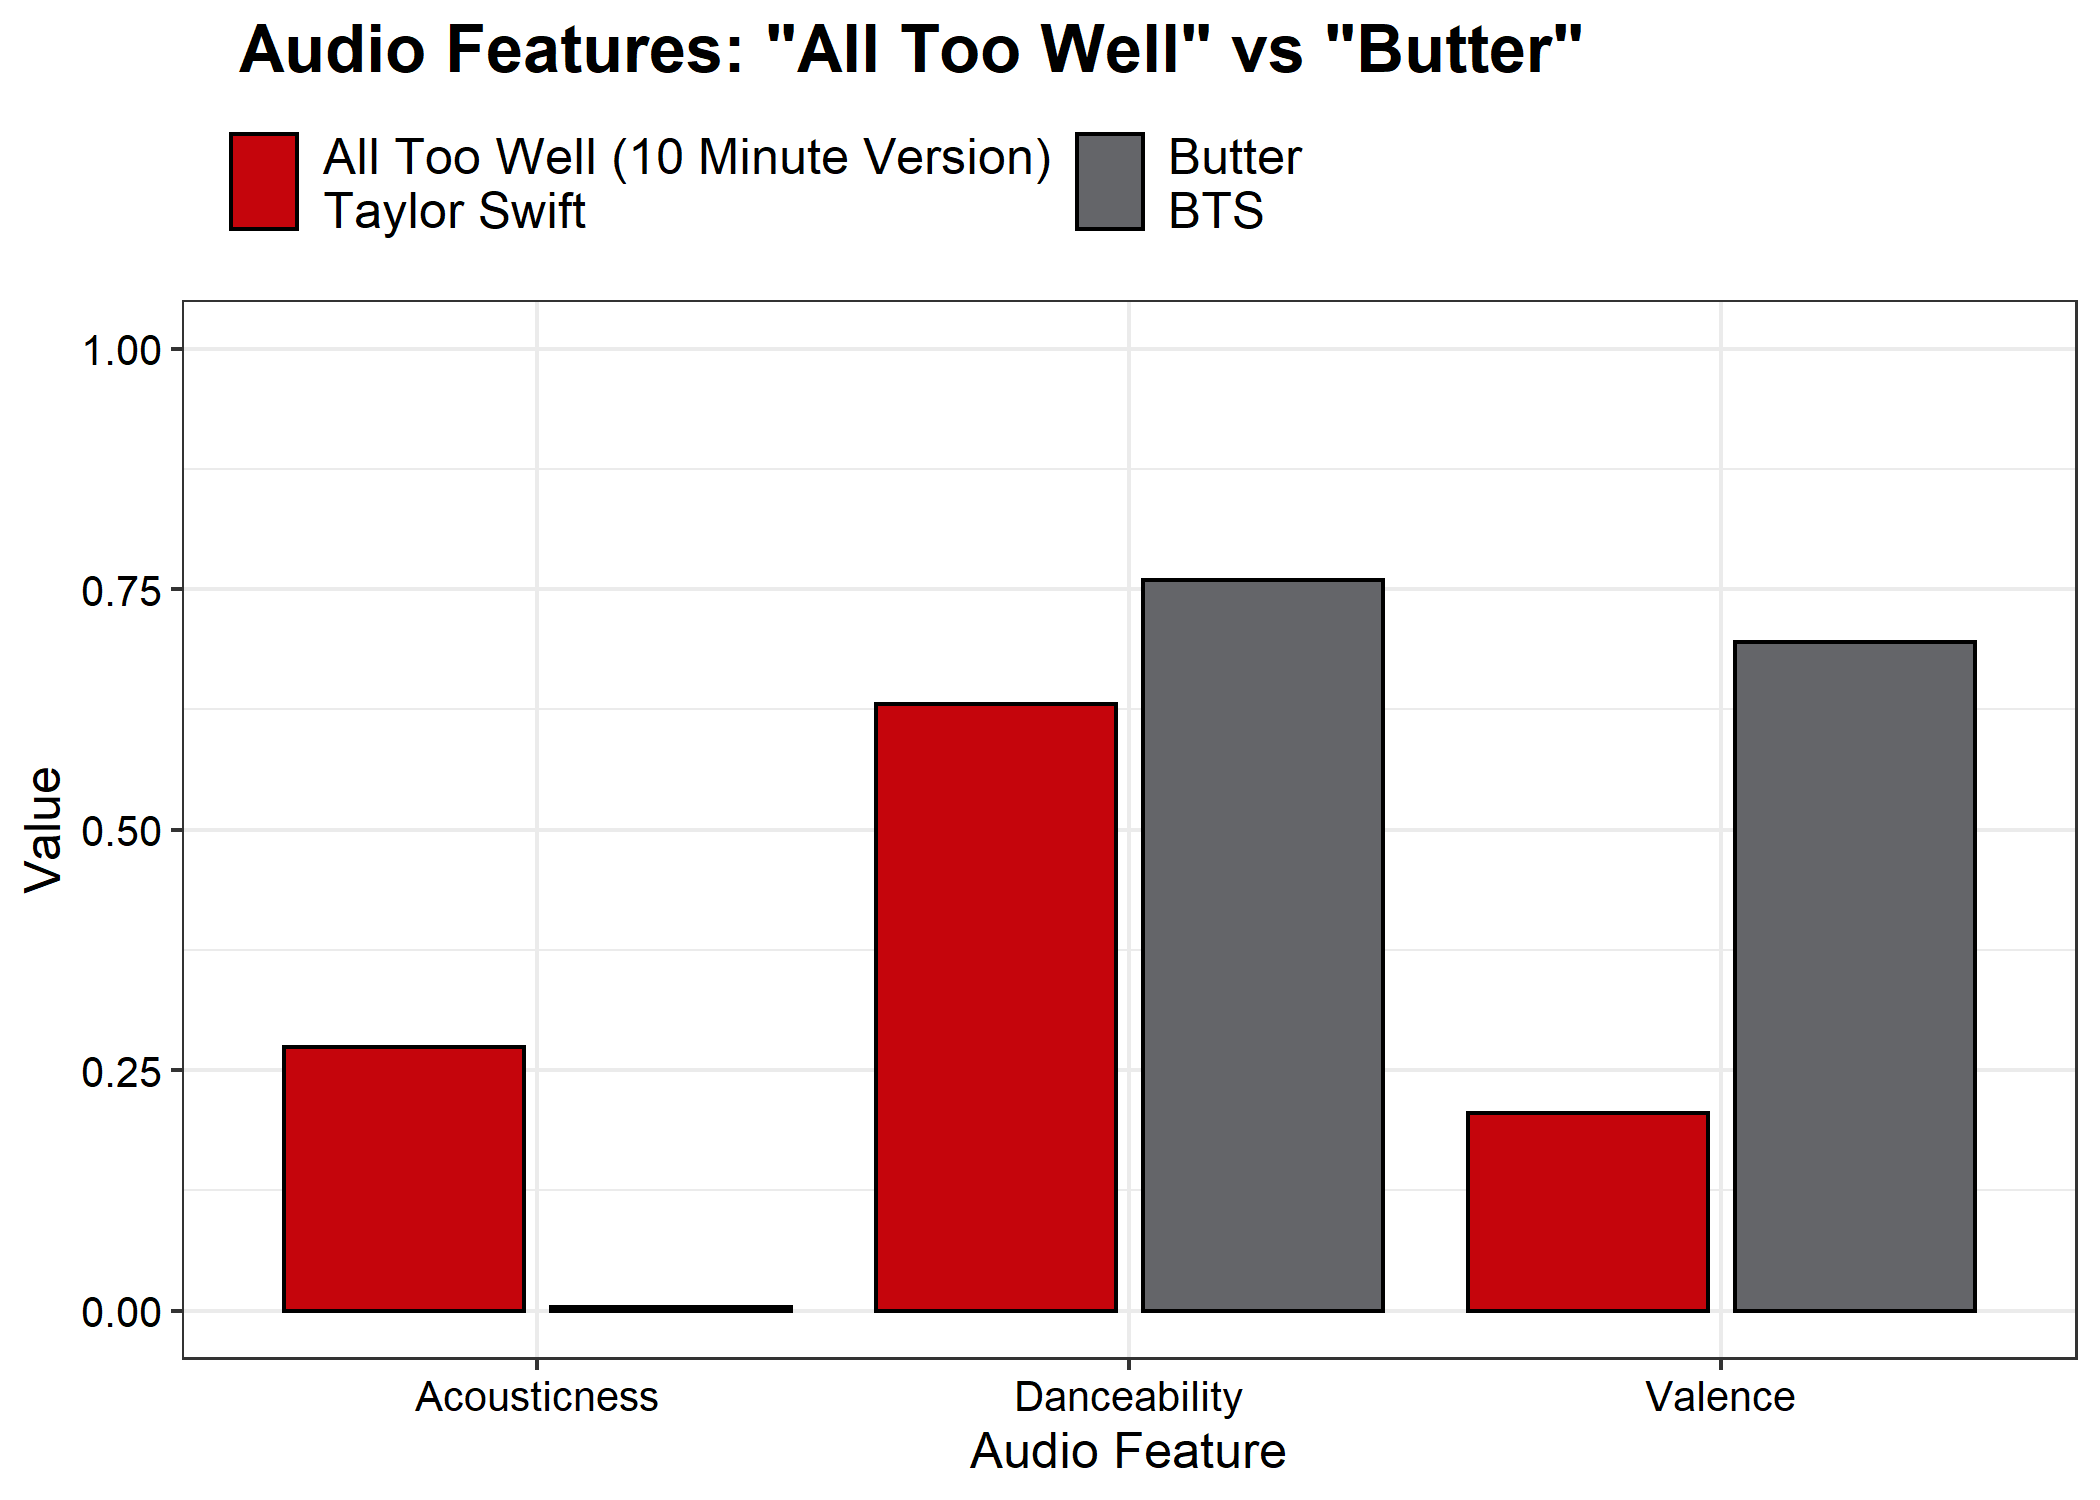
\includegraphics[width=0.7\textwidth]{alltoowell_v_butter.png}
\caption{Audio feature comparison between Taylor Swift's ``All Too Well" and BTS's ``Butter". The upbeat, buoyant vibe of ``Butter" leads to a much higher valence than ``All Too Well". Similarly, the complete lack of acoustic instrumentation in ``Butter" results in a near-zero acousticness score. Although we might expect ``Butter" to score radically higher on danceability than ``All Too Well", danceability is in fact comparable between songs (though ``Butter" does score slightly higher). Both have a steady, consistent beat and use little rhythmic fluctuation.}
\label{fig:alltoowell_vs_butter} 
\end{figure}

\subsection{Hierarchical Nature of the Data}
Songs within a certain period of time are likely to be correlated. Popular songs that were released in the 1970s, for instance, often share some characteristics. The same is true for other time periods. Similarly, since we are measuring present popularity of songs, rather than historic popularity, it may be the case that a listener's relationship with audio features could vary by time period. A listener may enjoy ``danceable" songs from the 1980s, but generally dislike more modern songs that score high in danceability (the converse, of course, may also be true for other listeners). It's for these reasons that I view the data through a hierarchical lens, using release decade as the grouping variable. In principle, a more narrow grouping (e.g., by year) could be employed. Since music is often conceptualized in a decade-by-decade fashion, decade is a natural grouping for the data.

\subsection{Exploration}
There is much to be learned about this dataset through visualization.

The below figure summarizes popularity by decade. Of course, popularity tends to be greater in more recent decades. This is simply reflective of the fact that we're measuring present popularity. In turn, it may also reflect Spotify's user demographics, since over 50\% of Spotify users are under the age of 34\footnote{\href{https://www.businessofapps.com/data/spotify-statistics/}{https://www.businessofapps.com/data/spotify-statistics/}}, and younger users will likely prefer newer songs. We also see that across all decades, the median popularity is greater than 50, and this is a product of having sampled generally popular songs, since songs were selected via the ``top hits" playlists. Finally, we observe there are many low-valued outliers within each decade---these observations will later prove particularly difficult to predict.

\begin{figure}[H] % H forces the figure to appear in this location, h! tries really hard to do the same thing
\centering
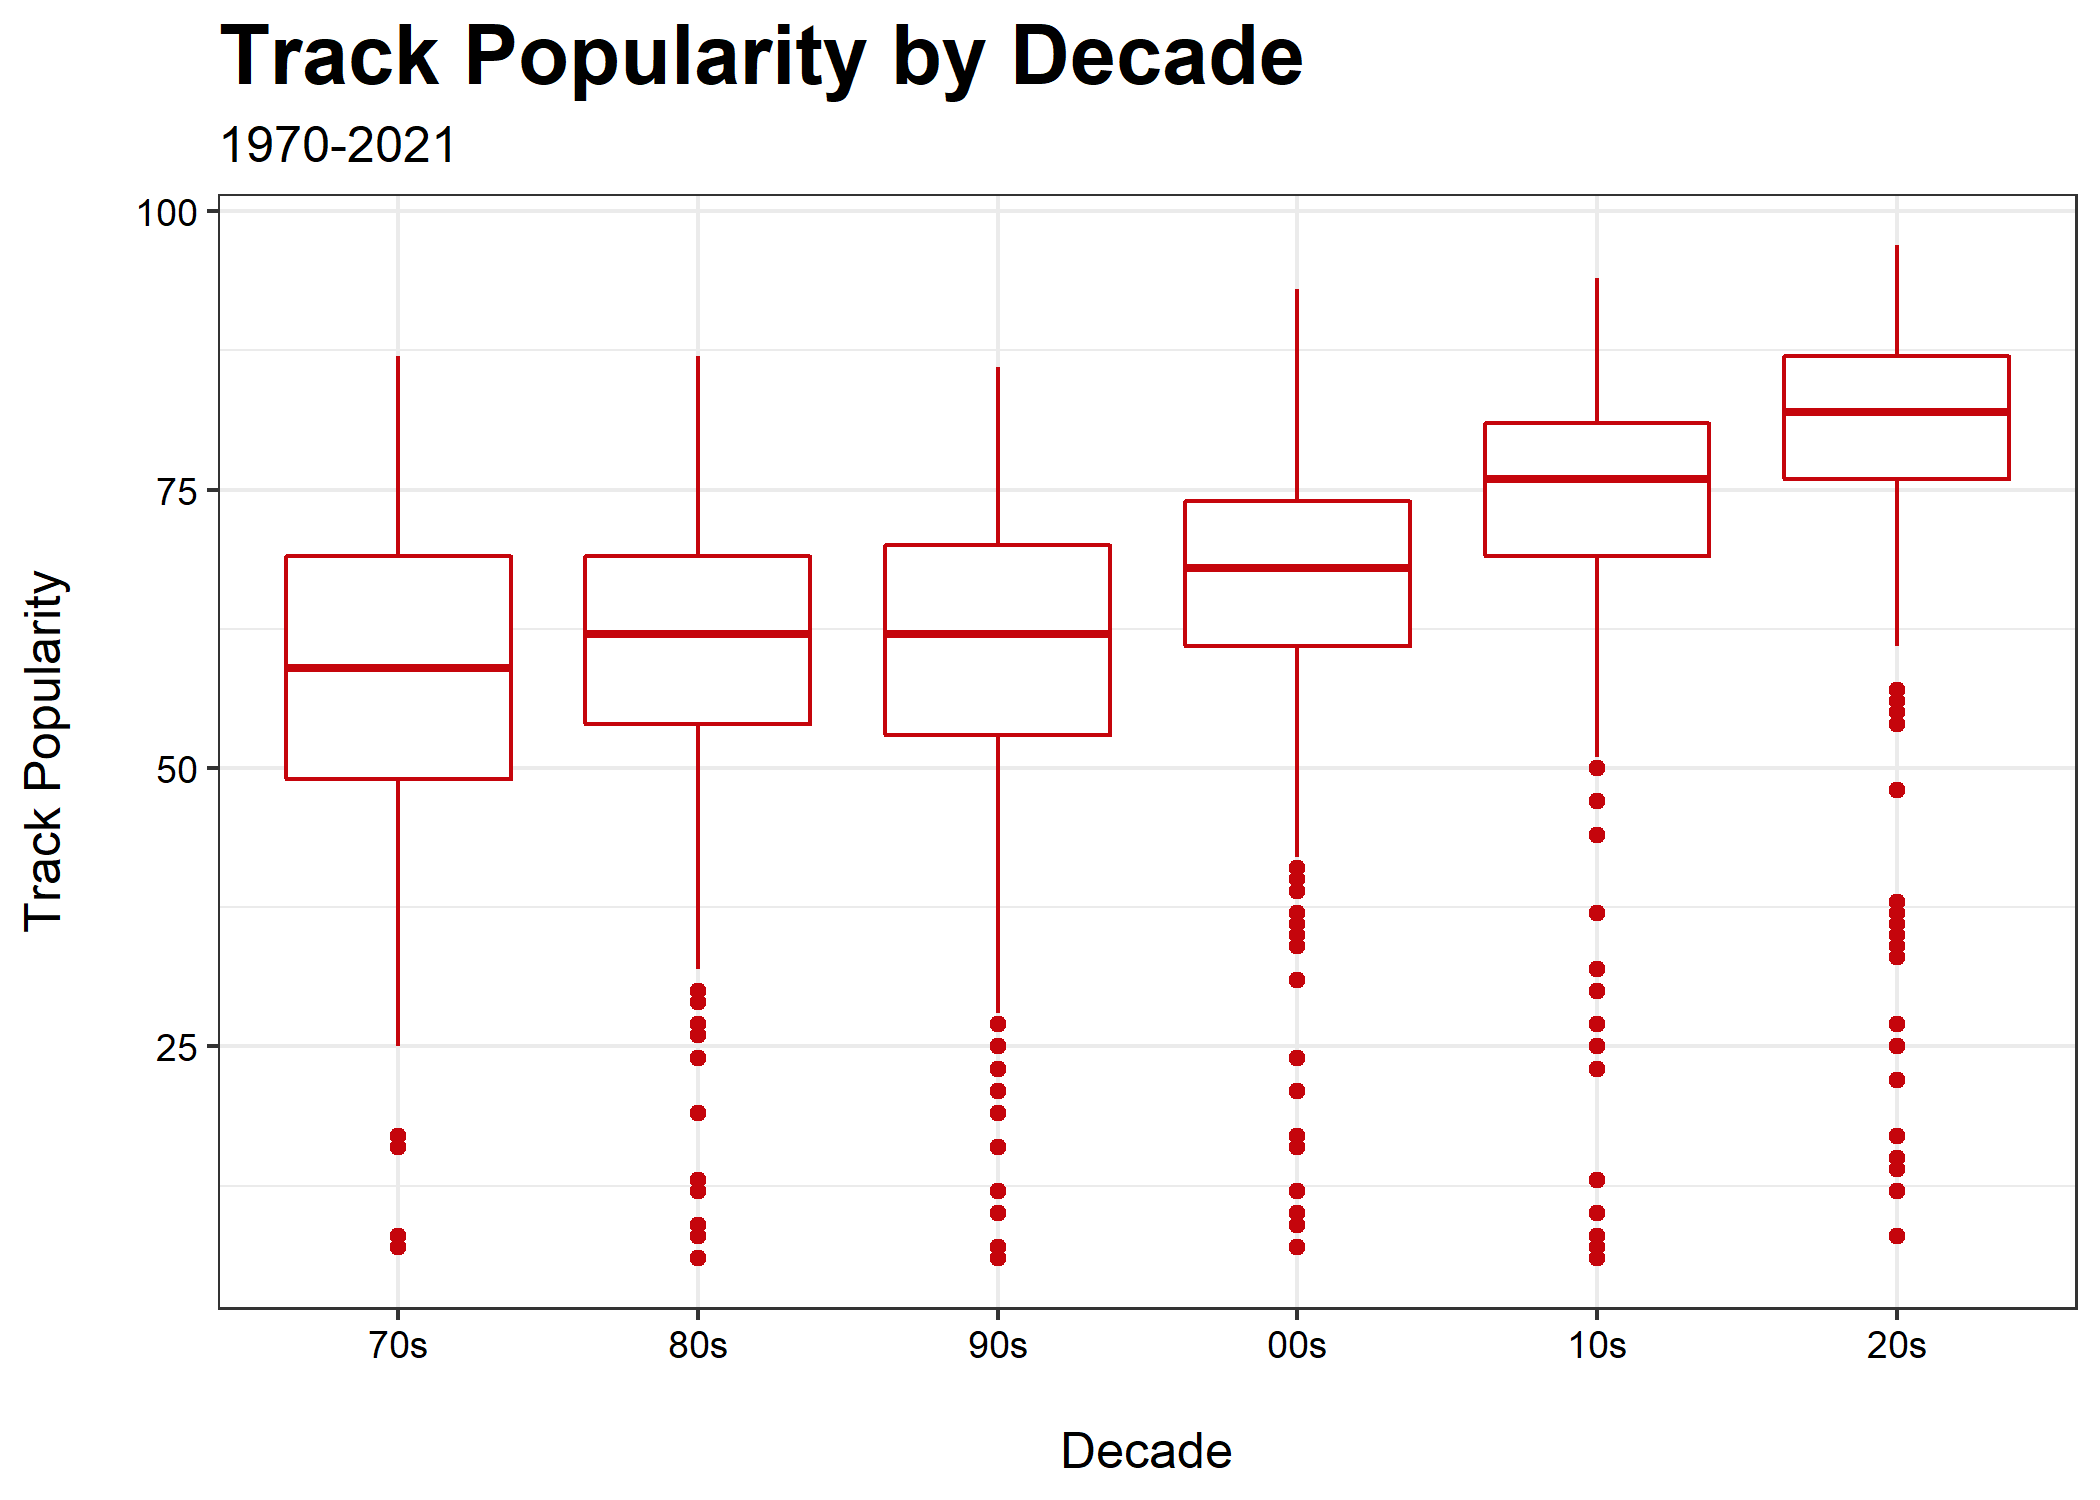
\includegraphics[width=0.7\textwidth]{track_pop_decade.png} % no need to specify a file extension & pay attention to scaling by width!
\caption{Track popularity over time. Since popularity is measuring present popularity, songs from more recent time periods have greater popularity. Note that ``20's" includes only 2020 and 2021.}
\label{fig:track_pop_decade} % useful for hyperref'ing later
\end{figure}

There are other interesting temporal features of this dataset. In particular, there are prominent trends among some of the predictors:

\begin{figure}[H]
\begin{subfigure}[b]{0.5\textwidth}
\centering
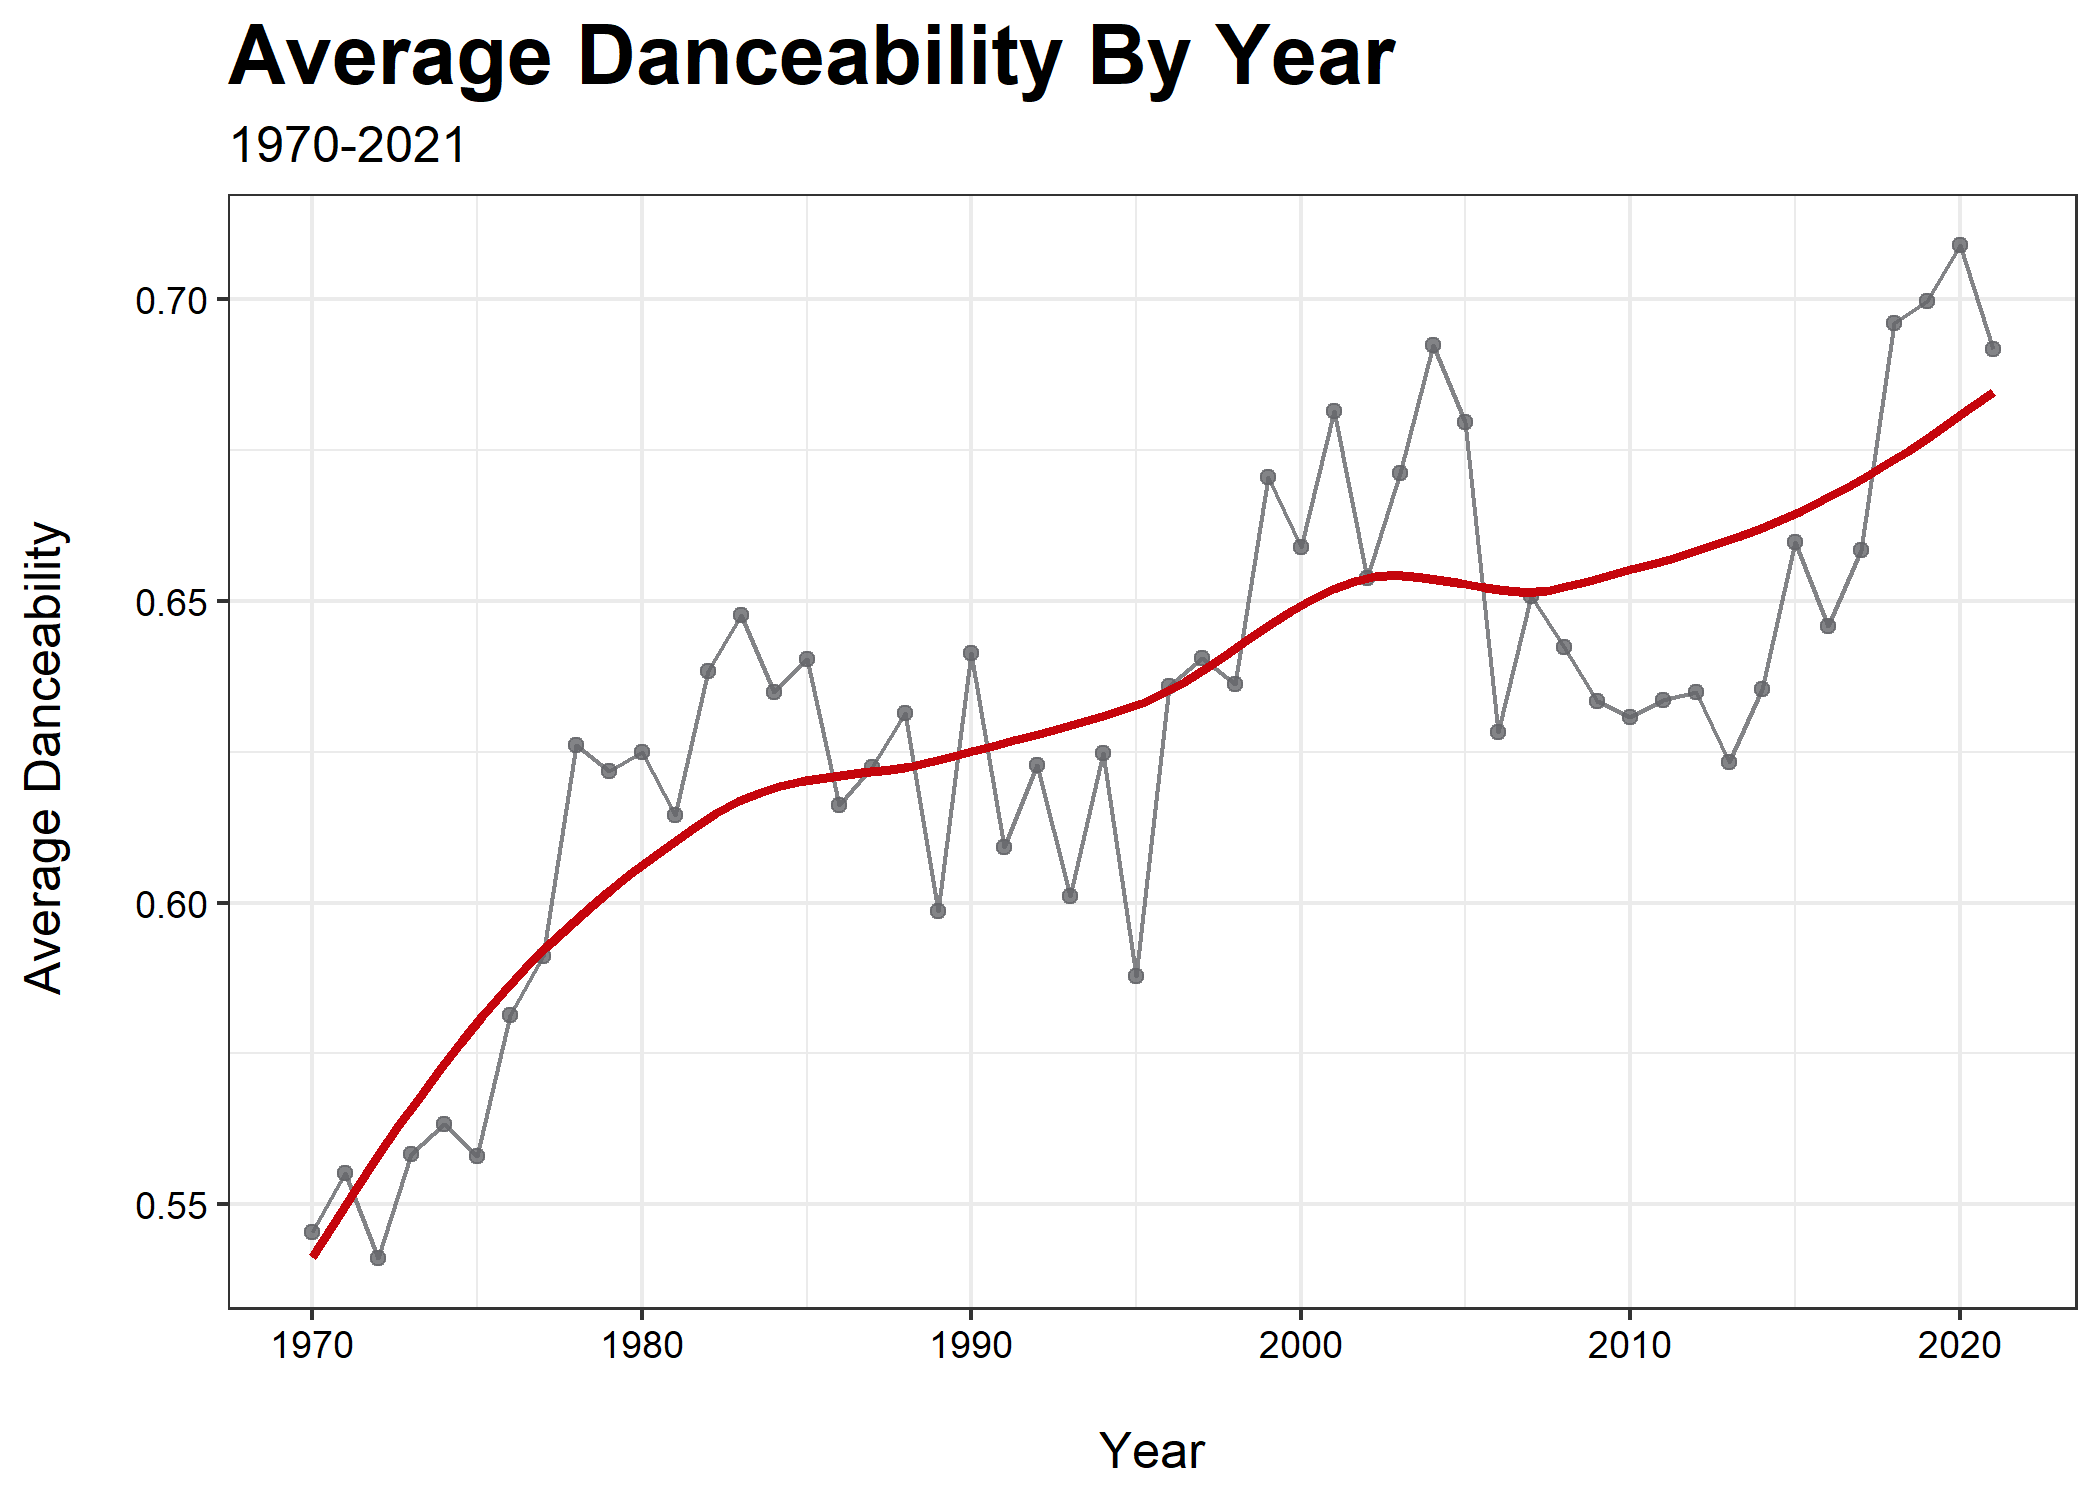
\includegraphics[width = \textwidth]{track_danceability_trend_.png}
\caption{}
\label{fig:danceability_trend}
\end{subfigure}
\begin{subfigure}[b]{0.5\textwidth}
\centering
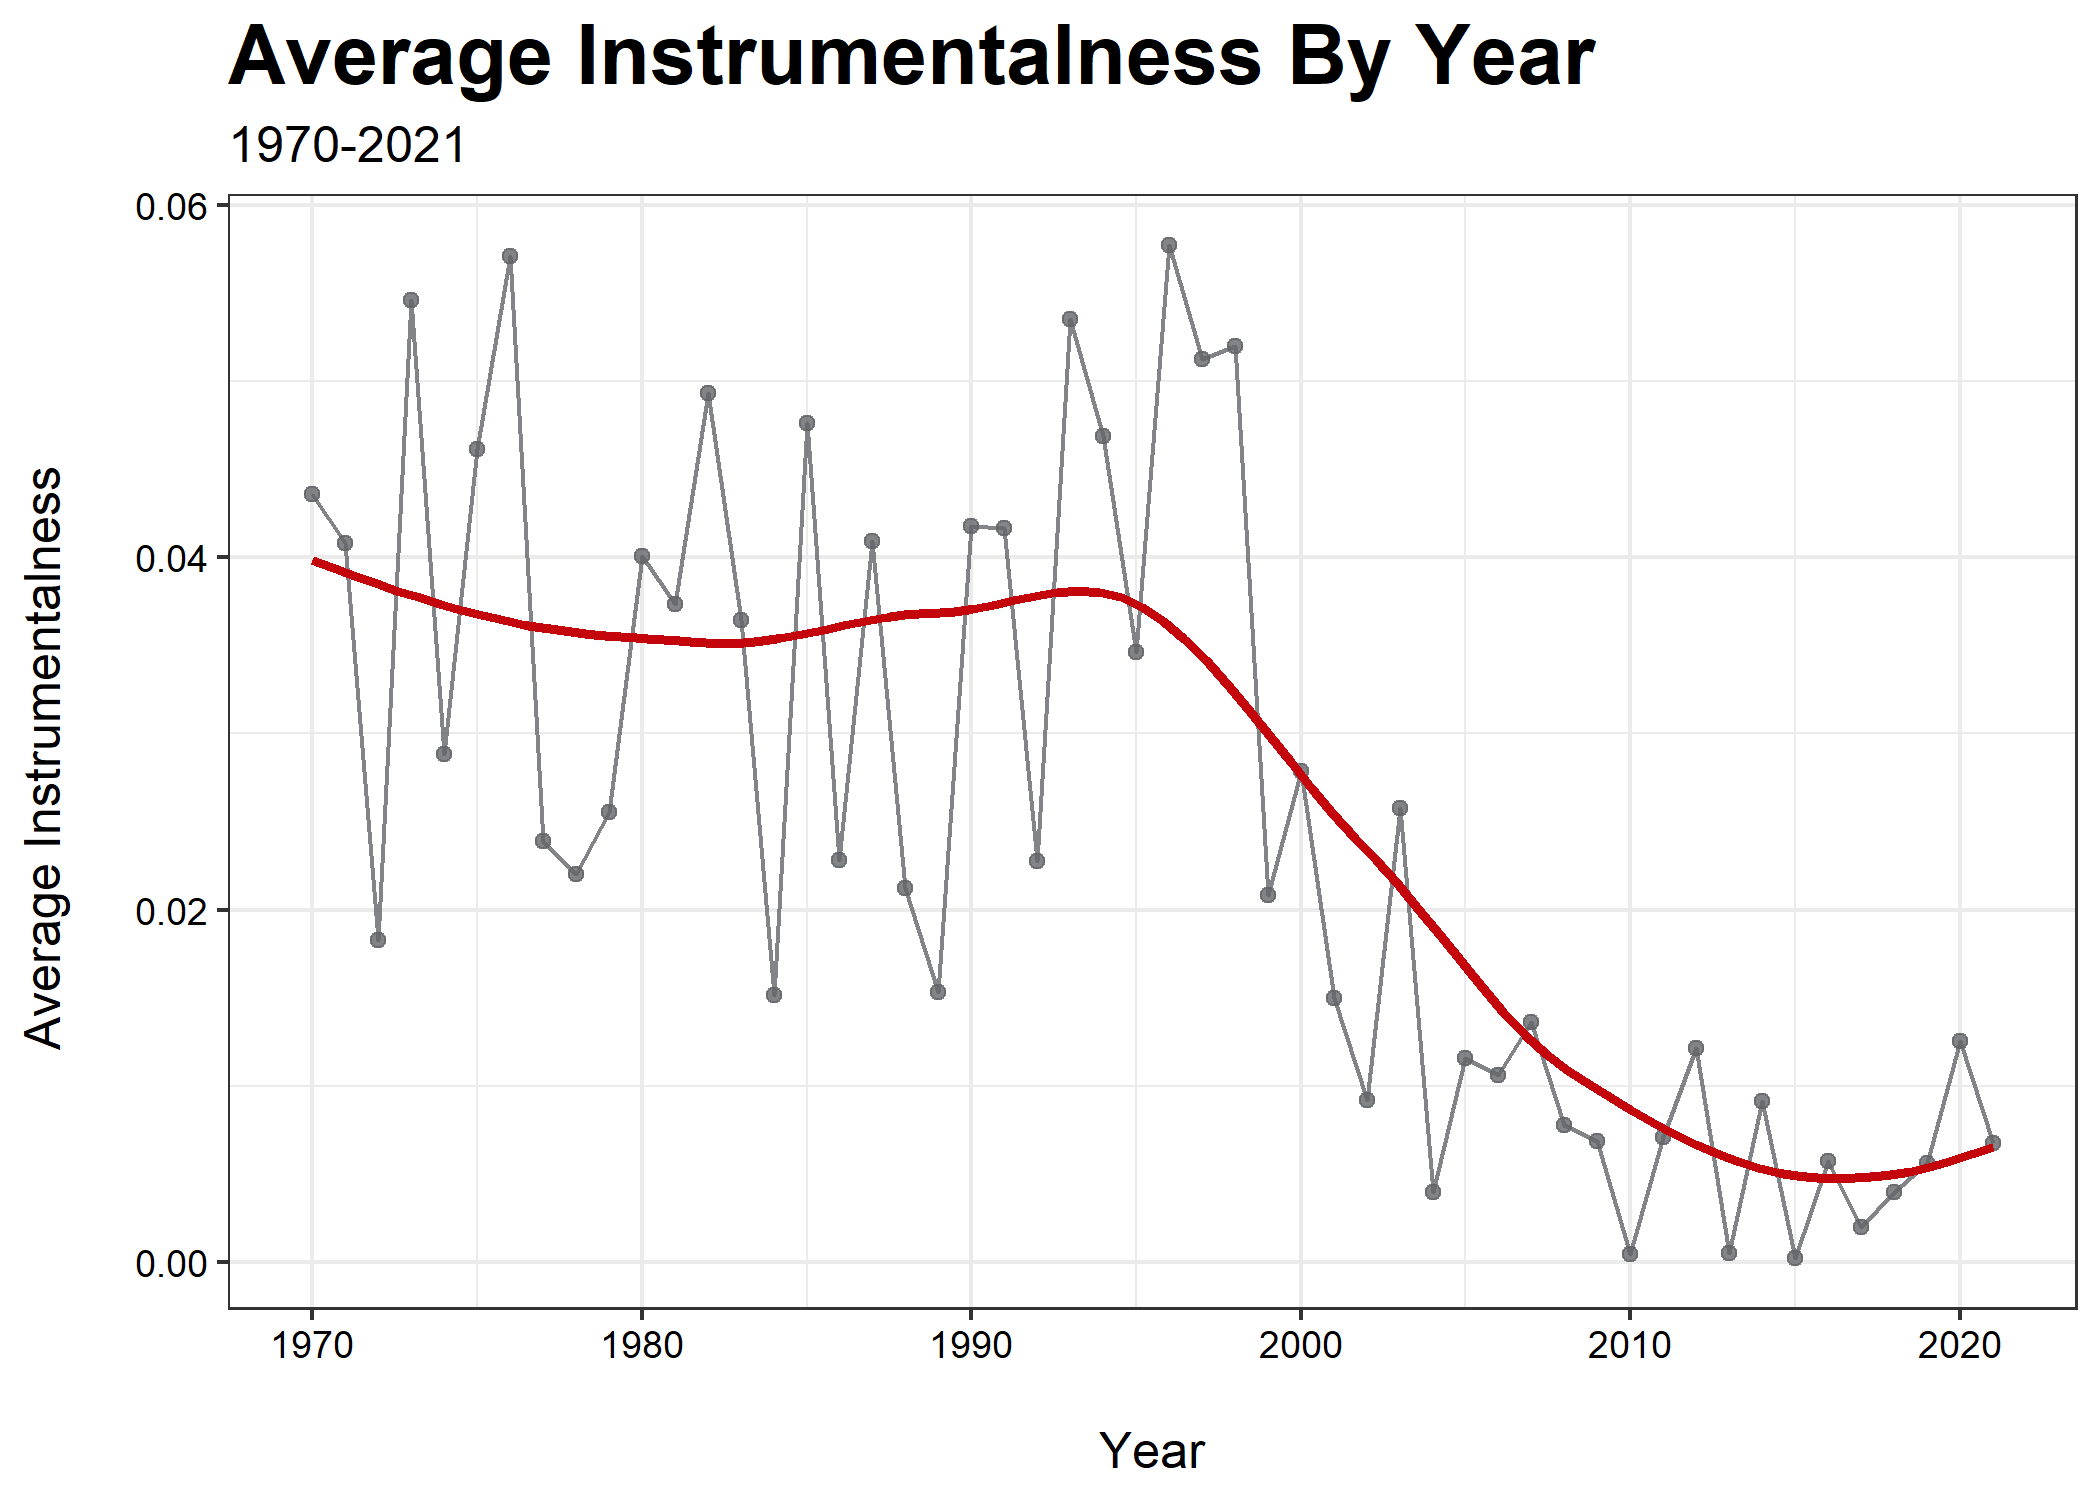
\includegraphics[width = \textwidth]{track_instrumentalness_trend_.png}
\caption{}
\label{fig:instrumentalness_trend}
\end{subfigure}
\begin{subfigure}[b]{0.5\textwidth}
\centering
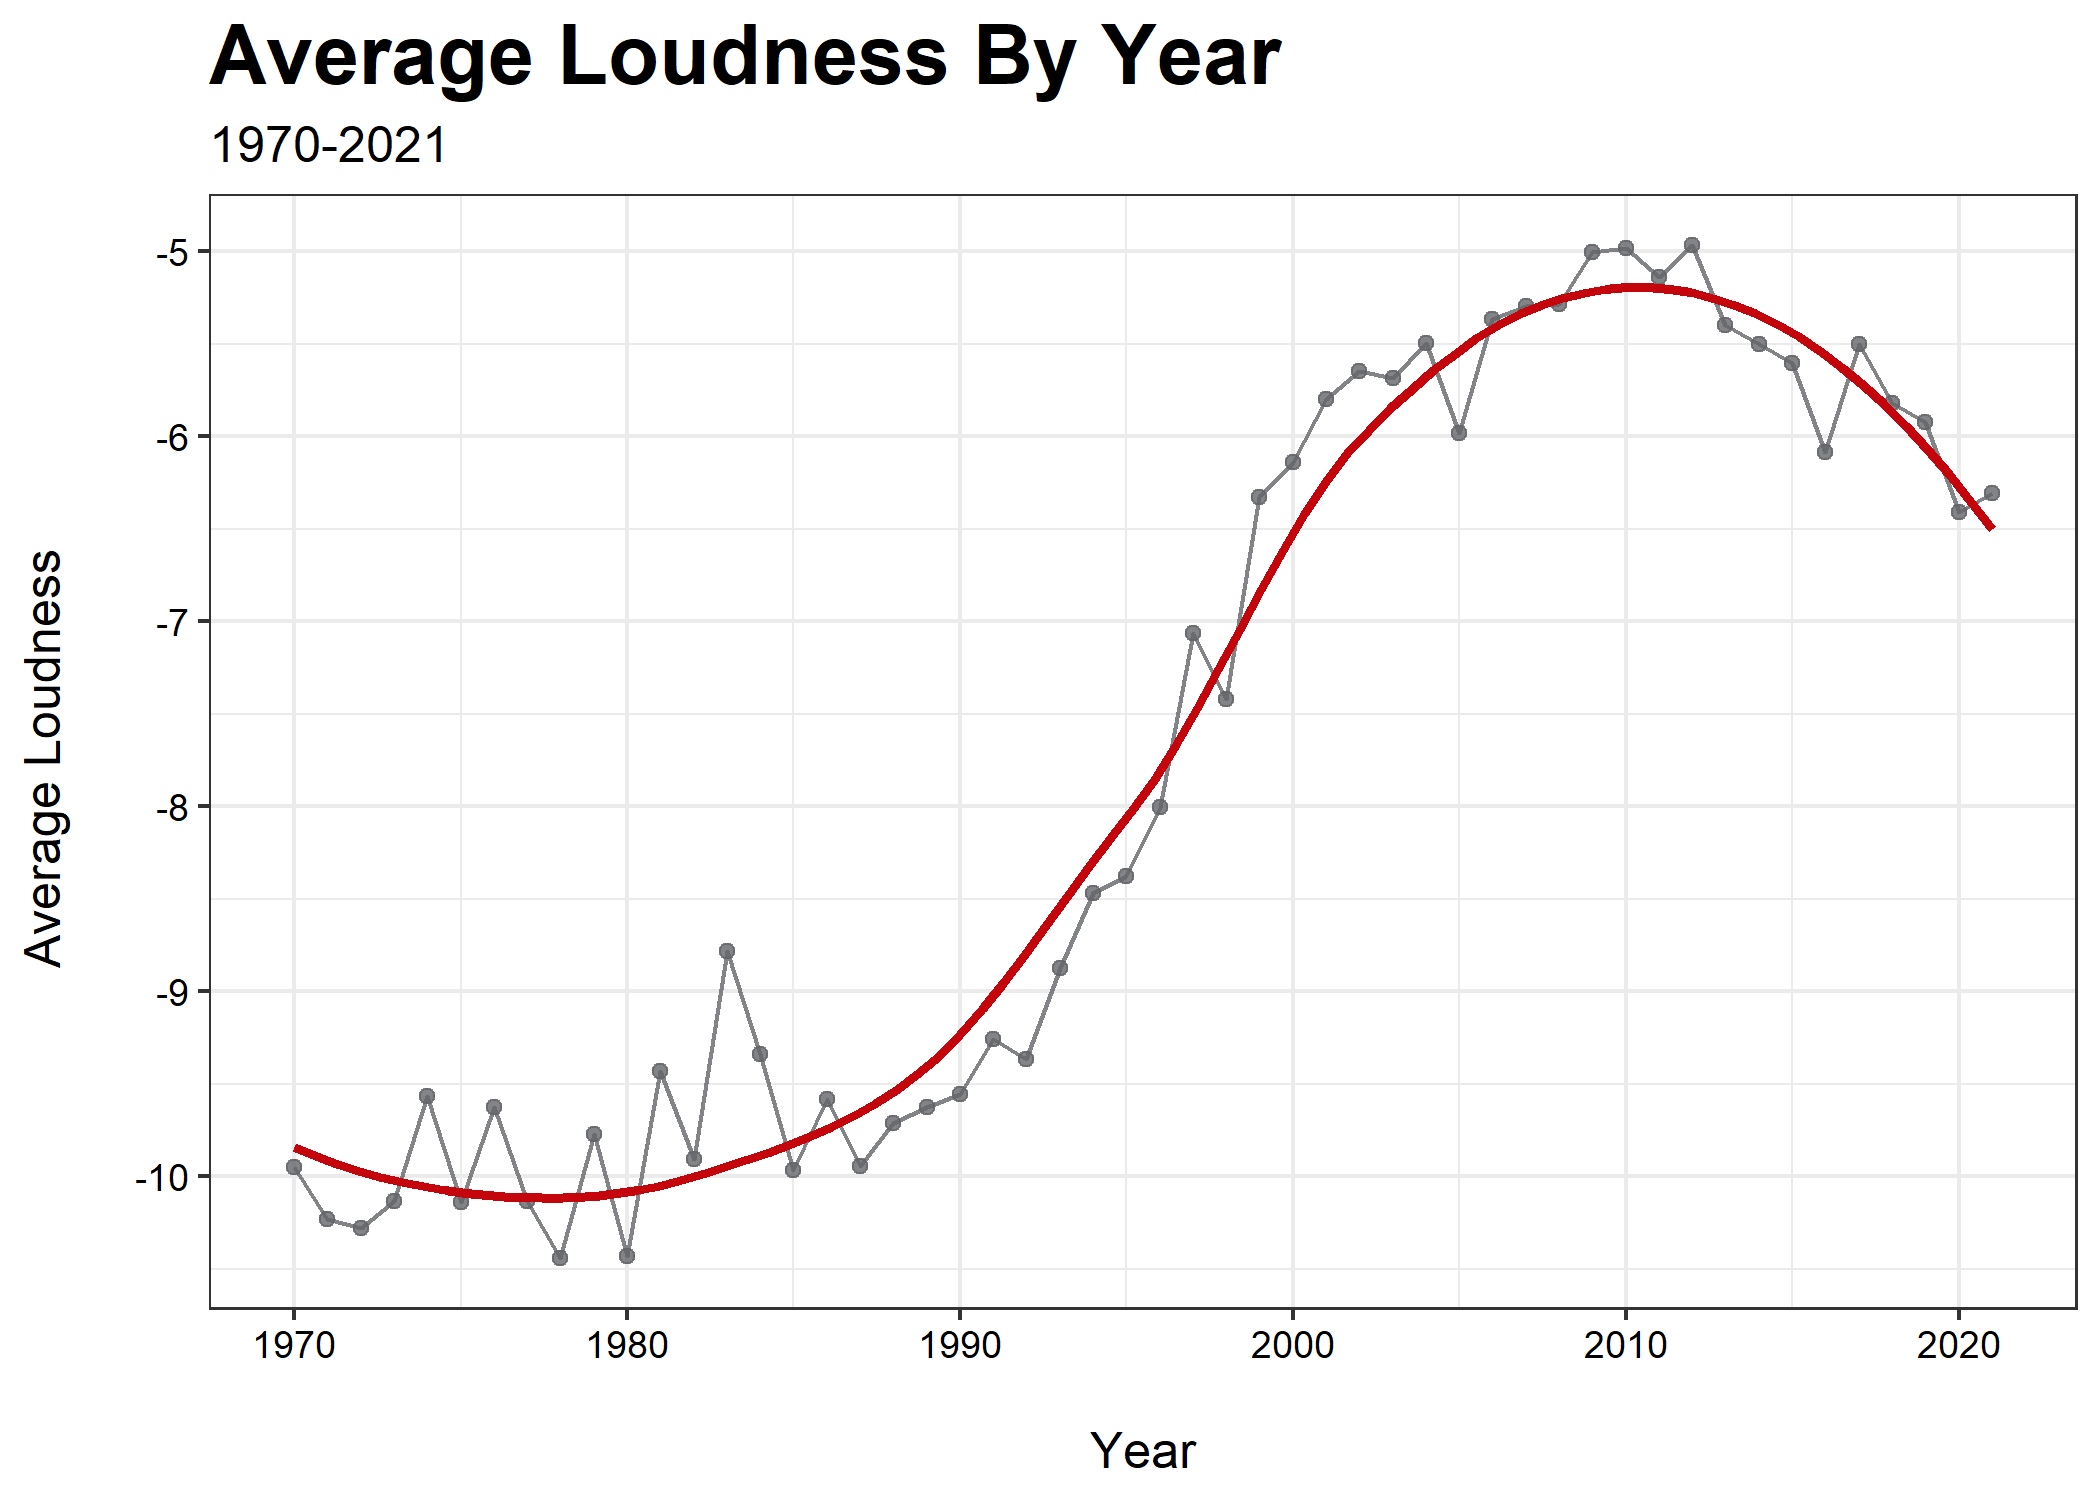
\includegraphics[width = \textwidth]{track_loudness_trend_.png}
\caption{}
\label{fig:loudness_trend}
\end{subfigure}
\begin{subfigure}[b]{0.5\textwidth}
\centering
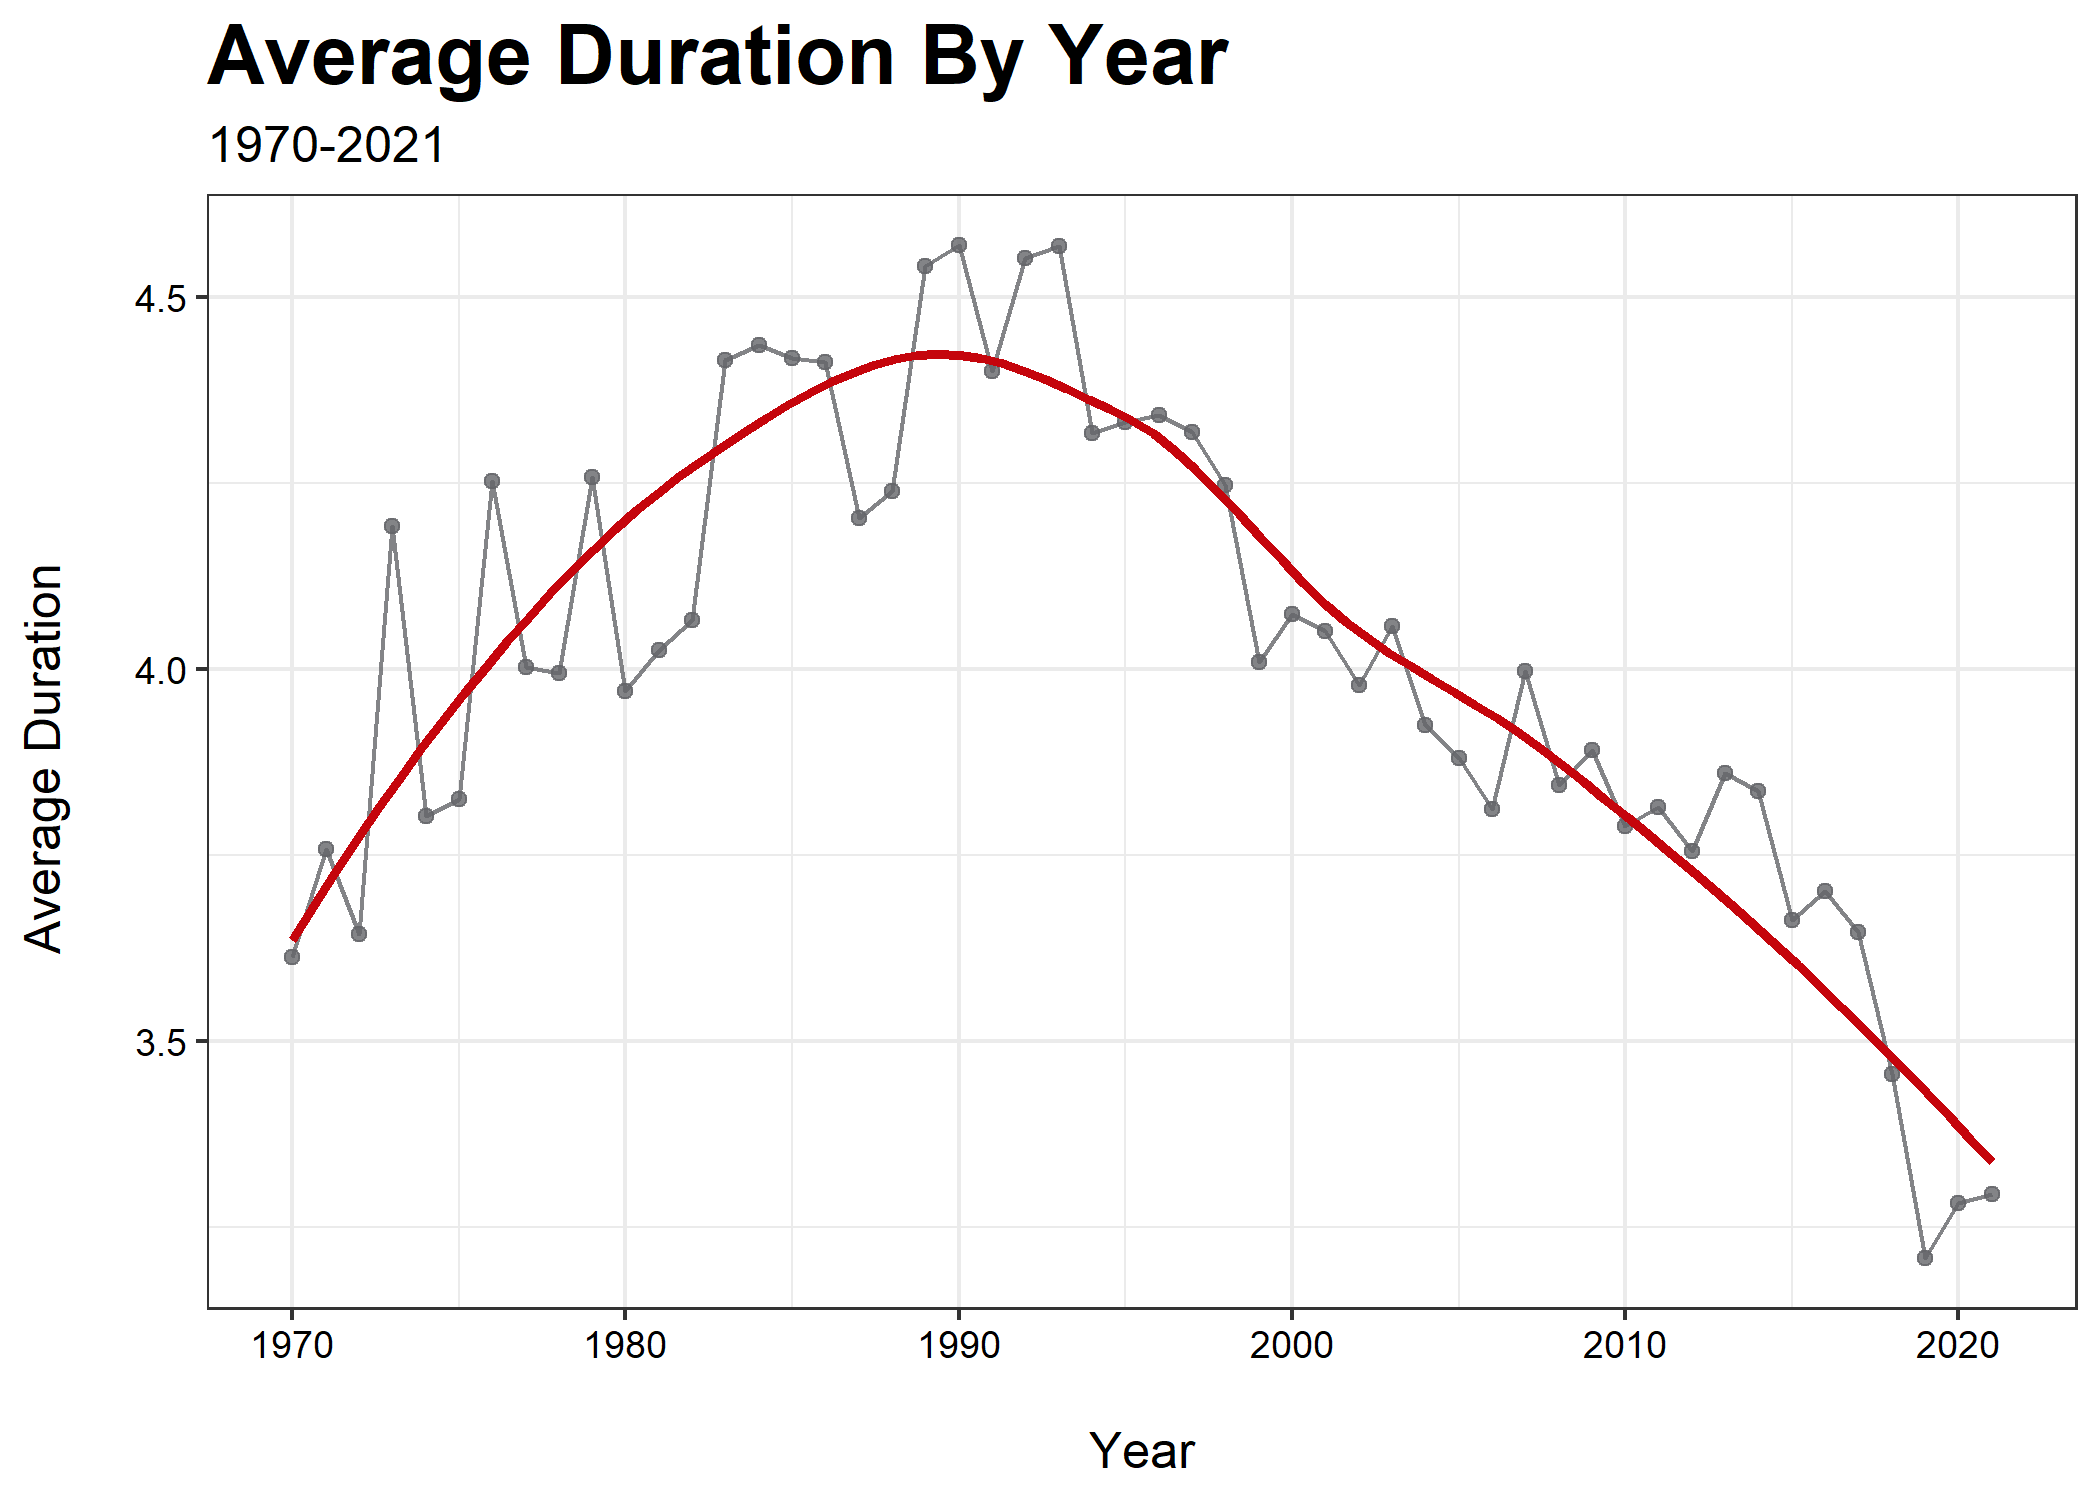
\includegraphics[width = \textwidth]{track_duration_trend_.png}
\caption{}
\label{fig:duration_trend}
\end{subfigure}
\caption{Trends in danceability, instrumnetalness, loudness, and duration metrics by year. Popular songs were, on average, getting louder and louder from about 1990 up until around 2010. We also observe a sharp decline in average instrumentalness around 1995. These figures also highlight the importance of considering temporal correlation within the data---songs within particularly periods of time are, on average, similar in their audio features.}
\label{fig:multipart_figure}
\end{figure}
% Further, it's not surprising that there is some apparent colinearity among the predictors. Intuitively, we'd expect songs high in acousticness to also score low in loudness, for example.

% \begin{figure}[H] % H forces the figure to appear in this location, h! tries really hard to do the same thing
% \centering
% 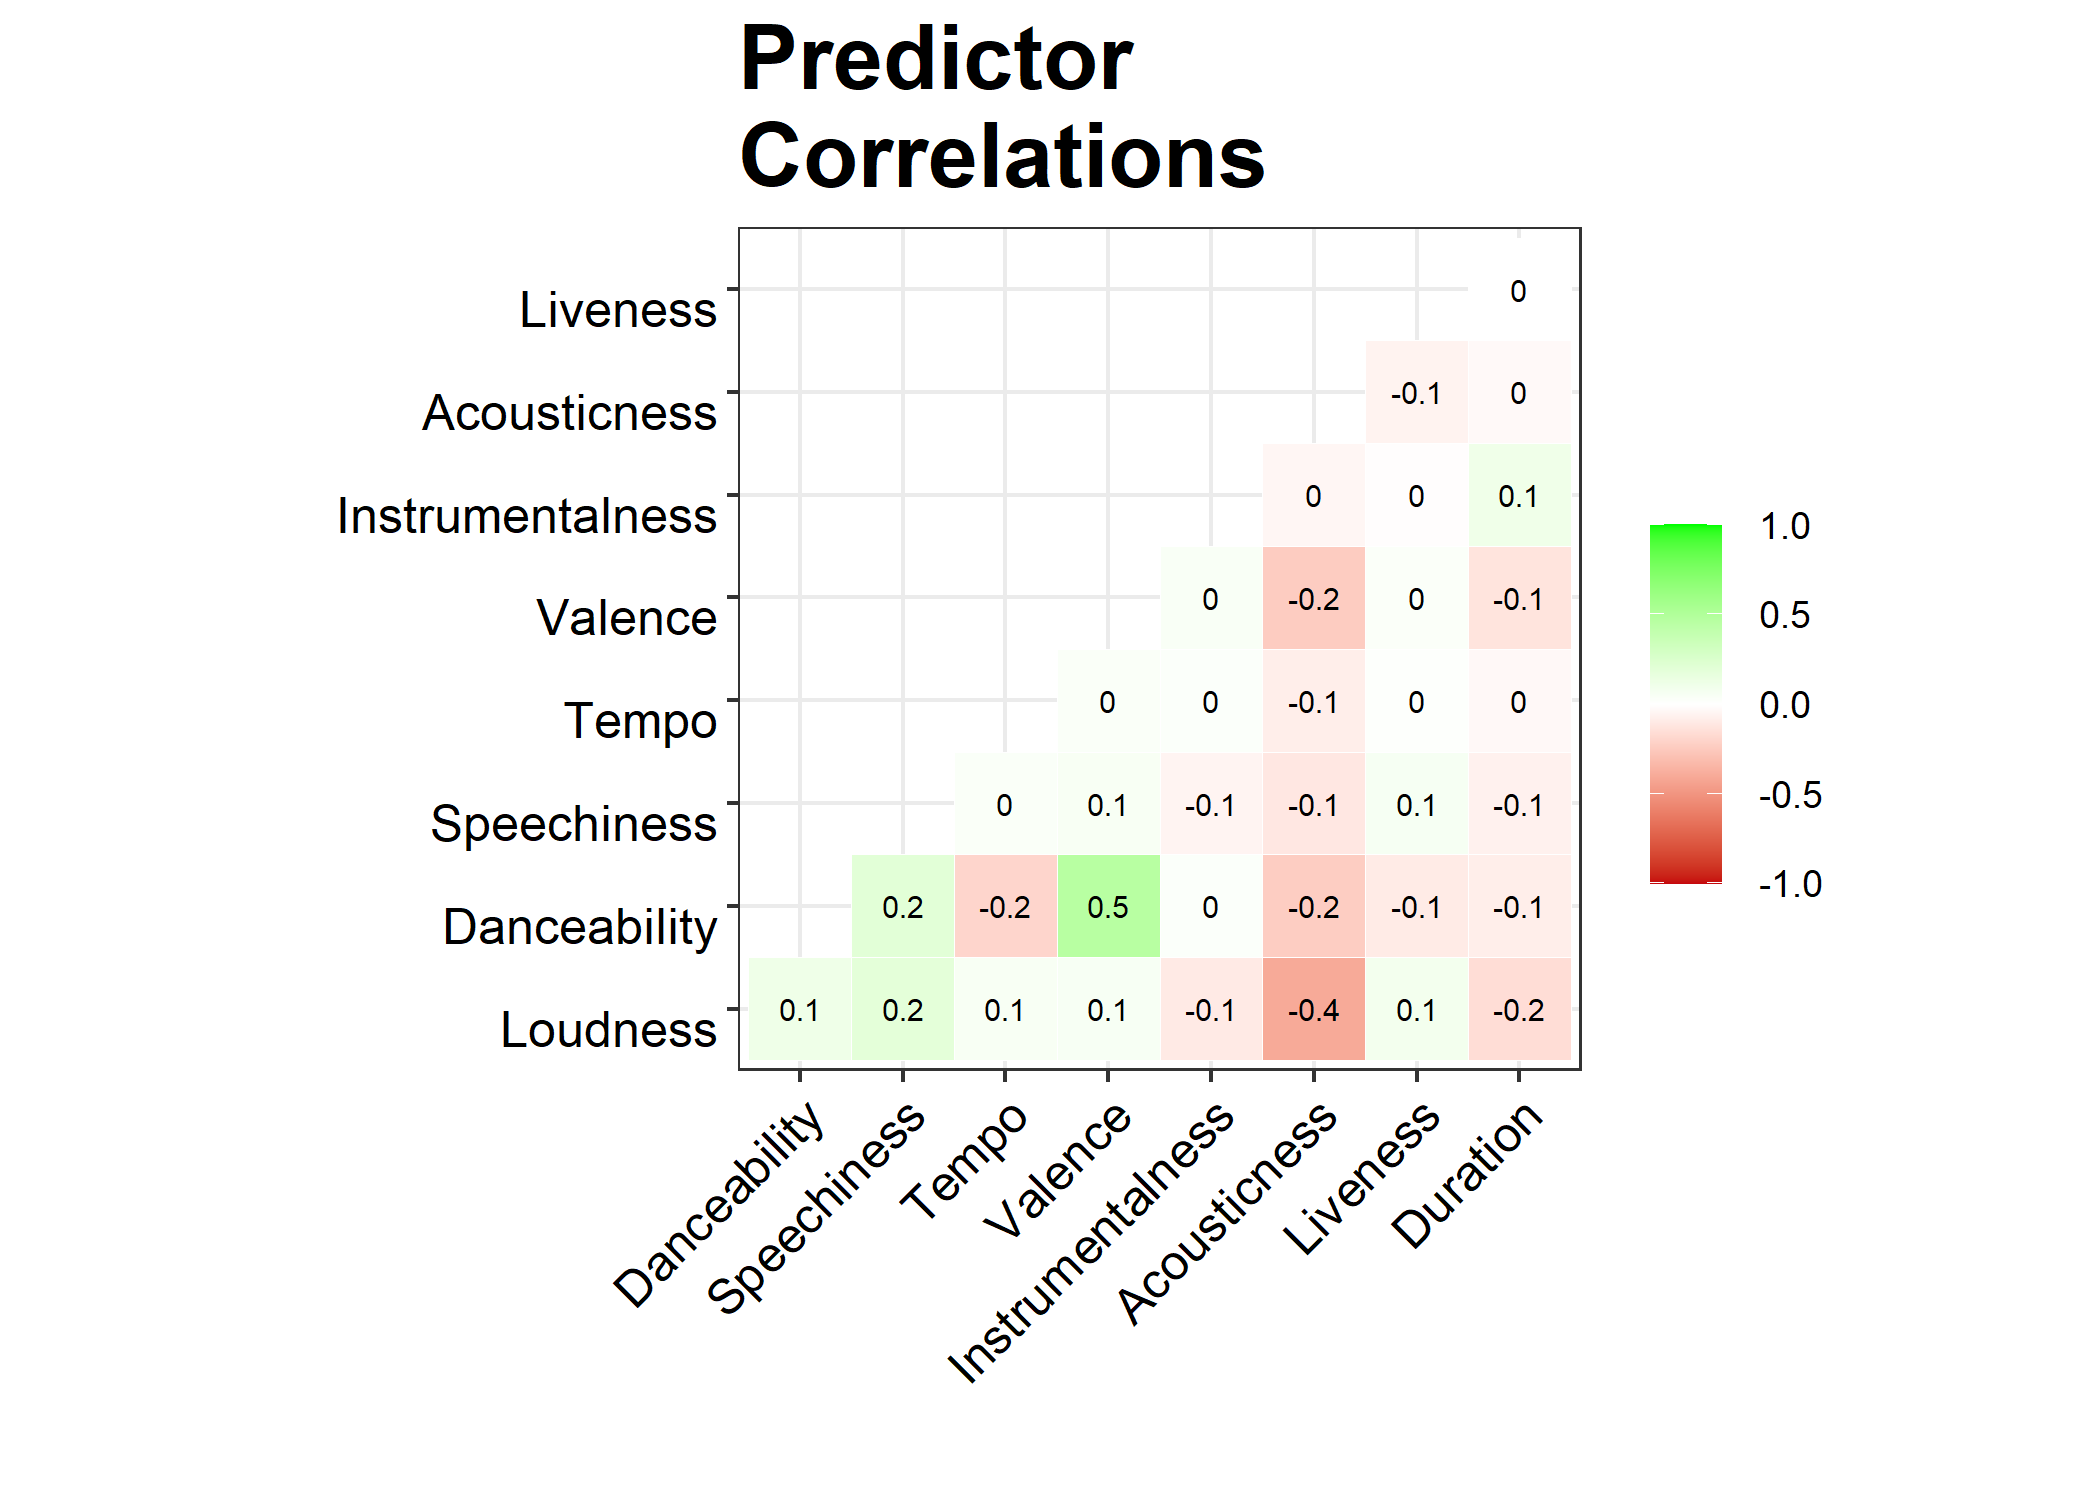
\includegraphics[width=1\textwidth]{predictor_correlations.png} % no need to specify a file extension & pay attention to scaling by width!
% \caption{}
% \label{fig:predictor_cor} % useful for hyperref'ing later
% \end{figure}
In addition to the 9 audio features described in Table \ref{table:audio_features}, artist popularity is also considered. As one would expect, this predictor simply measures the overall popularity of a song's artist. Artist popularity is used, in some sense, as a control variable. We ultimately aim to understand the predictive relationship between song popularity and audio features, but it seems likely that some artists could reach such a high level of fame and recognition that their songs become popular independently from their audio features. We will therefor allow artist popularity to enter the model, serving as a type of control.

Further, the ``energy" feature was omitted from consideration due to reasonably high colinearity with several other features. In particular, its correlation coefficient with loudness, acousticness, and valence was 0.70, -0.60, and 0.40, respectively. 

Visual inspection suggests that the relationships between song popularity and each of the 10 predictors in consideration are surprisingly weak:

\begin{figure}[H]
\begin{subfigure}[b]{0.5\textwidth}
\centering
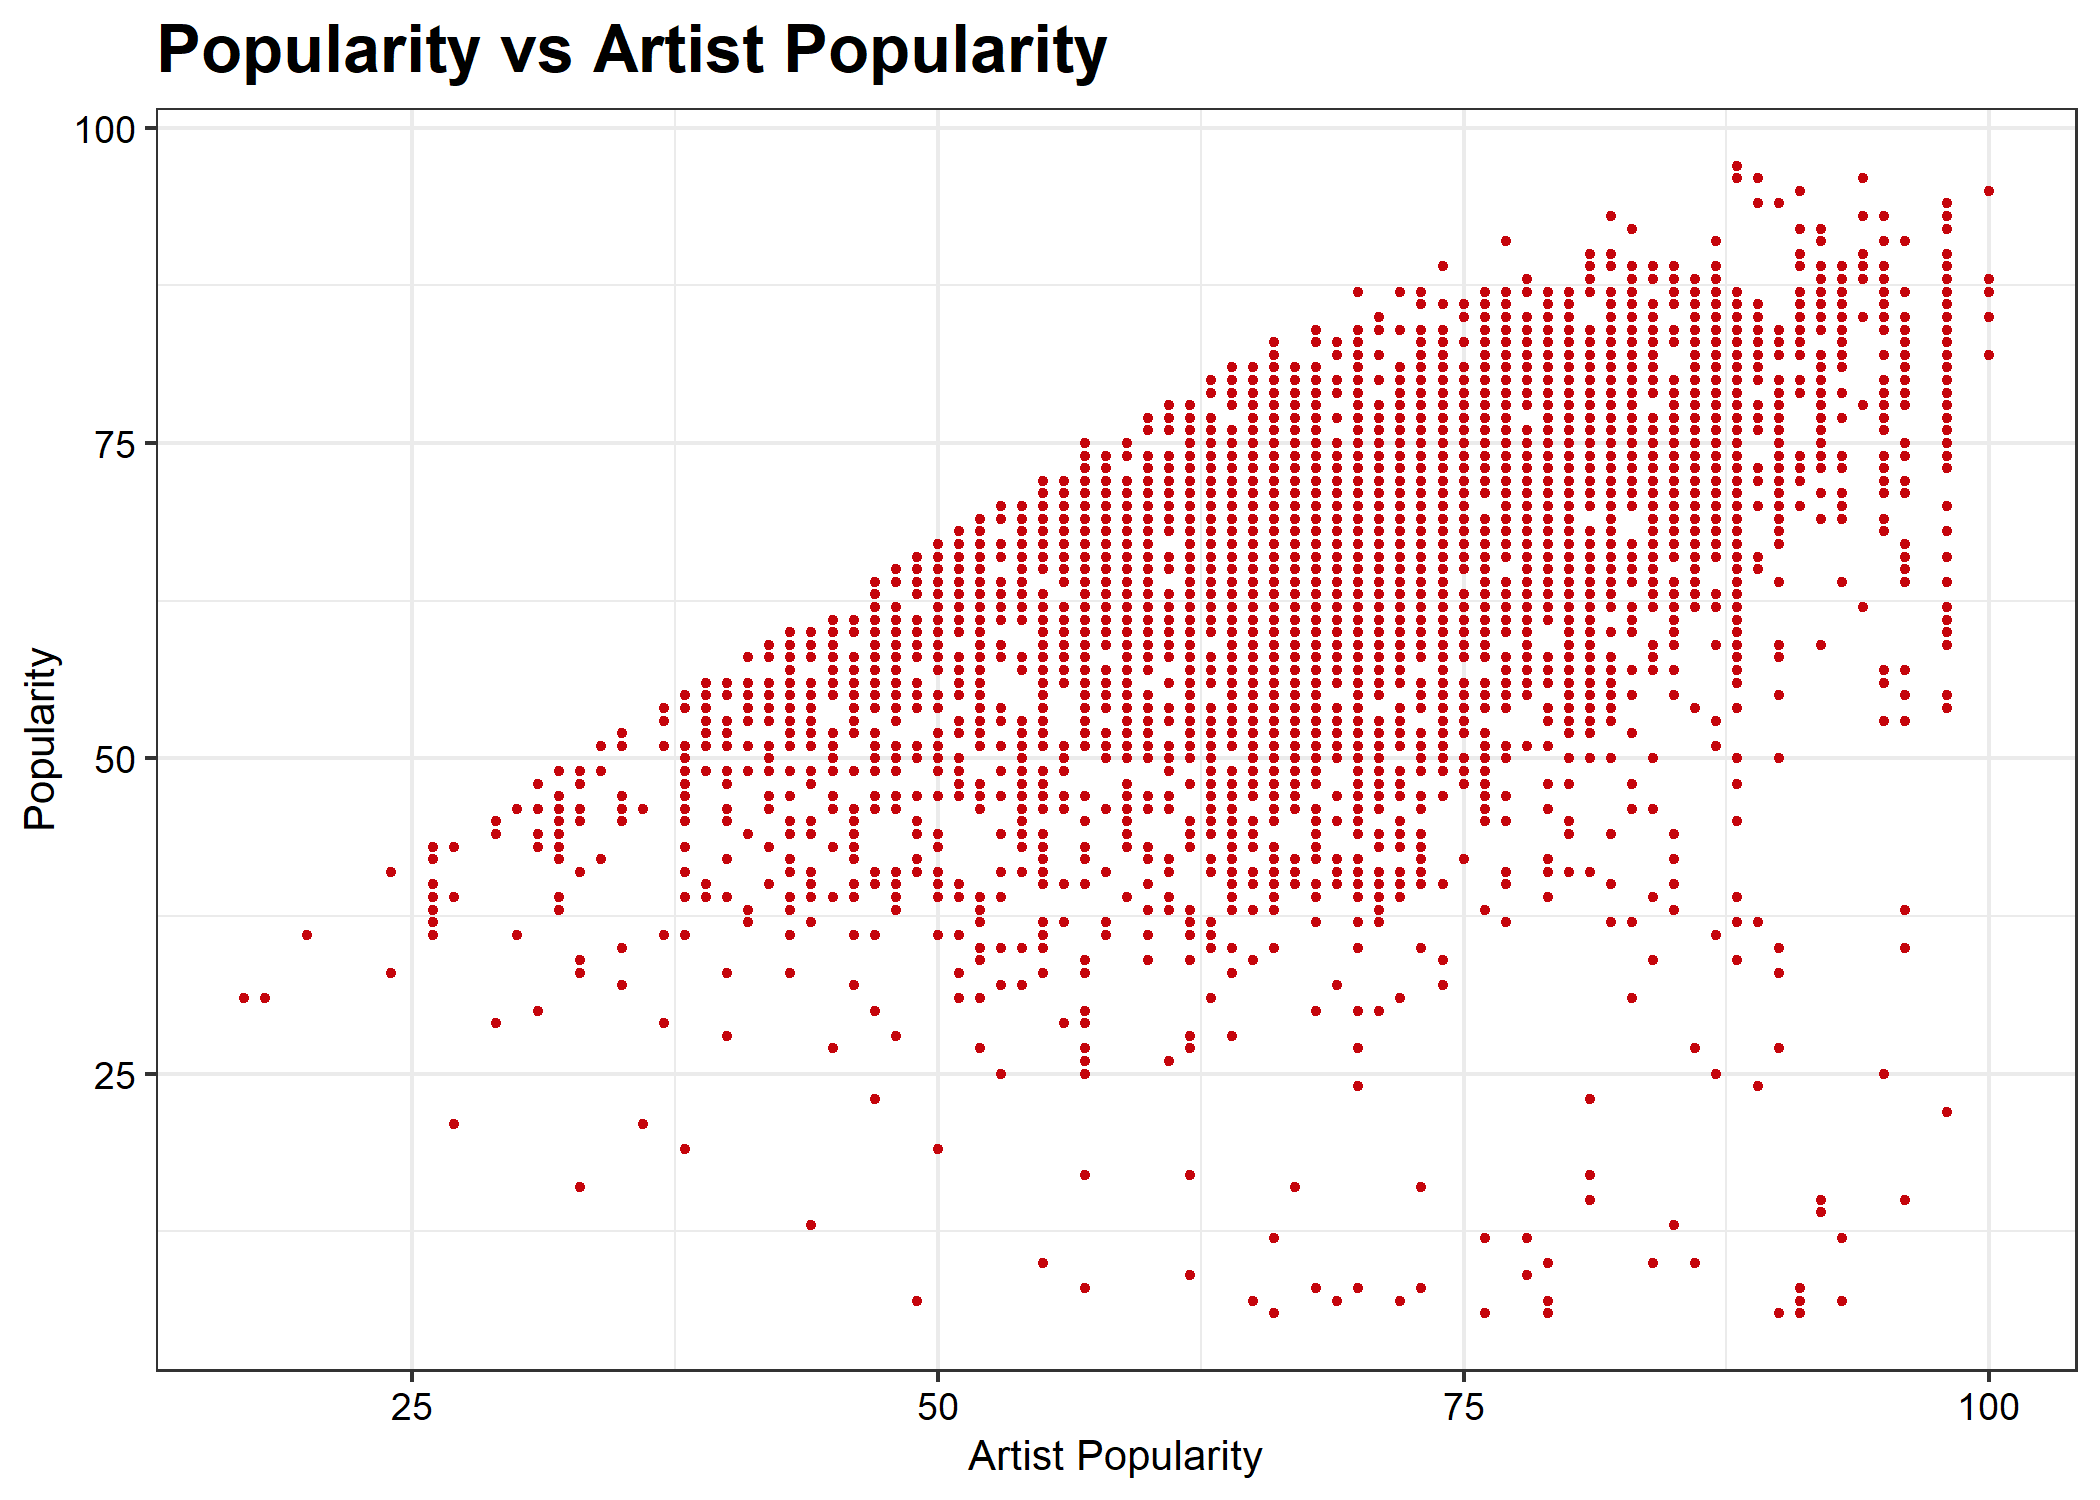
\includegraphics[width = \textwidth]{pop_vs_artist_pop.png}
\caption{}
\label{fig:danceability_trend}
\end{subfigure}
\begin{subfigure}[b]{0.5\textwidth}
\centering
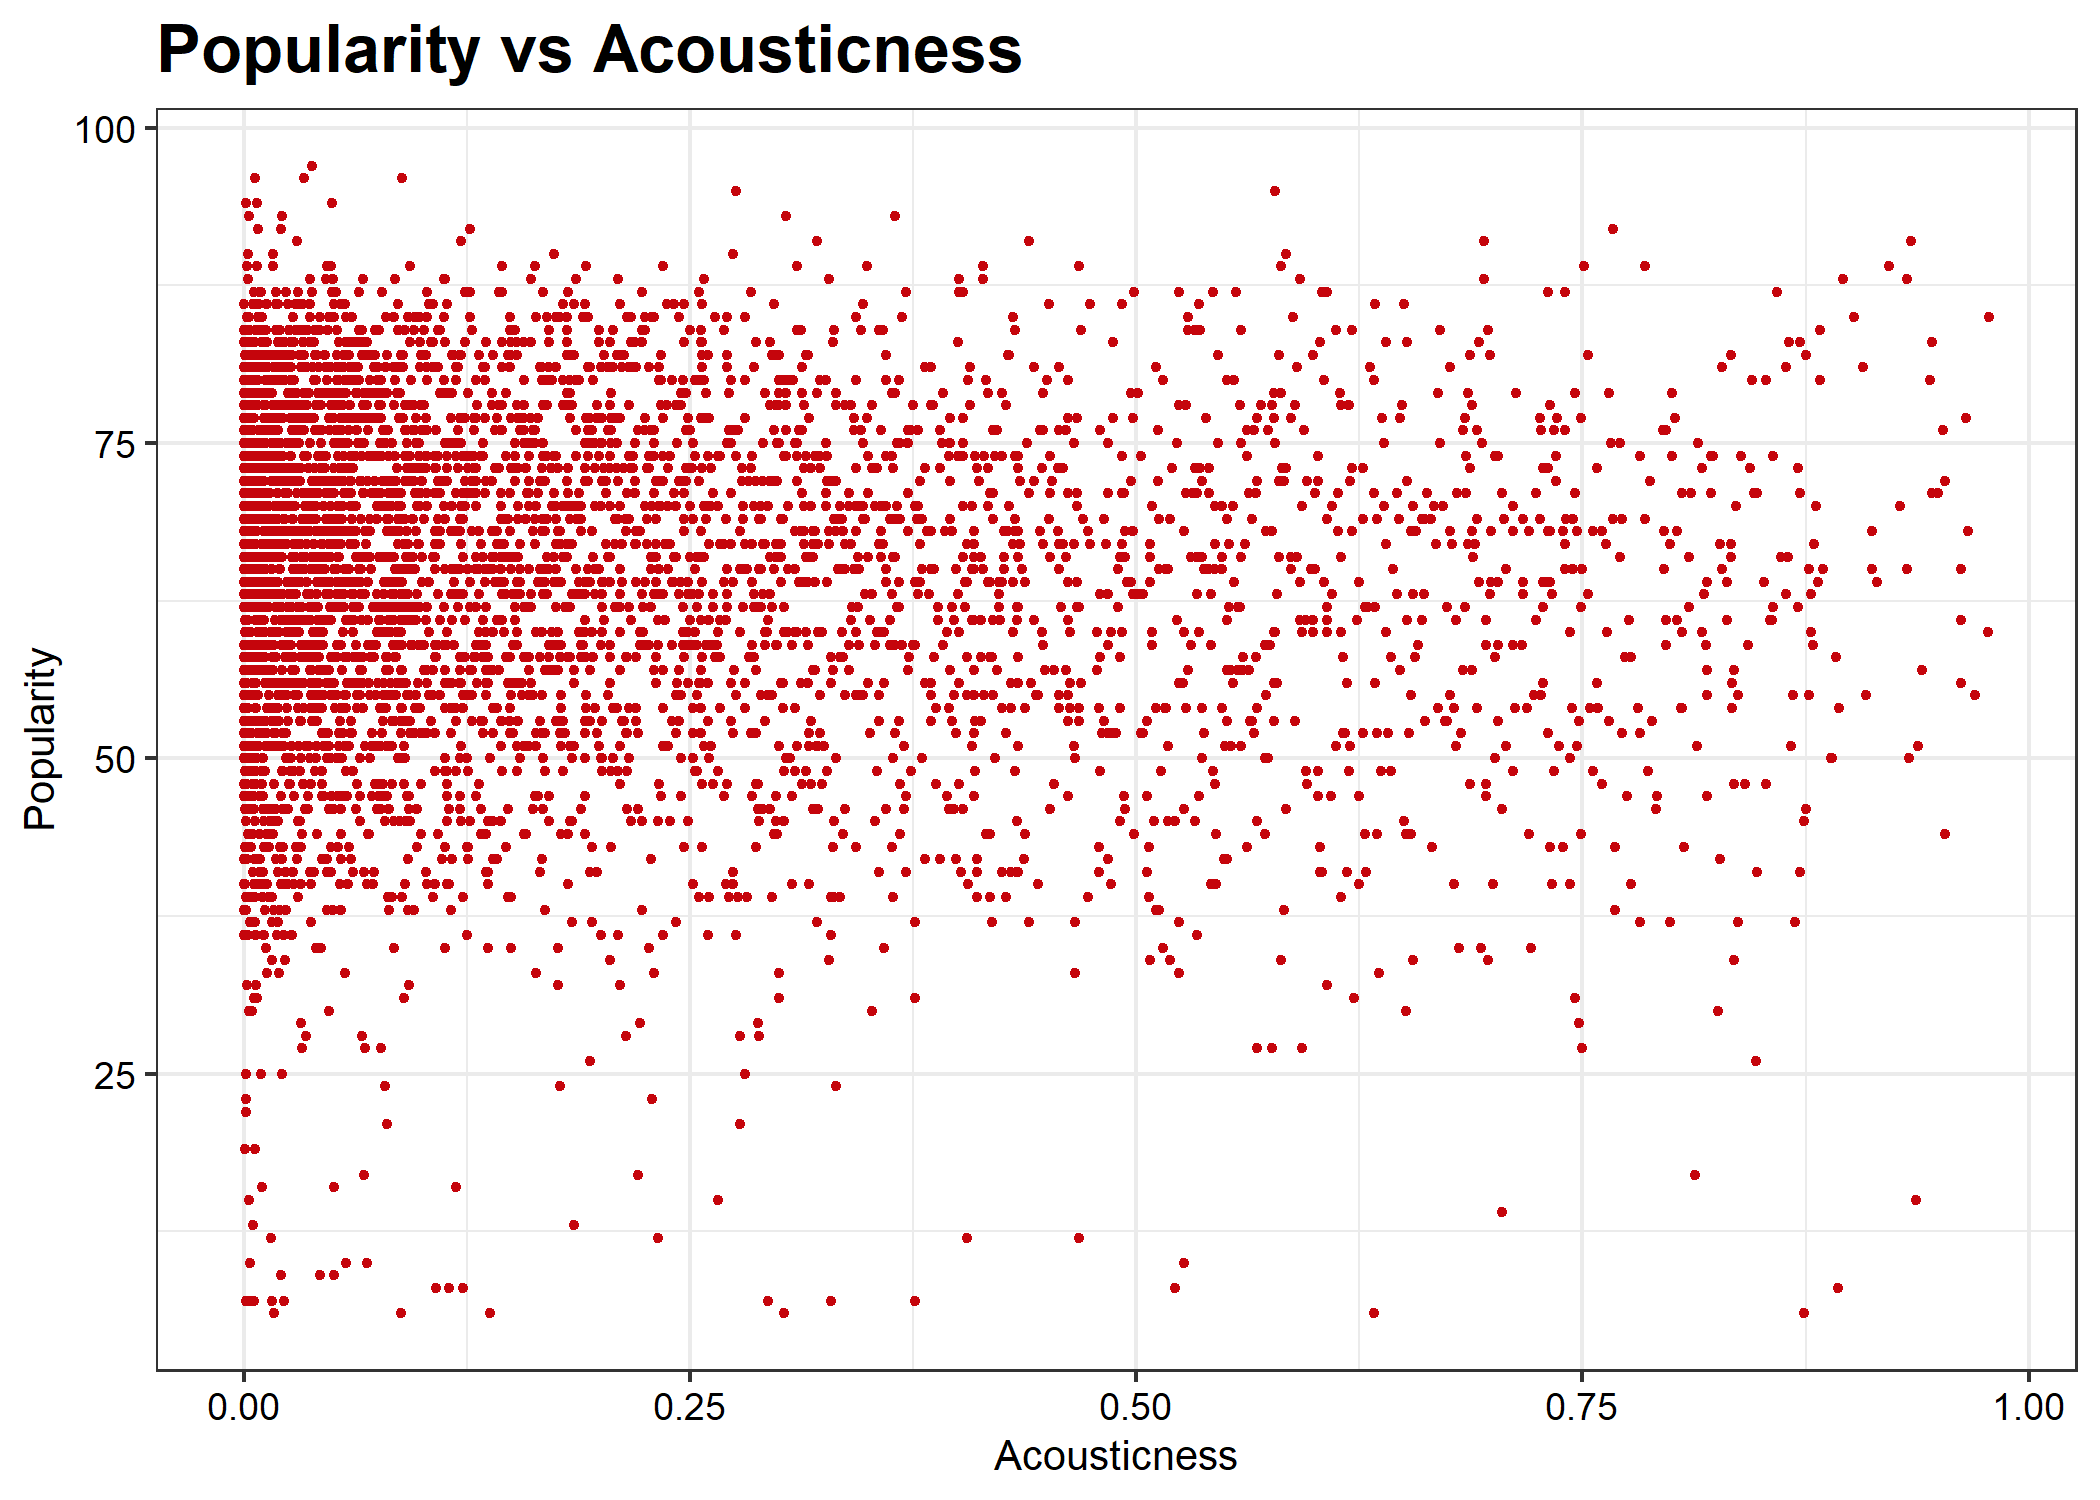
\includegraphics[width = \textwidth]{pop_vs_track_acousticness.png}
\caption{}
\label{fig:instrumentalness_trend}
\end{subfigure}
\begin{subfigure}[b]{0.5\textwidth}
\centering
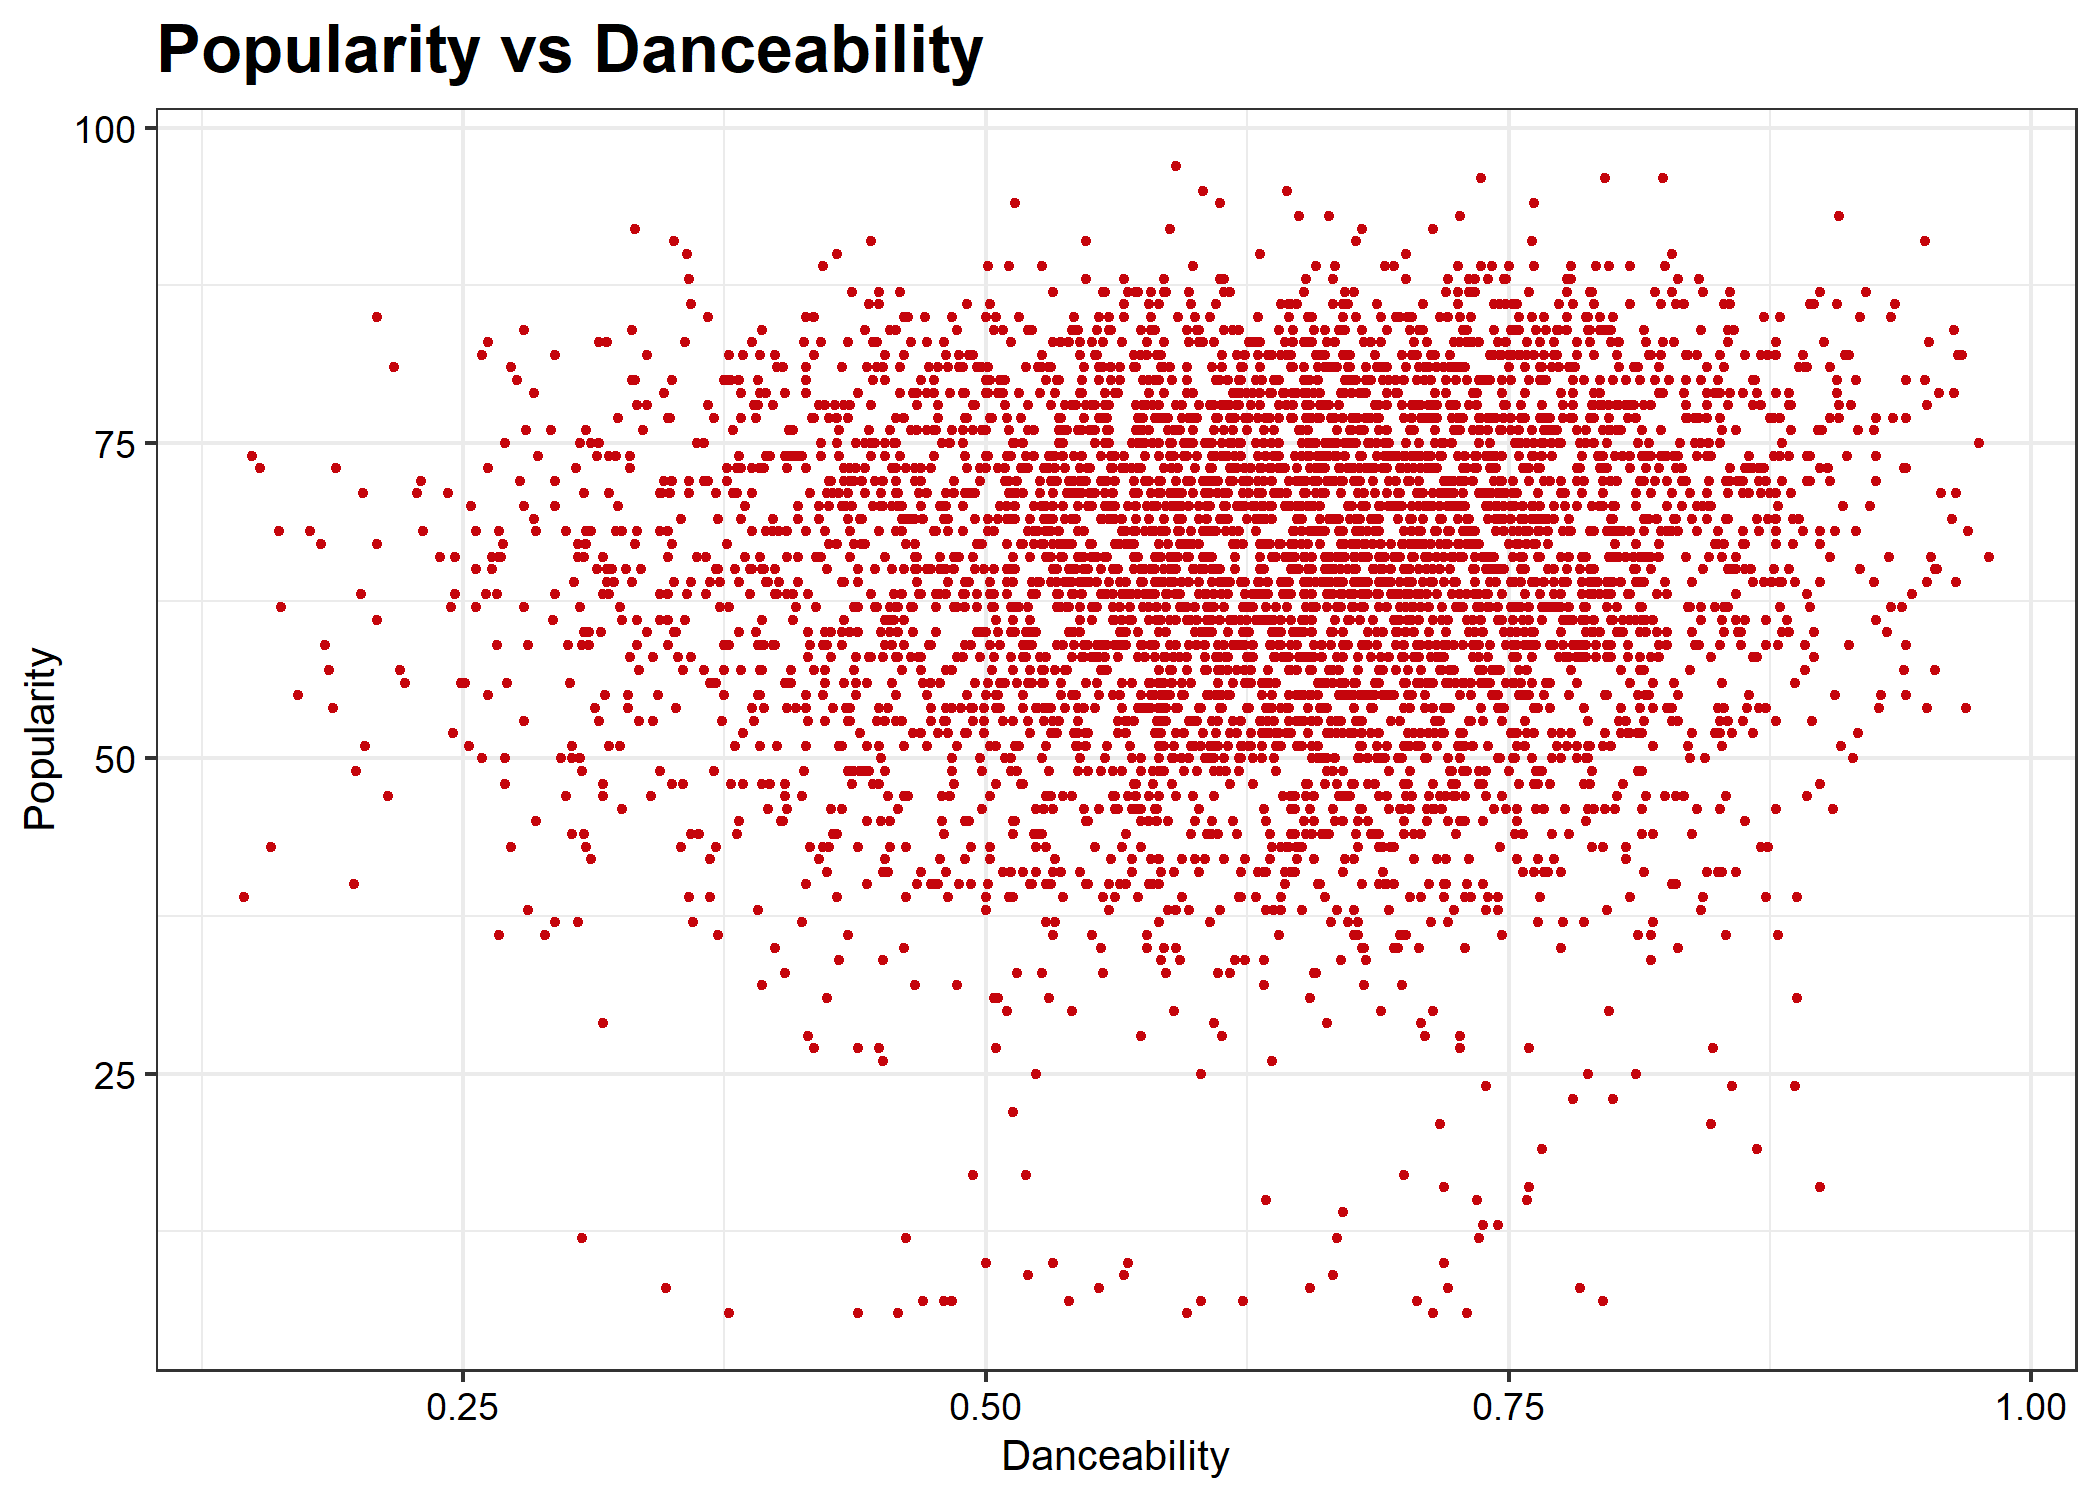
\includegraphics[width = \textwidth]{pop_vs_track_danceability.png}
\caption{}
\label{fig:loudness_trend}
\end{subfigure}
\begin{subfigure}[b]{0.5\textwidth}
\centering
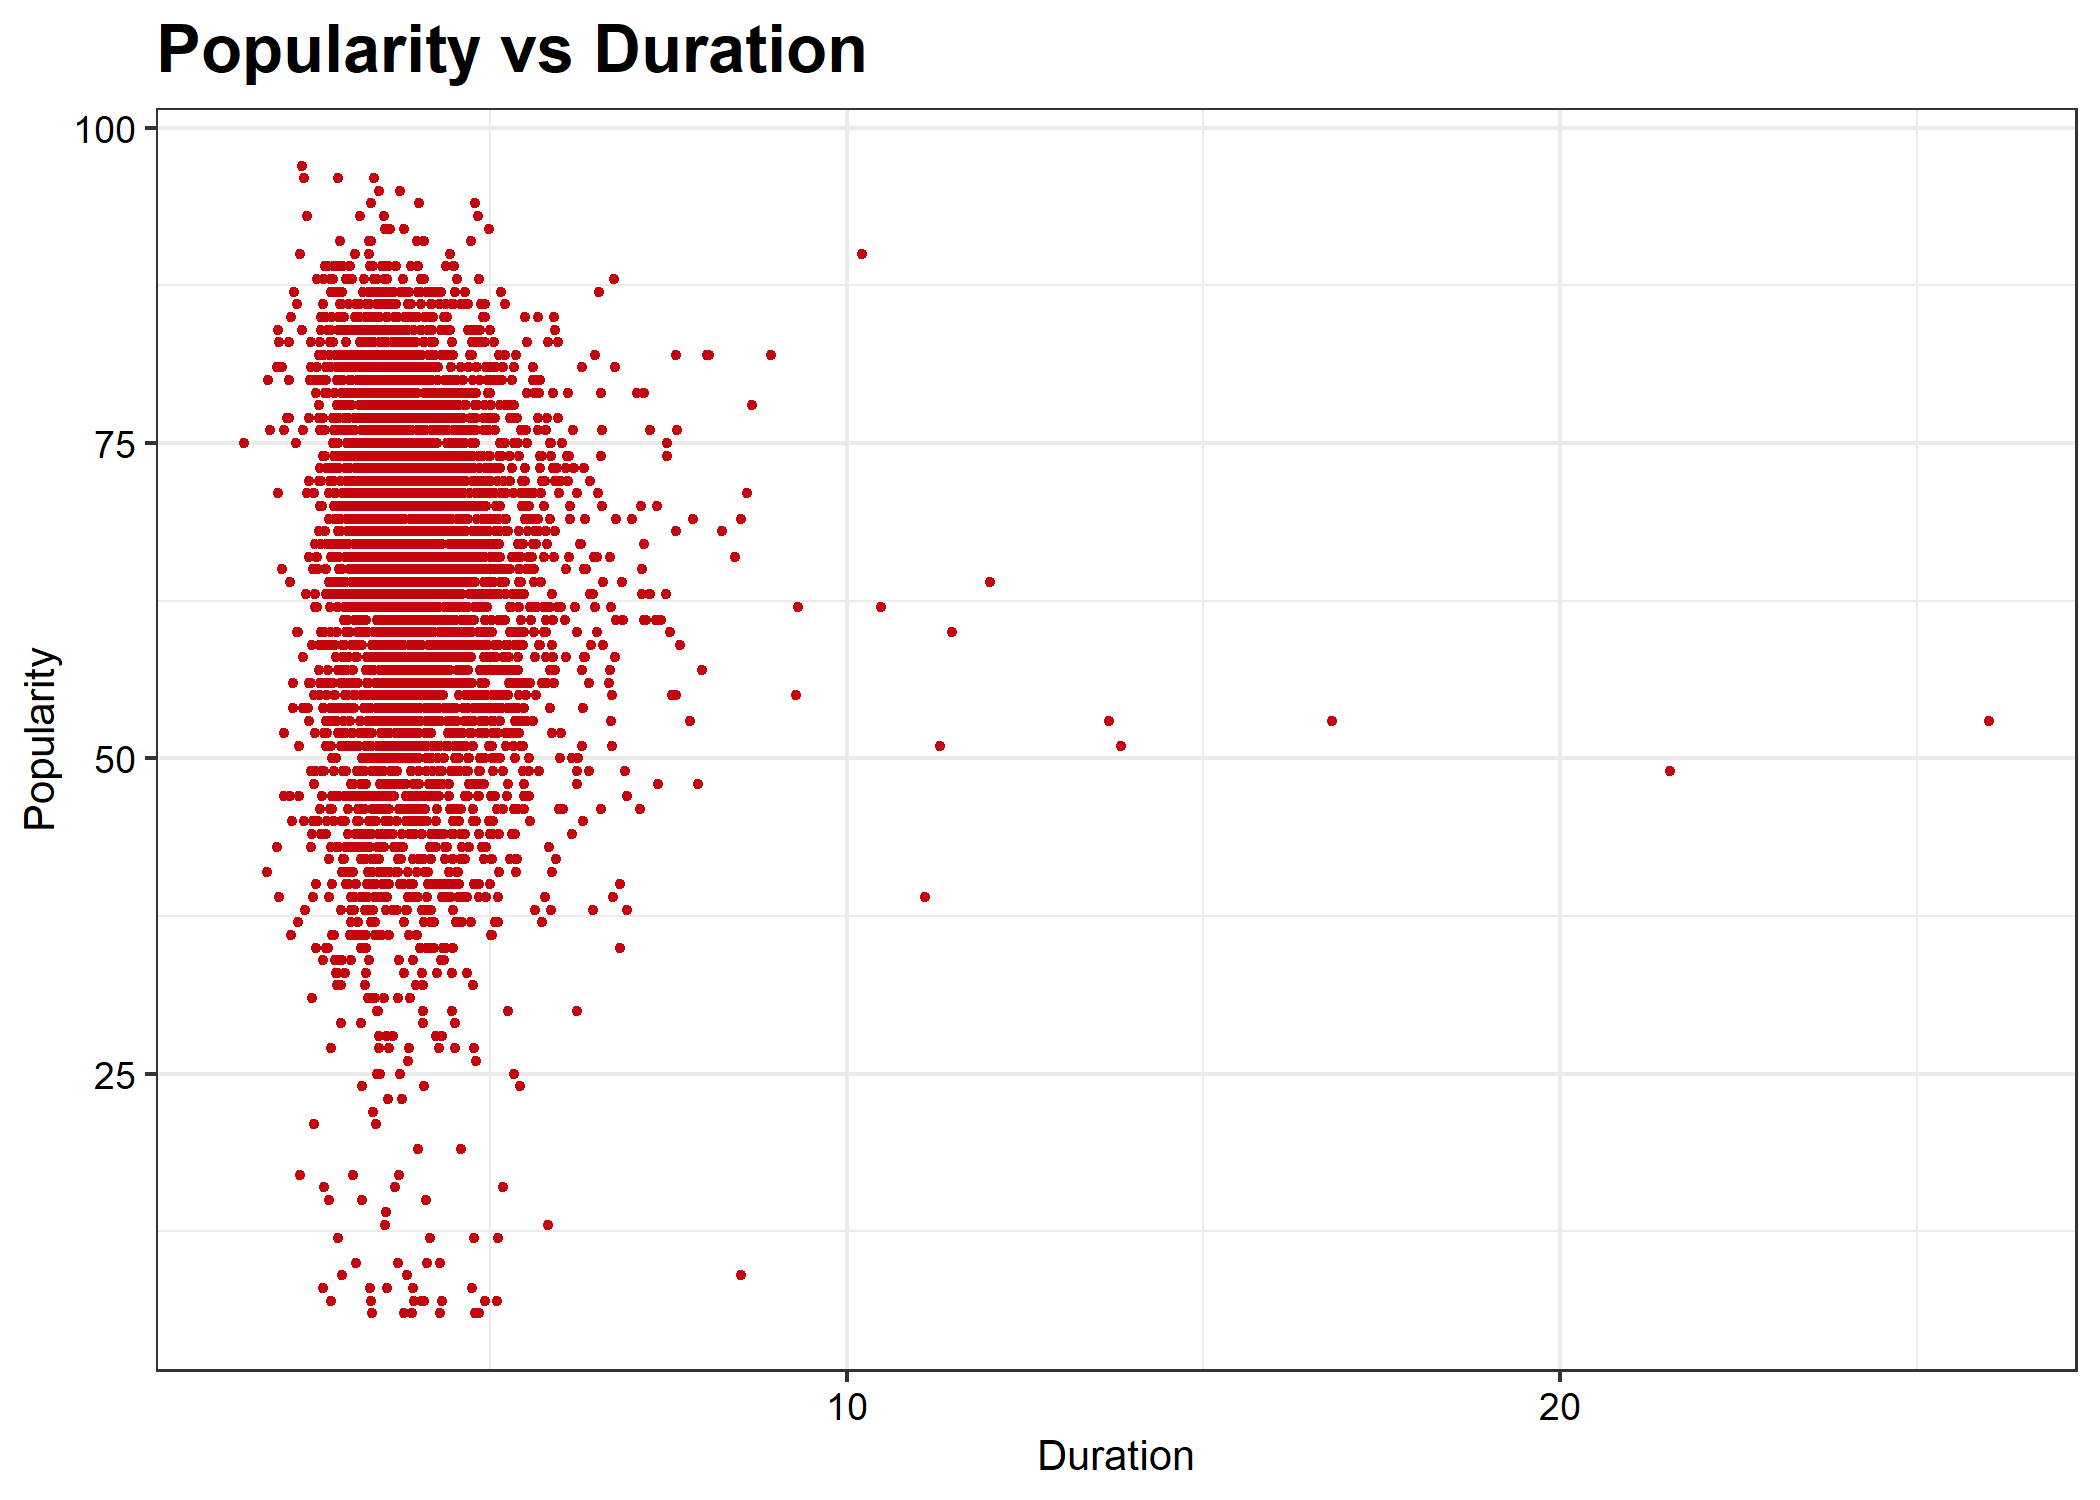
\includegraphics[width = \textwidth]{pop_vs_track_duration.png}
\caption{}
\label{fig:duration_trend}
\end{subfigure}
\end{figure}

\begin{figure}[H]
\ContinuedFloat
\begin{subfigure}[b]{0.5\textwidth}
\centering
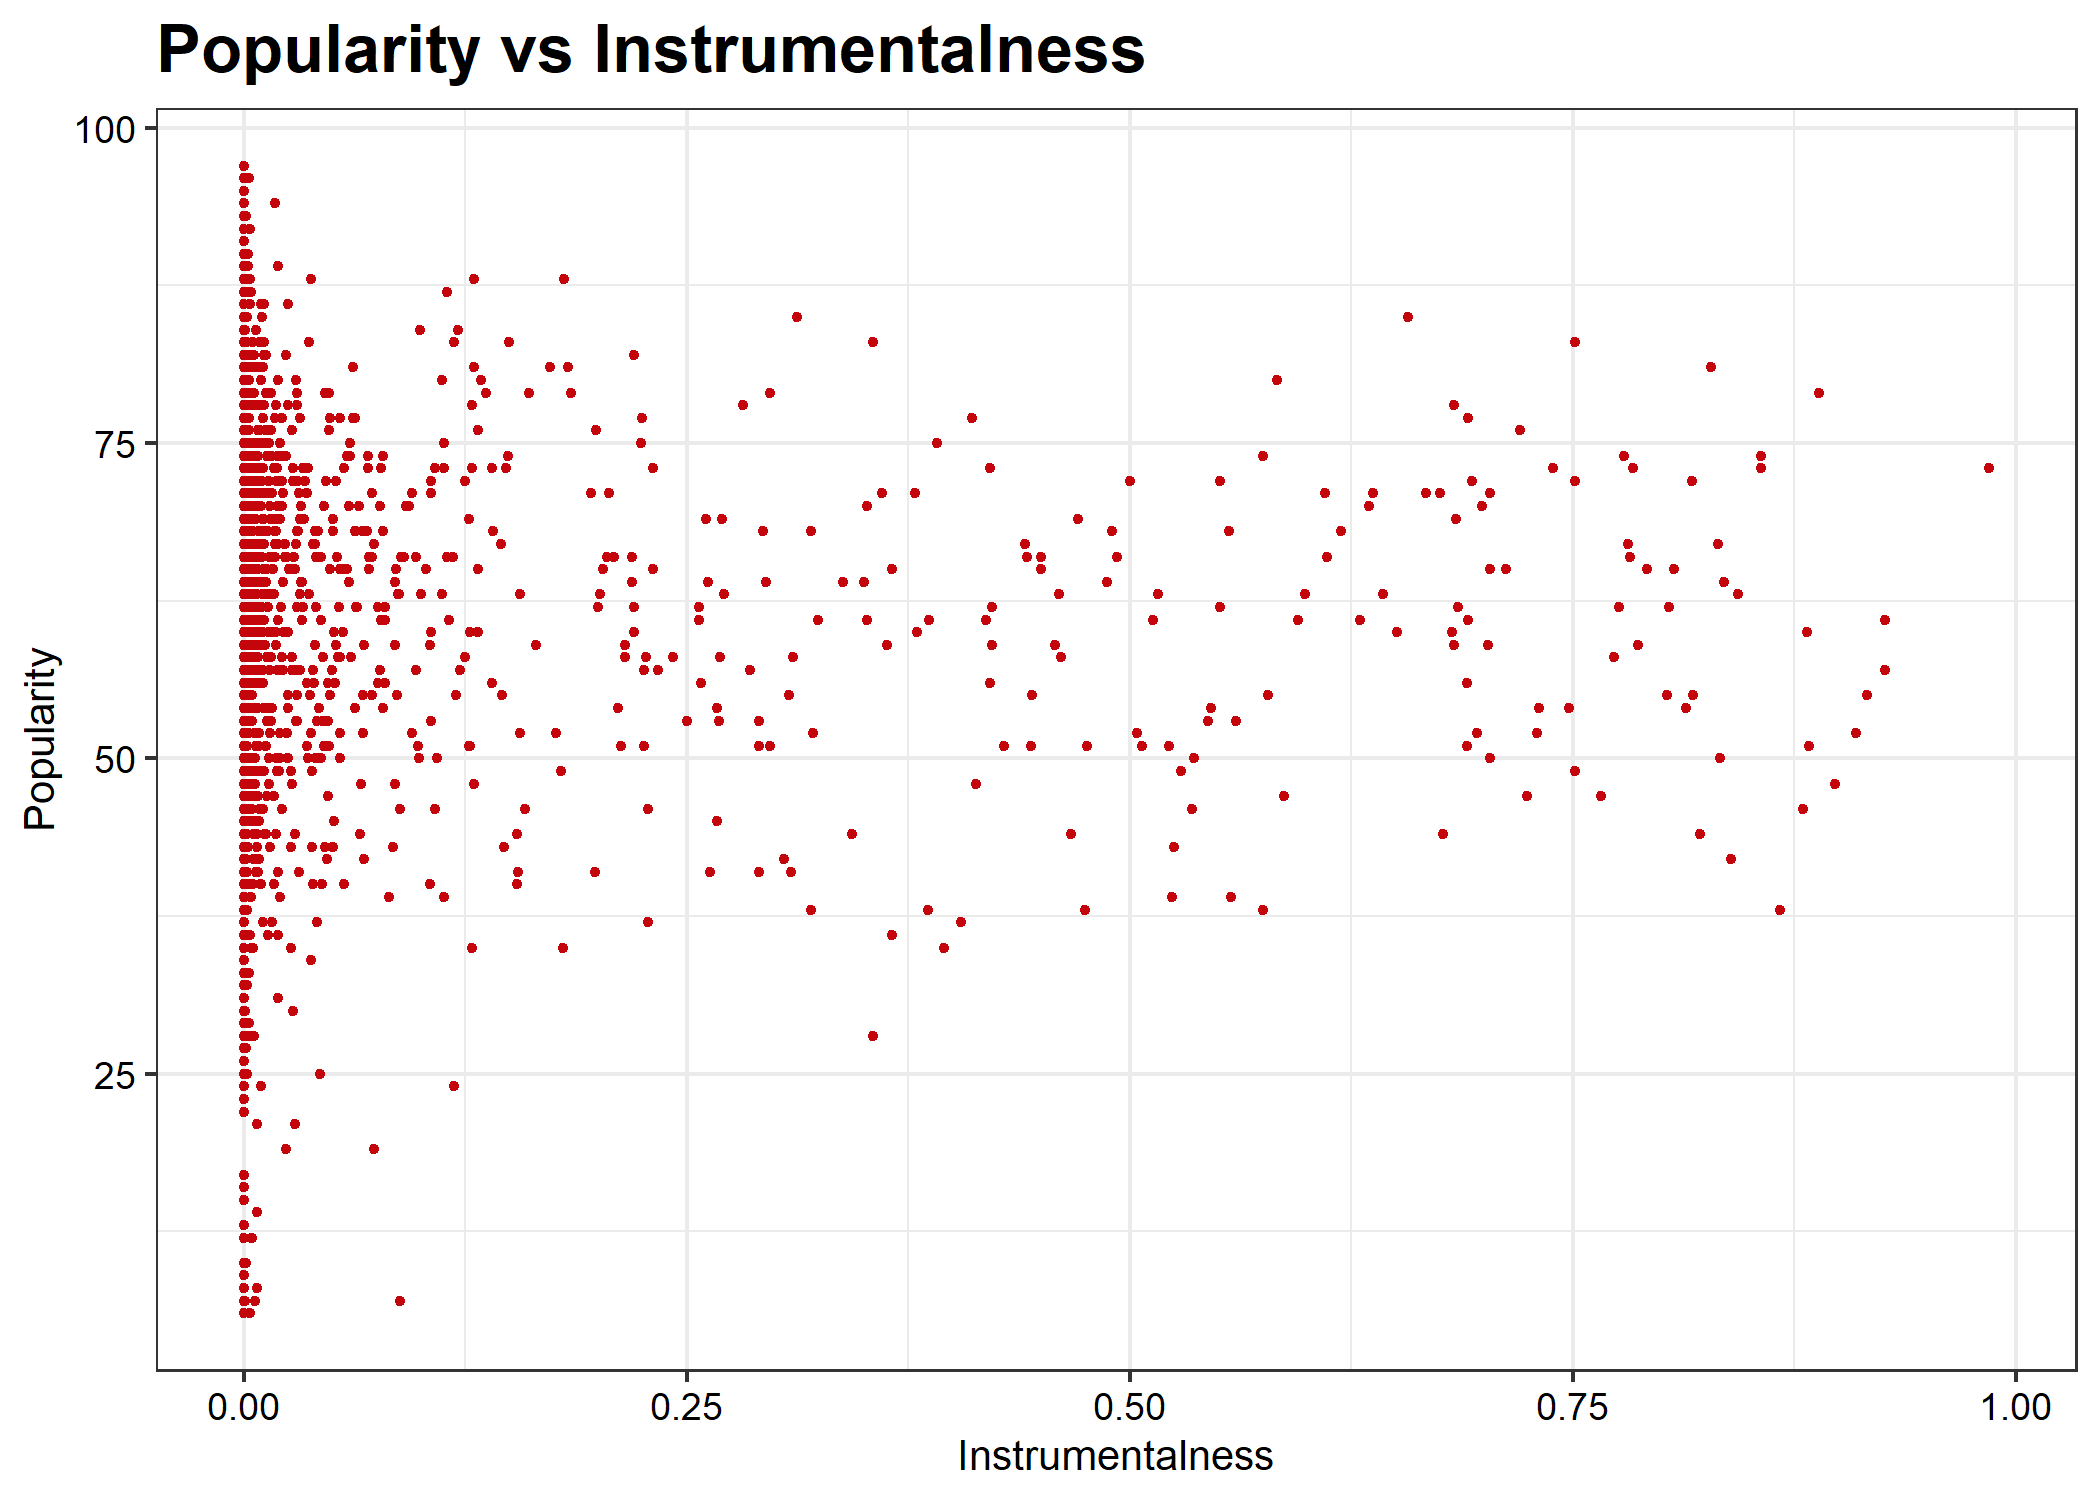
\includegraphics[width = \textwidth]{pop_vs_track_instrumentalness.png}
\caption{}
\label{fig:duration_trend}
\end{subfigure}
\begin{subfigure}[b]{0.5\textwidth}
\centering
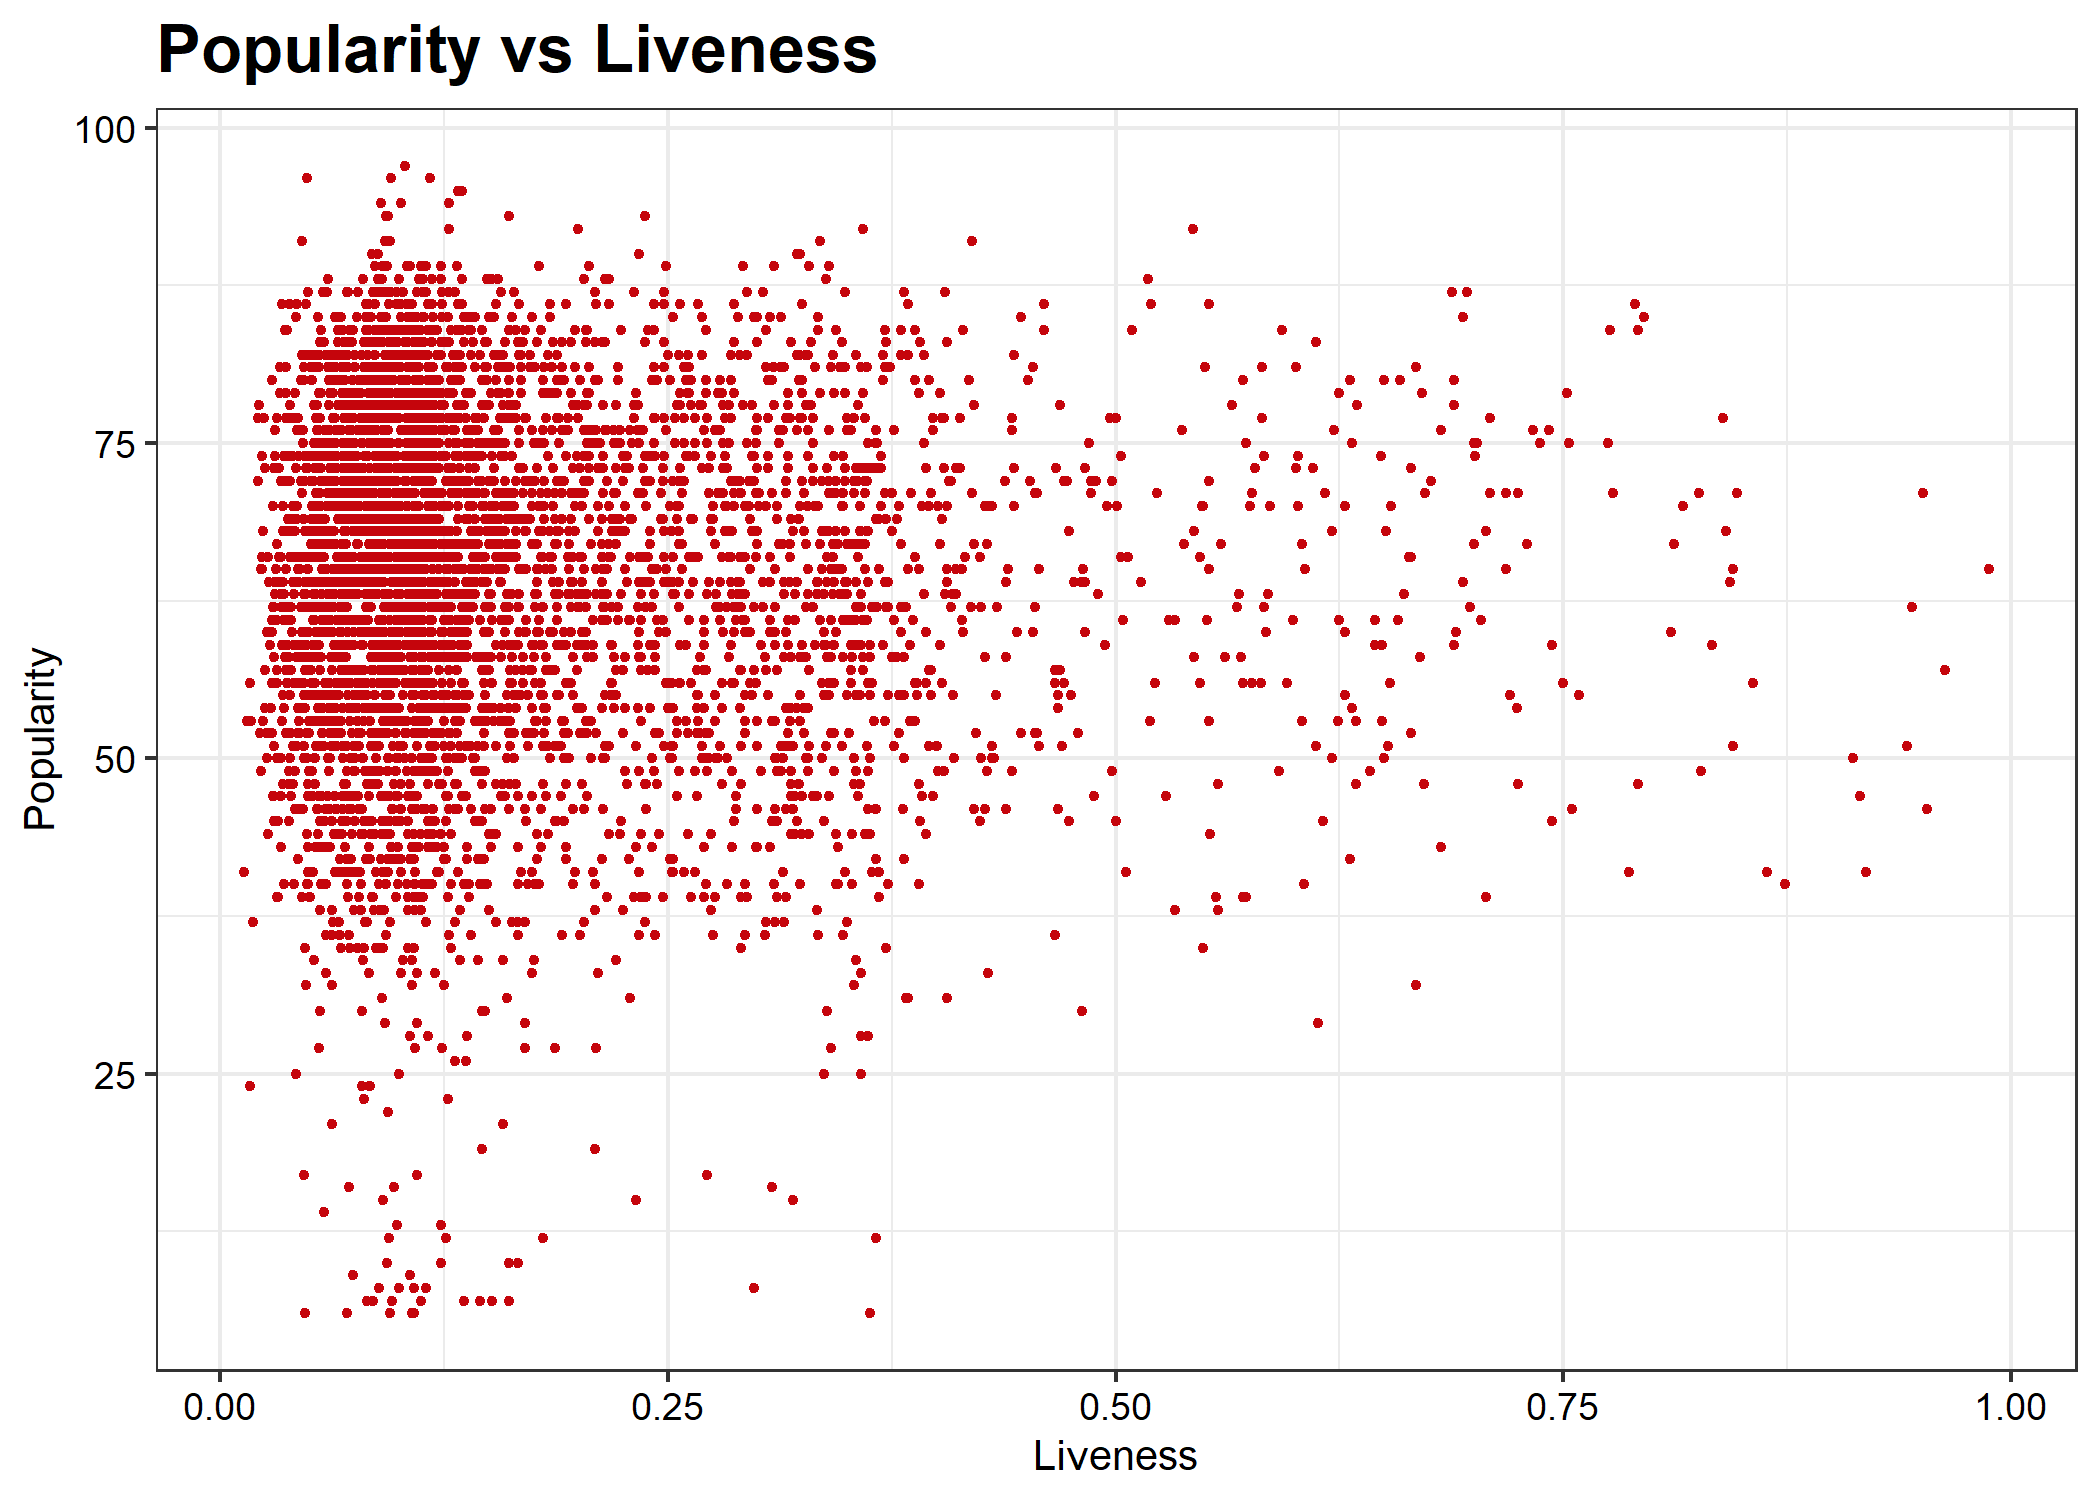
\includegraphics[width = \textwidth]{pop_vs_track_liveness.png}
\caption{}
\label{fig:duration_trend}
\end{subfigure}
\label{fig:multipart_figure}
\begin{subfigure}[b]{0.5\textwidth}
\centering
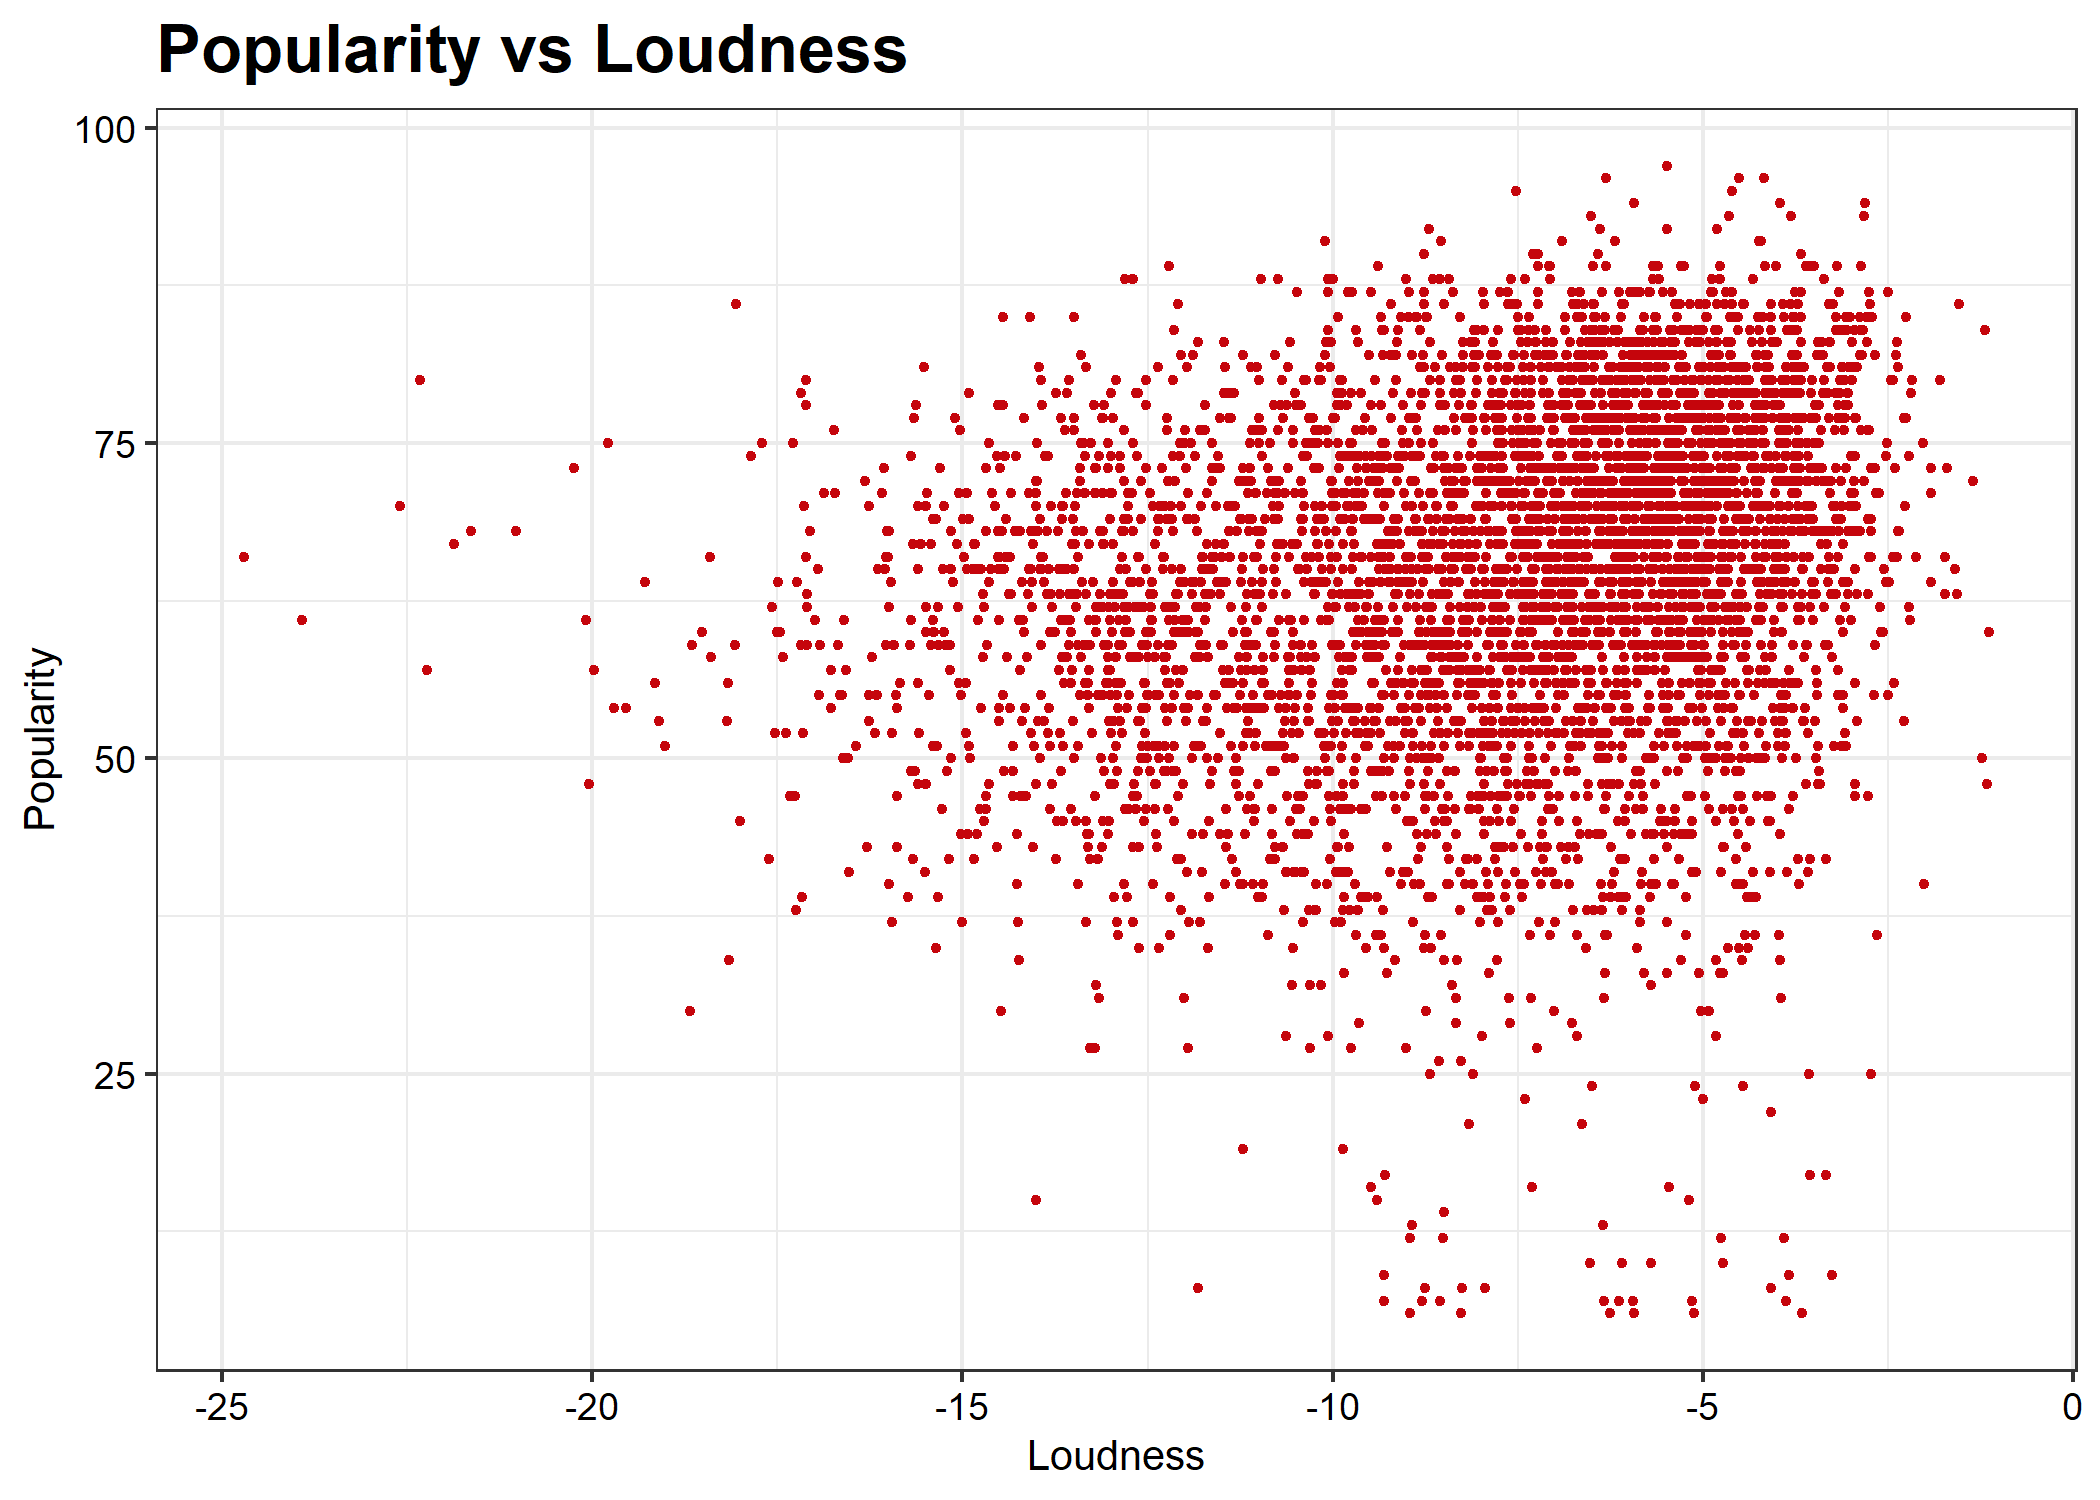
\includegraphics[width = \textwidth]{pop_vs_track_loudness.png}
\caption{}
\label{fig:duration_trend}
\end{subfigure}
\begin{subfigure}[b]{0.5\textwidth}
\centering
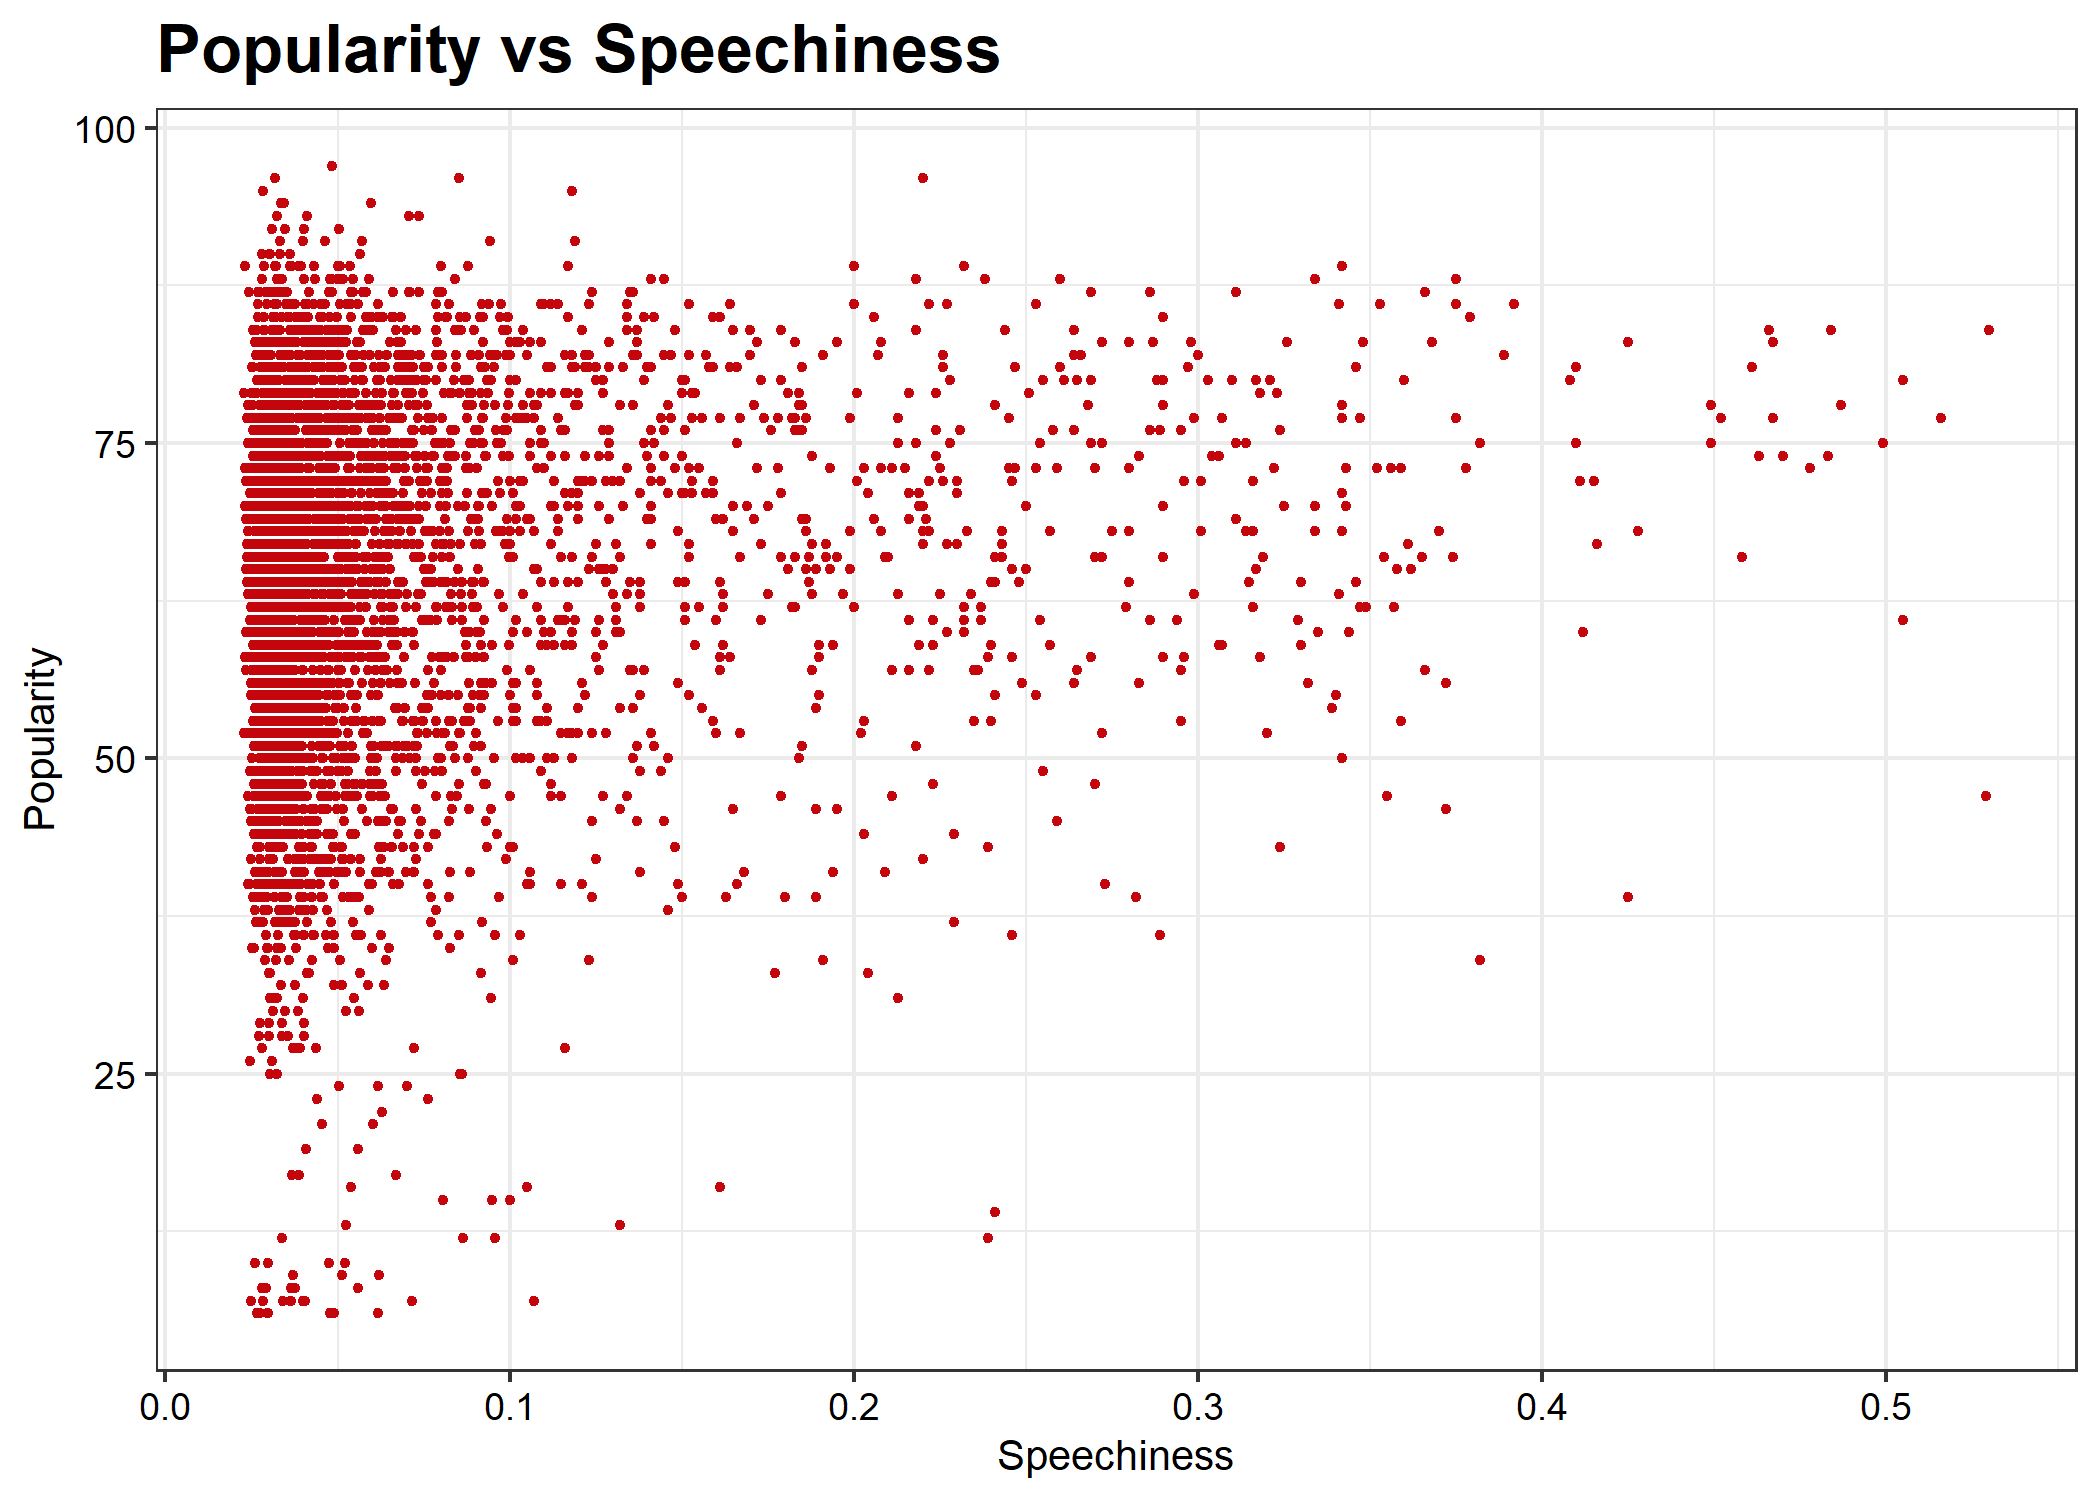
\includegraphics[width = \textwidth]{pop_vs_track_speechiness.png}
\caption{}
\label{fig:duration_trend}
\end{subfigure}
\begin{subfigure}[b]{0.5\textwidth}
\centering
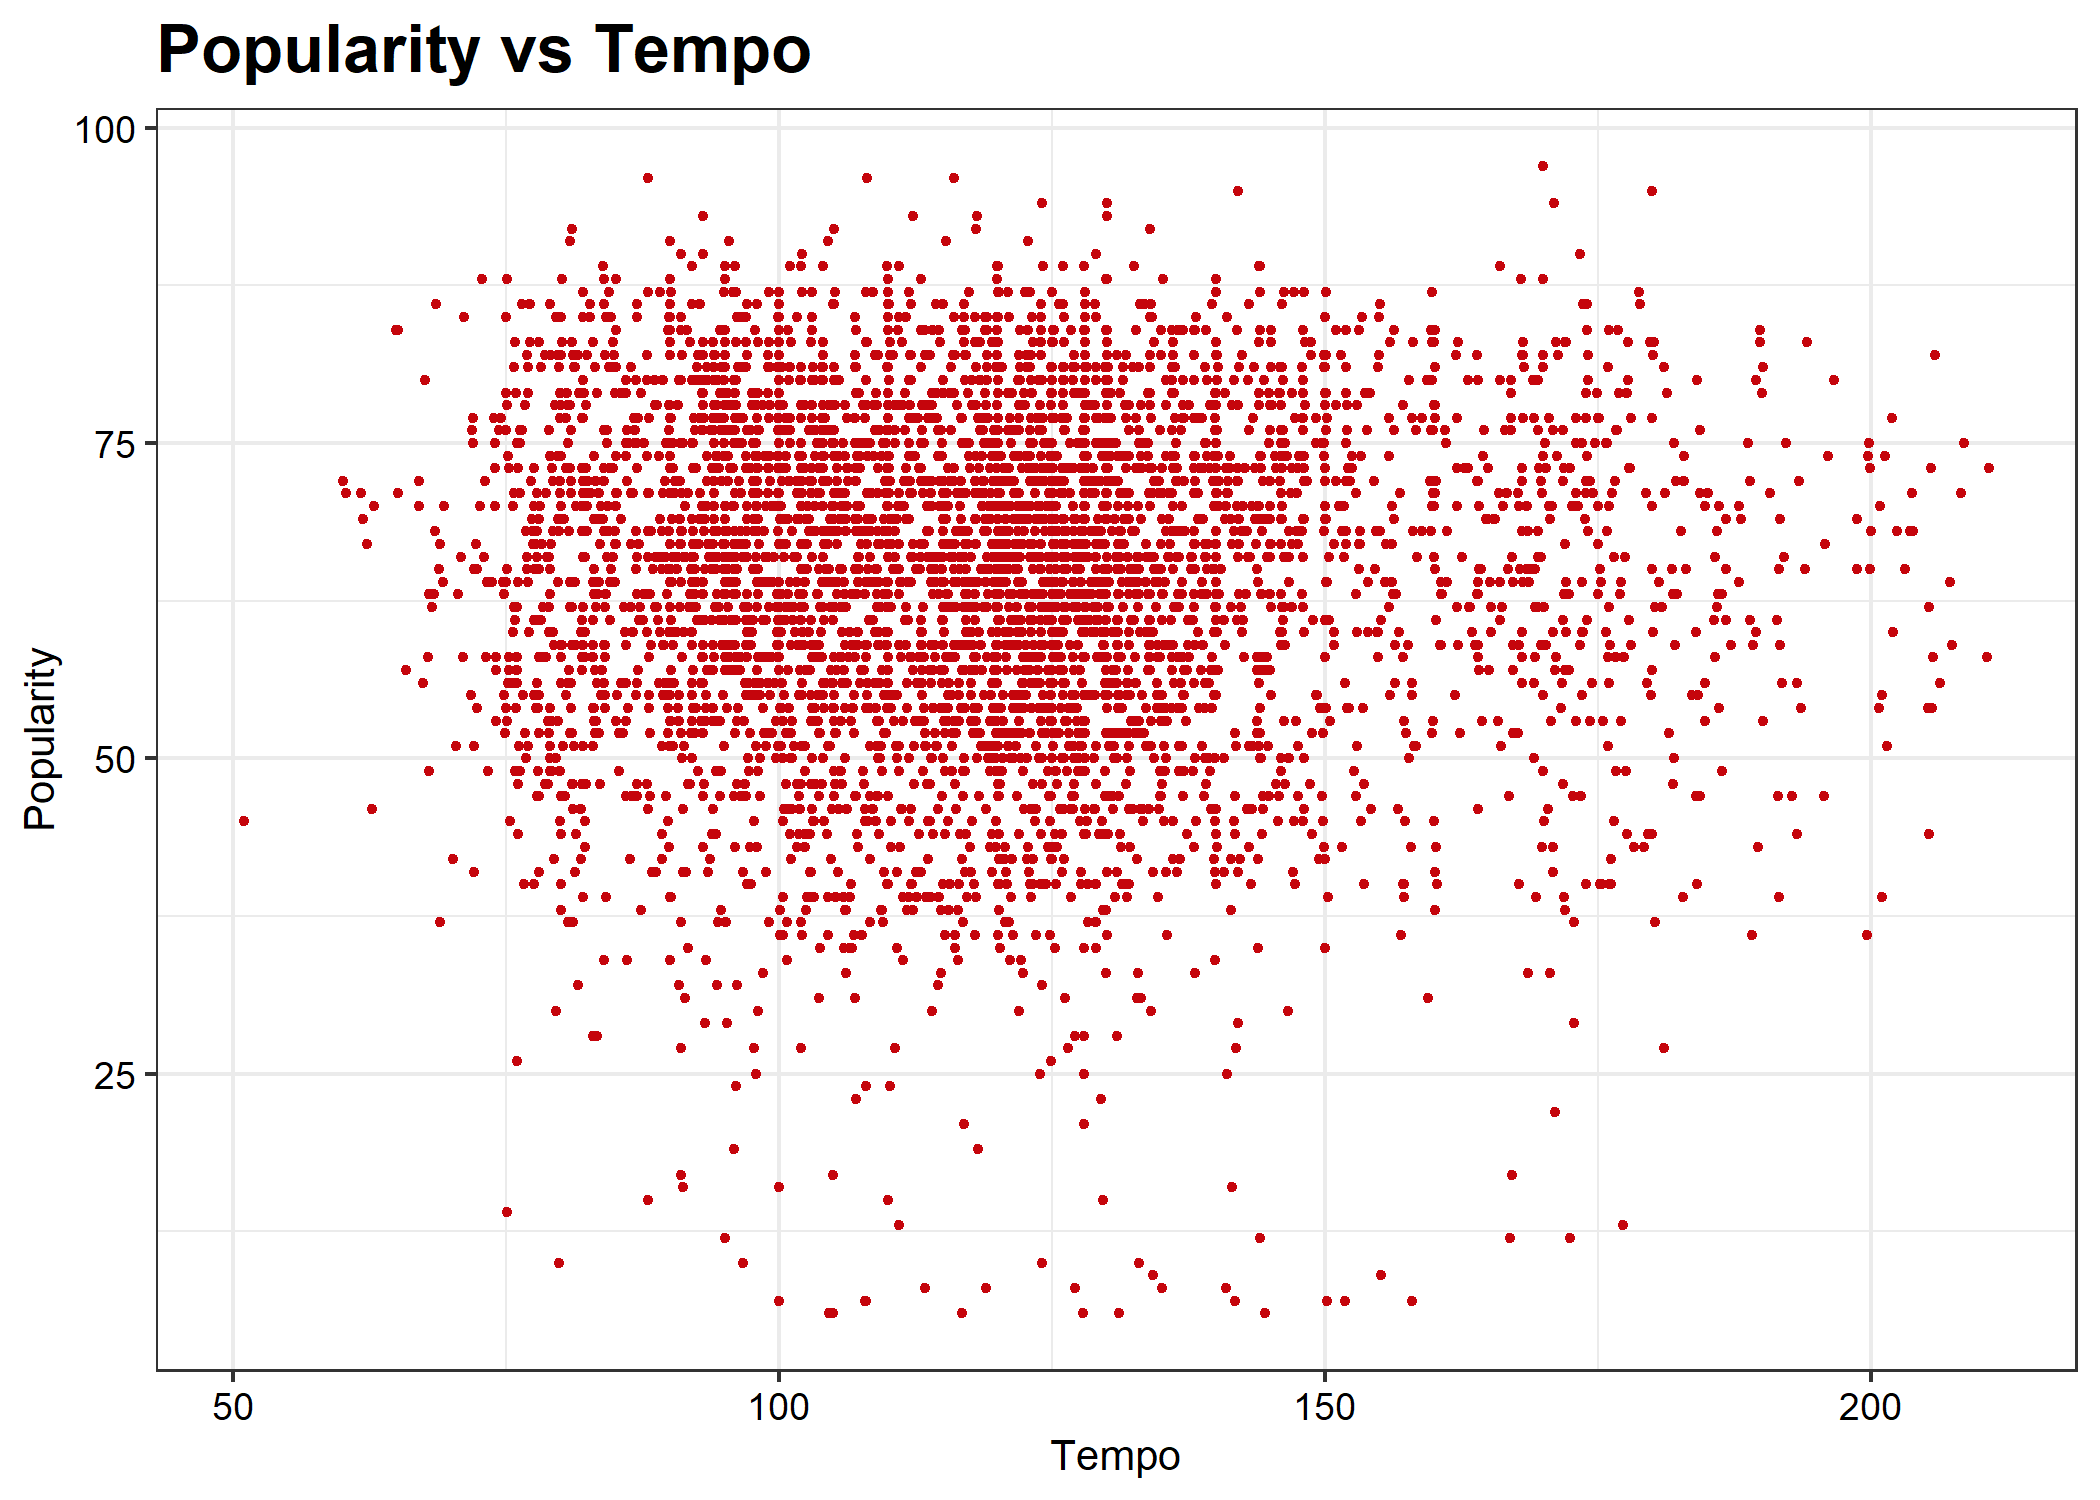
\includegraphics[width = \textwidth]{pop_vs_track_tempo.png}
\caption{}
\label{fig:duration_trend}
\end{subfigure}
\begin{subfigure}[b]{0.5\textwidth}
\centering
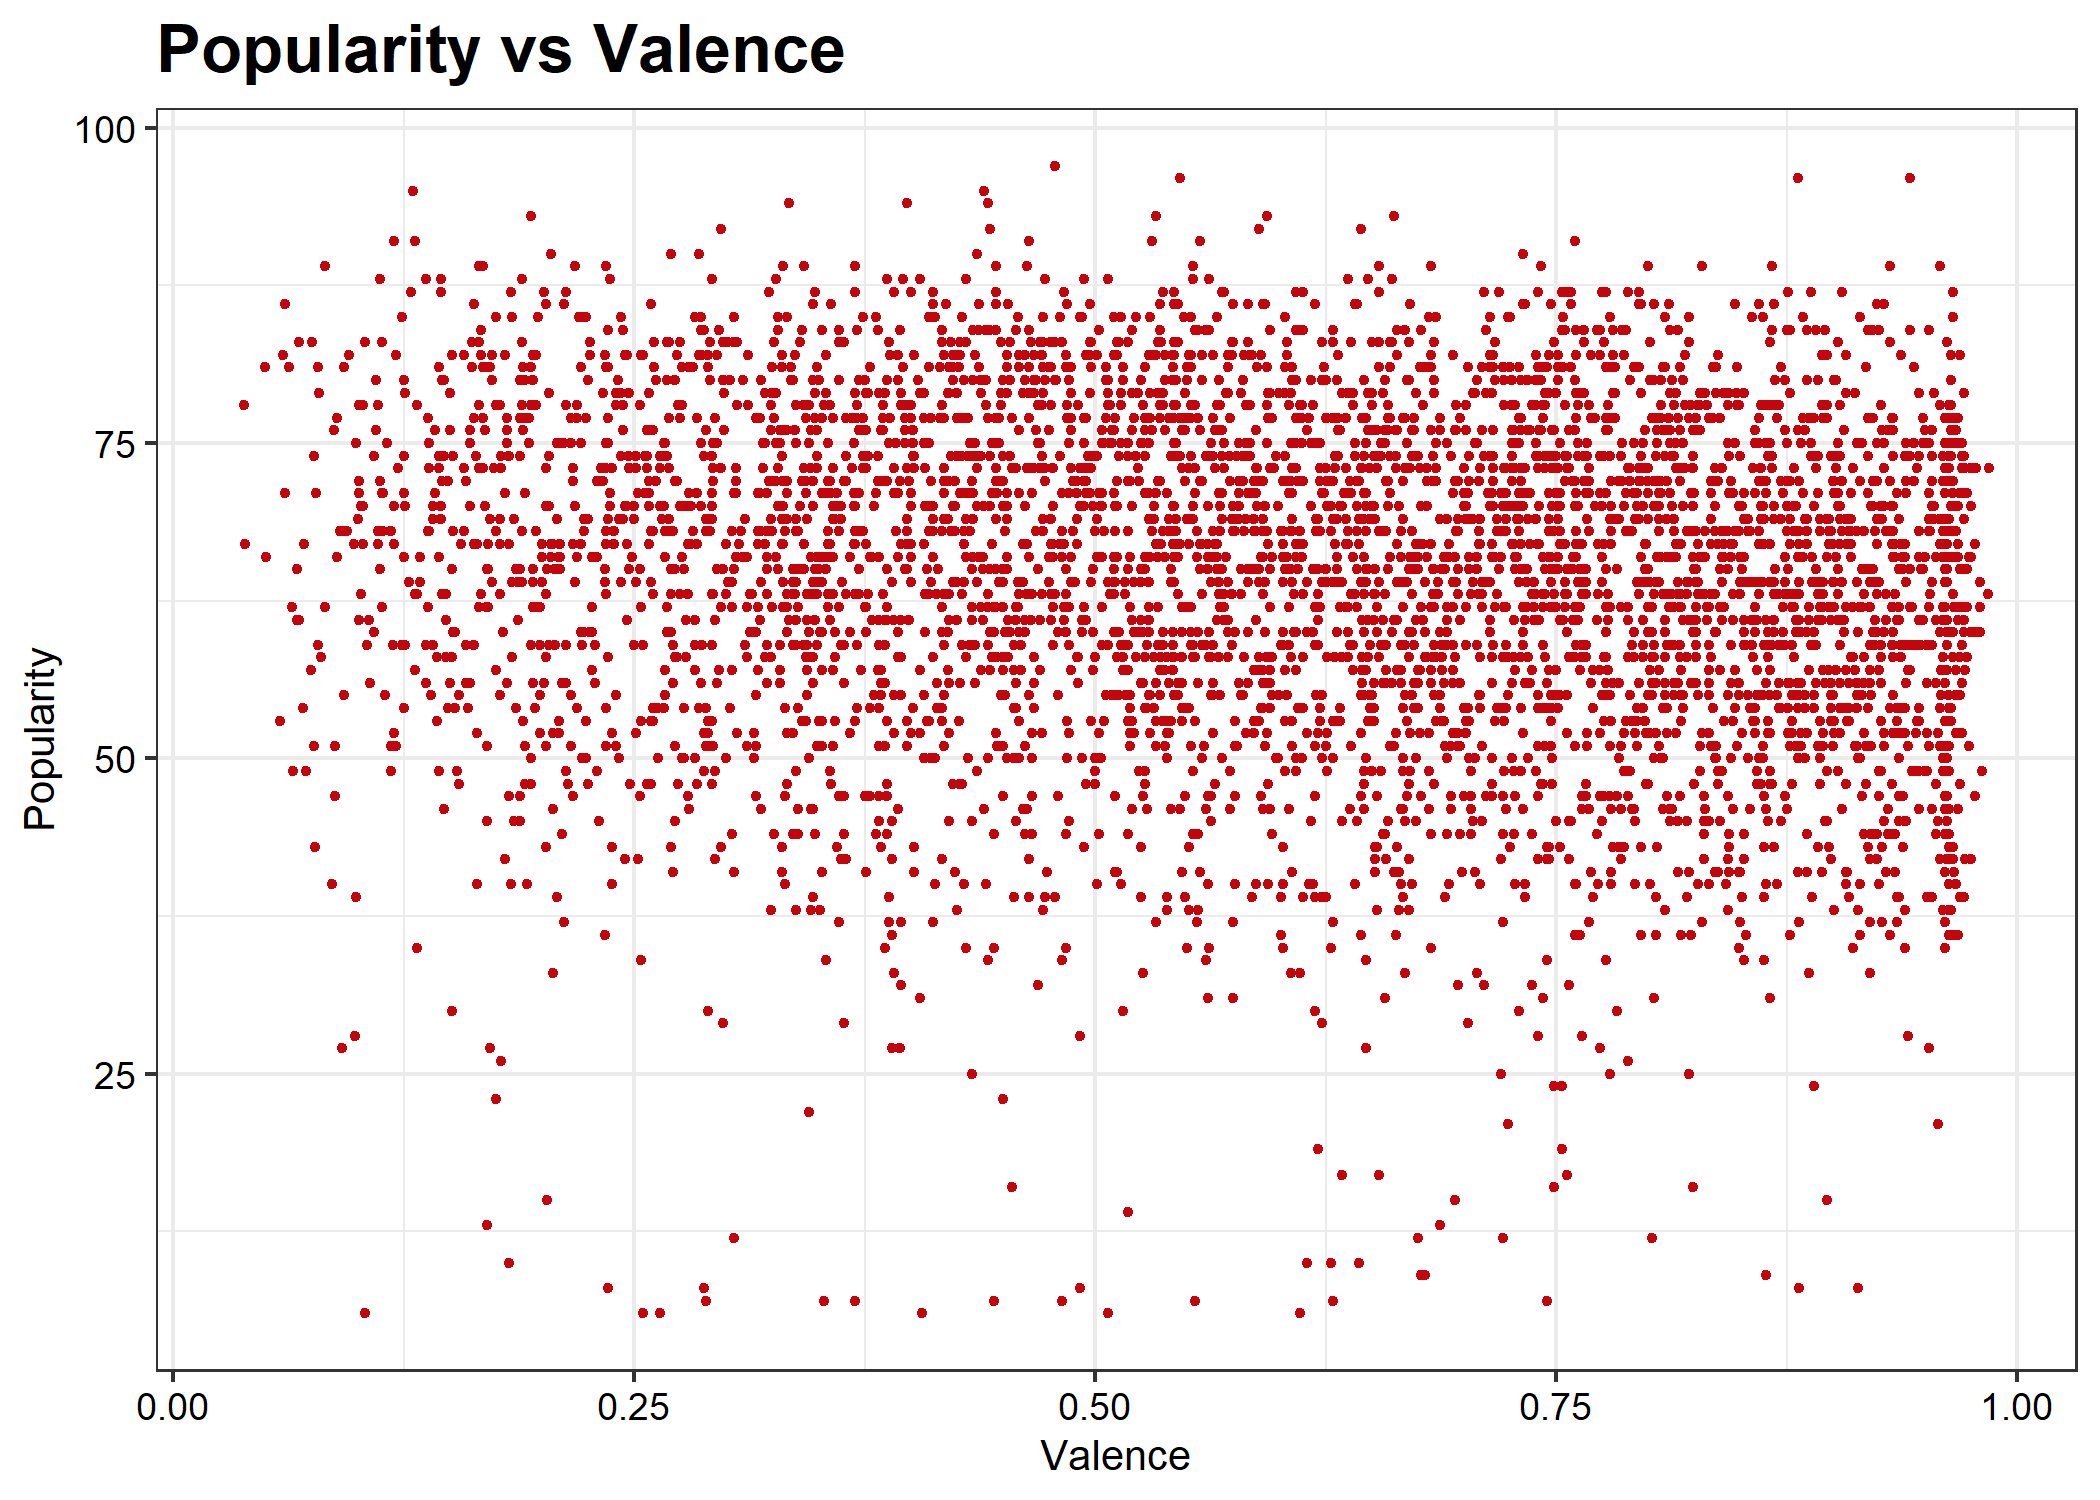
\includegraphics[width = \textwidth]{pop_vs_track_valence.png}
\caption{}
\label{fig:duration_trend}
\end{subfigure}
\caption{Response vs predictor scatter plots}
\end{figure}

Based on these figures, the task of predicting song popularity seems, at first glance, formidable. 

\section{Modeling}

I estimate a standard linear hierarchical model with $P=10$ predictors and $T=6$ decades by which the data are grouped. The model was fit using Stan. 

$\text{Let } Y_{it} \text{ denote the popularity of song } i \text{ in decade } t$. 

Then assume

\begin{align*}
Y_{it} \mid \alpha_t \ \bm{\beta}_{t} \ \sigma^2 & \sim N(\mu_{it}, \sigma^2) \text{ where } \mu_{it} = \alpha_t + x_i^T\bm{\beta}_{t} \\
\alpha_t \mid \mu_\alpha \ \tau_\alpha^2 & \sim N(\mu_{\alpha}, \tau^2_\alpha) \\
\beta_{jt} \mid \mu_{\beta_j} \ \tau_{\beta}^2 & \sim N(\mu_{\beta_j}, \tau_\beta^2) \\
\mu_\alpha & \sim N(50, 5) \\
\mu_{\beta_j} & \sim N(\Bar{\mu}_{\beta_{j}}, 1) \\
\tau_\beta^2 & \sim \text{Inv.Gamma}(1.5, 1) \\
\tau_\alpha^2 & \sim \text{Inv.Gamma}(1.5, 1) \\
\sigma^2 & \sim \text{Inv.Gamma}(1.5, 0.3)
\end{align*}

The hierarchical structure defined above allows for posterior intercepts and slopes to vary by decade. This is important since each decade has a variable base-level popularity, and we assume the effect of each predictor on popularity may vary by decade. $\bm{\beta}_{t}$ is the length-$P$ vector of predictor coefficients for decade $t$. Within the second layer, $\beta_{jt}$ is therefor the $j$-th coefficient in decade $t$ and $\alpha_t$ is the intercept within decade $t$. The third layer defines priors and their hyperparameters, which were set using a combination of prior predictive checks and a priori beliefs. In particular, the hyperparameters $\Bar{\mu}_{\beta_{j}}$ were set to reflect a priori beliefs regarding the sign of each coefficient. It was set to $-0.10$ for instrumentalness, acousticness, liveness, and duration, reflecting the belief that the posterior mean for the coefficients associated with these predictors should be negative. For all other predictors, it was set to $0.10$ (since, for instance, we expect the relationship between popularity and danceability to be positive). The relatively small absolute value of $0.10$ was chosen so as to not be overly strong. Further, note that the $\beta_{jt}$ coefficients share a variance parameter. That is, the variability of the effect of one predictor is assumed to be the same as the variability of the effect of some other predictor. 

Some numerical summaries are provided below:

\begin{table}[H]
\centering
\caption{Numerical Summary Statistics}
\label{tab:results}
\def\arraystretch{1.5}
\begin{tabular}{l  p{2cm}  p{3cm}} % note the 
\hline
Quantity & Value \\ \hline
RMSE & 11.59 \\
MAPE & 19.83\% \\
$R^2$ & 0.295 \\
$\sigma^2$ & 11.62 \\
Mean ESS & 3918 \\
Mean $\hat{R}$ & 1.00003
\label{table:model_sum}
\end{tabular}
\end{table}

The model is clearly not predicting particularly well; on average, predictions miss by about 20\% (though much of this is due to the model's difficulty when predicting low popularity songs---for songs with observed popularity greater than 0.30, the RMSE falls to 9.85 and the MAPE falls to 13.3\%). It does, at least, explain approximately 30\% of variability. Convergence diagnostics (ESS and $\hat{R}$) were acceptable for all parameters. 

To get a better idea of the model's performance, we can see how the posterior predictive distribution updated the prior predictive distribution.

\begin{figure}[H]
\begin{subfigure}[b]{0.5\textwidth}
\centering
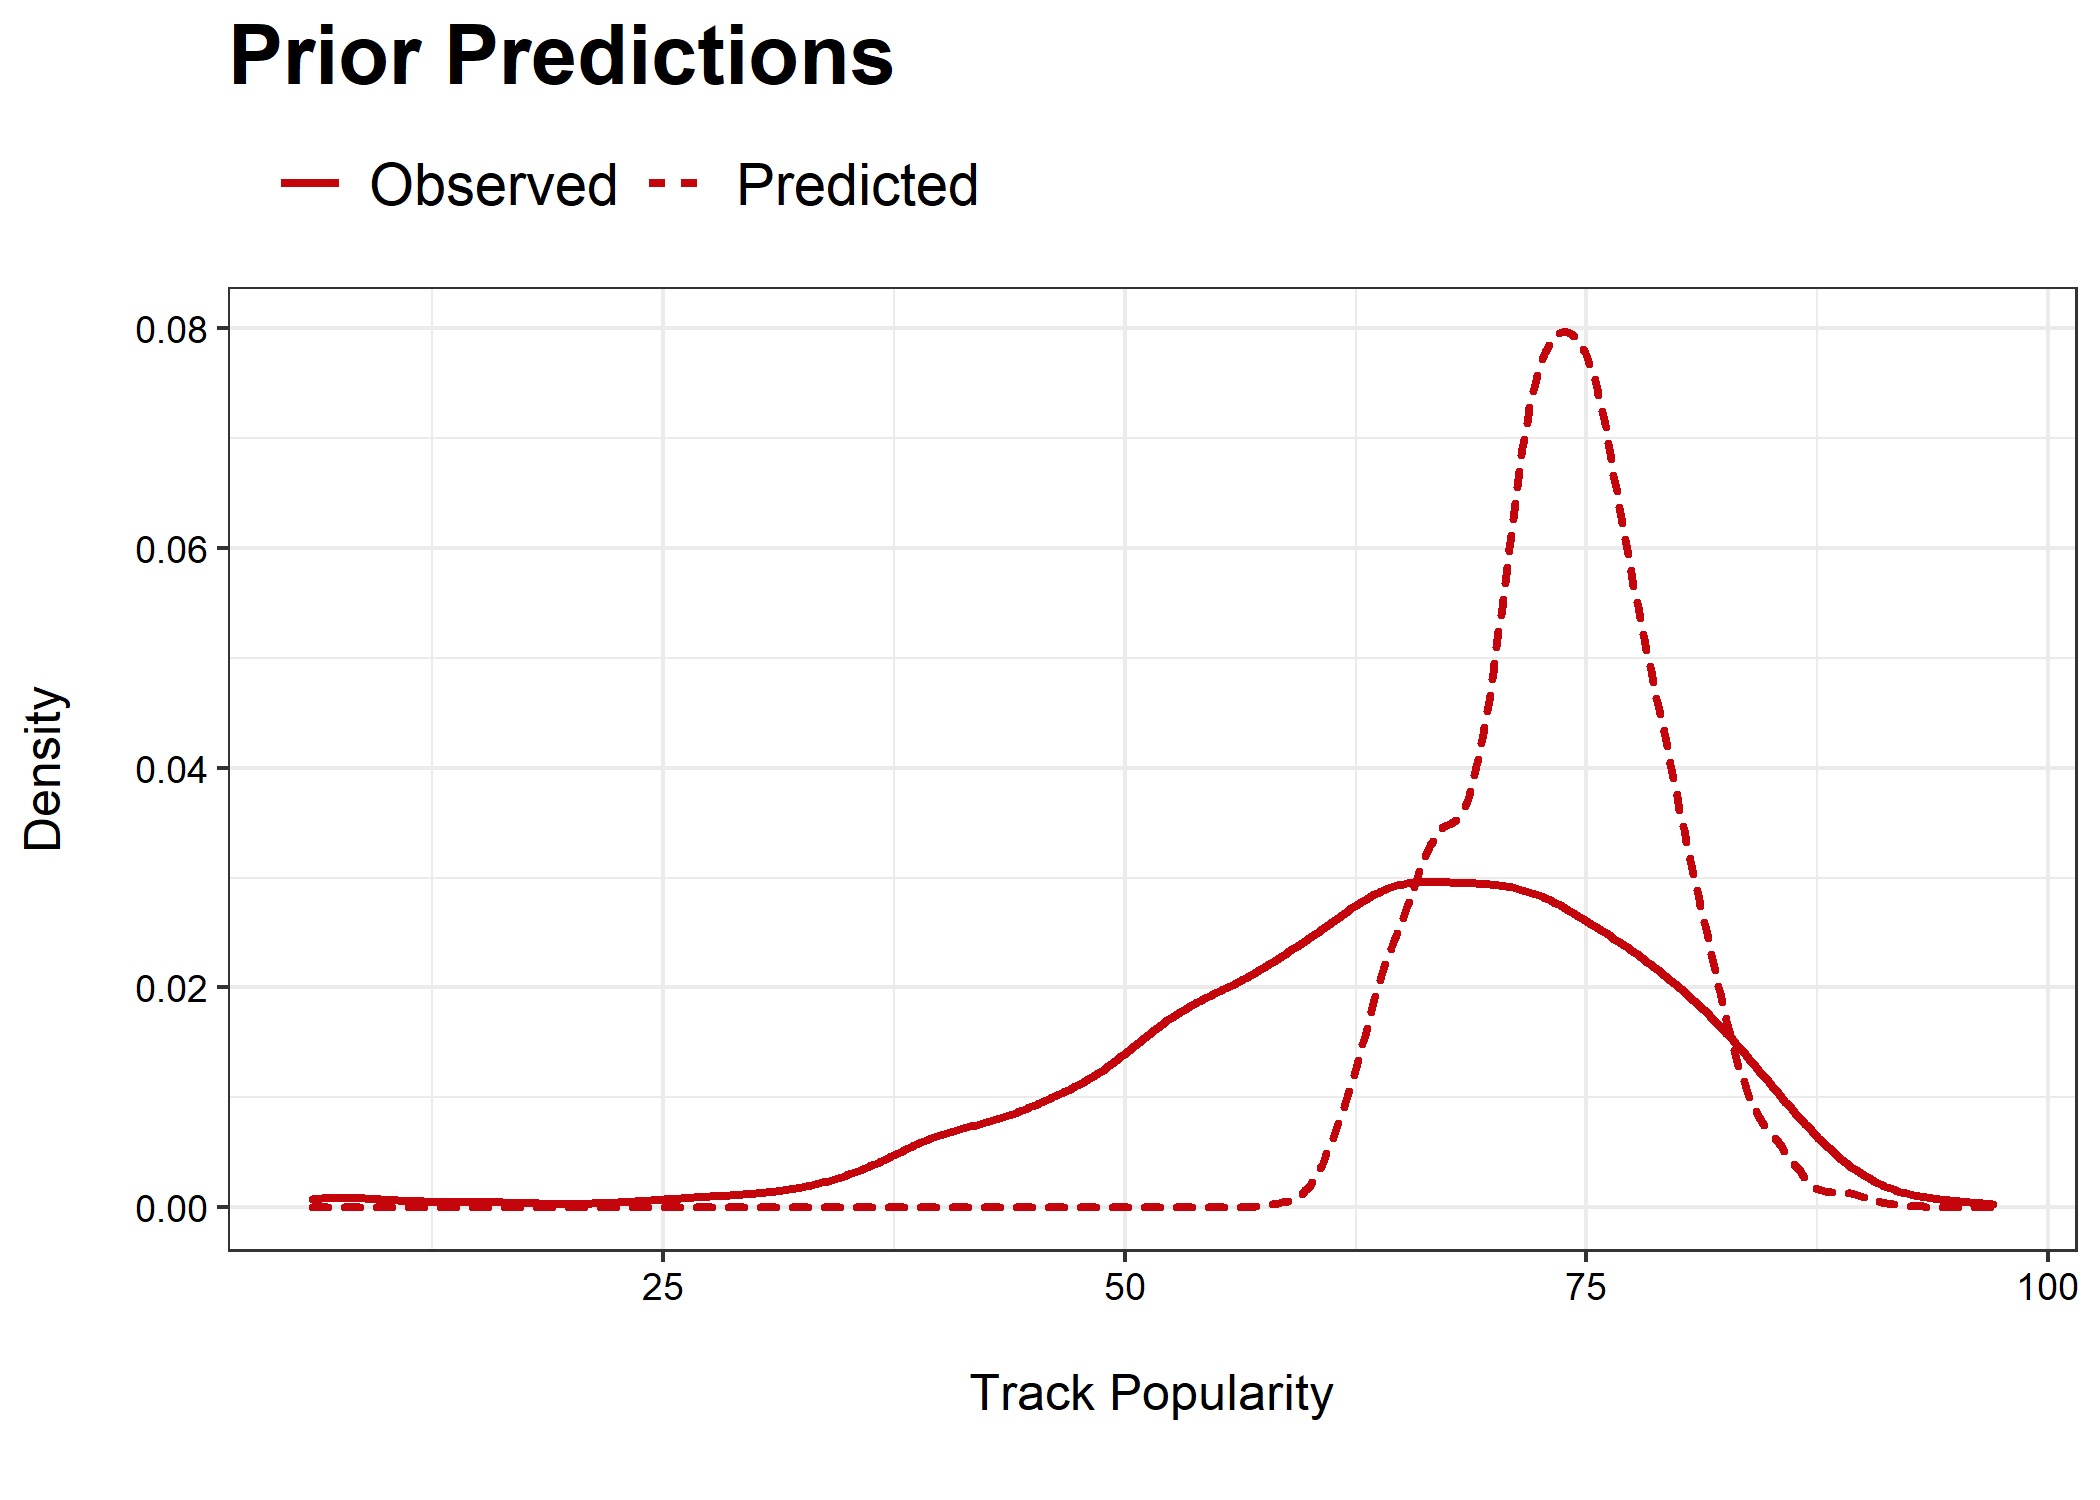
\includegraphics[width = \textwidth]{prior_predictions.png}
\caption{}
\label{fig:prior}
\end{subfigure}
\begin{subfigure}[b]{0.5\textwidth}
\centering
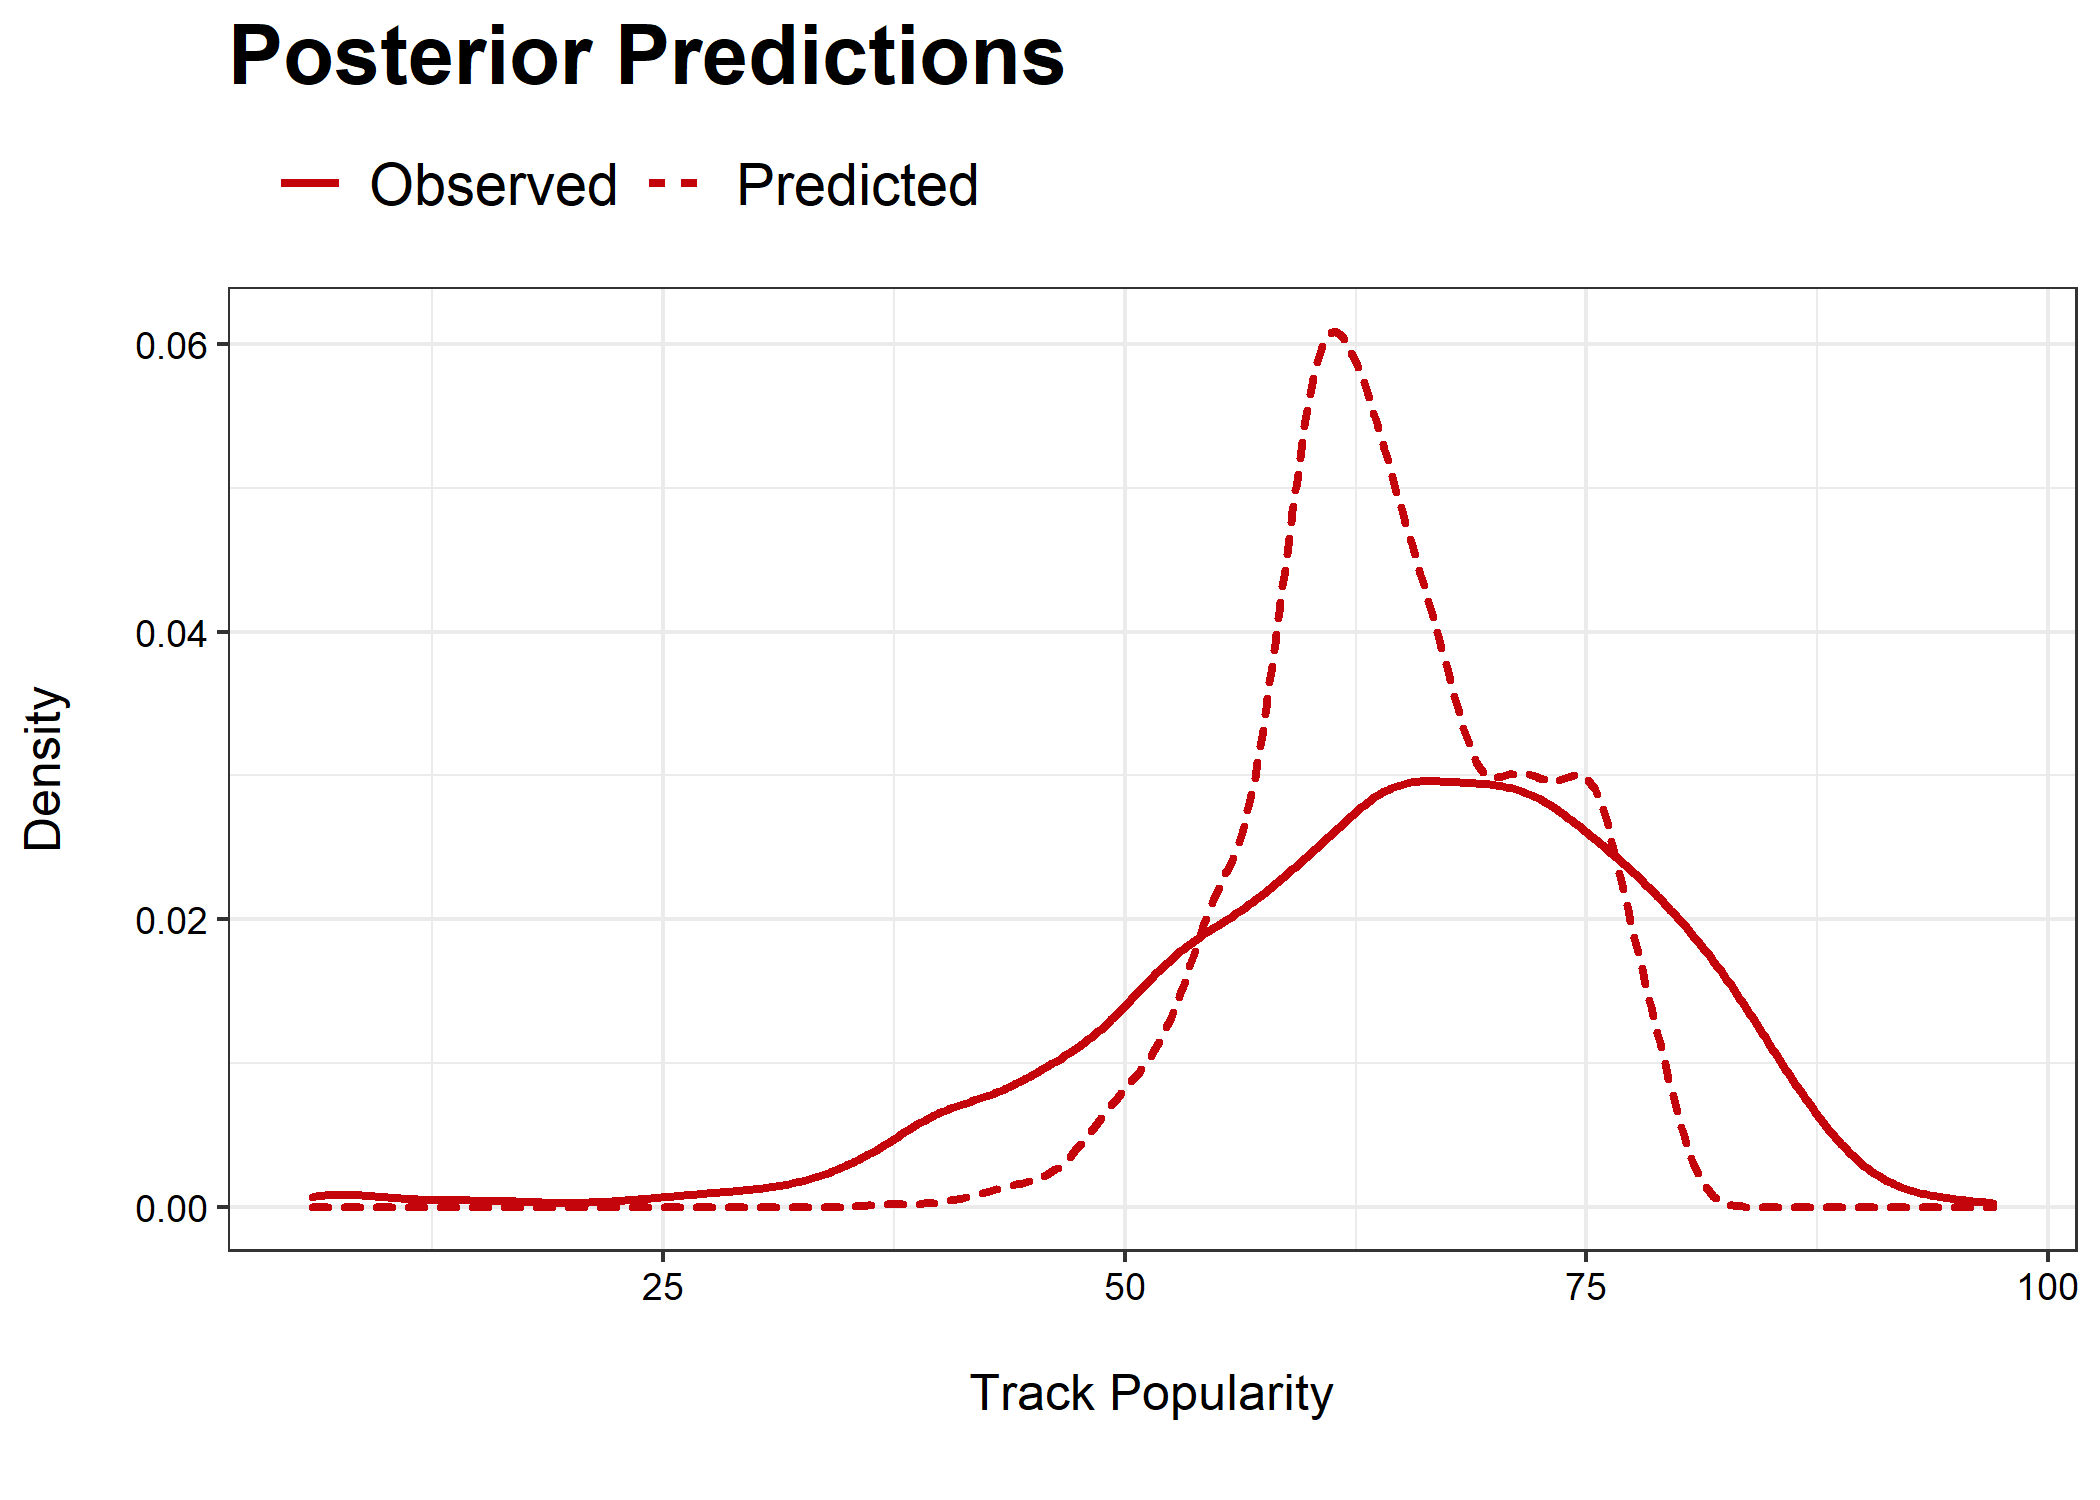
\includegraphics[width = \textwidth]{post_predictions.png}
\caption{}
\label{fig:post}
\end{subfigure}
\caption{Prior vs Posterior prediction means. The prior distribution placed almost all density near 75. The posterior pulls the prior leftward to better reflect the observed density, though very little density is placed near very low or very high values of popularity.}
\end{figure}

The negligible density around small values of popularity for the posterior predictive distribution is reflected in the residual vs fitted figure below, where we see that the model systemically over-predicts songs with low popularity:

\begin{figure}[H] % H forces the figure to appear in this location, h! tries really hard to do the same thing
\centering
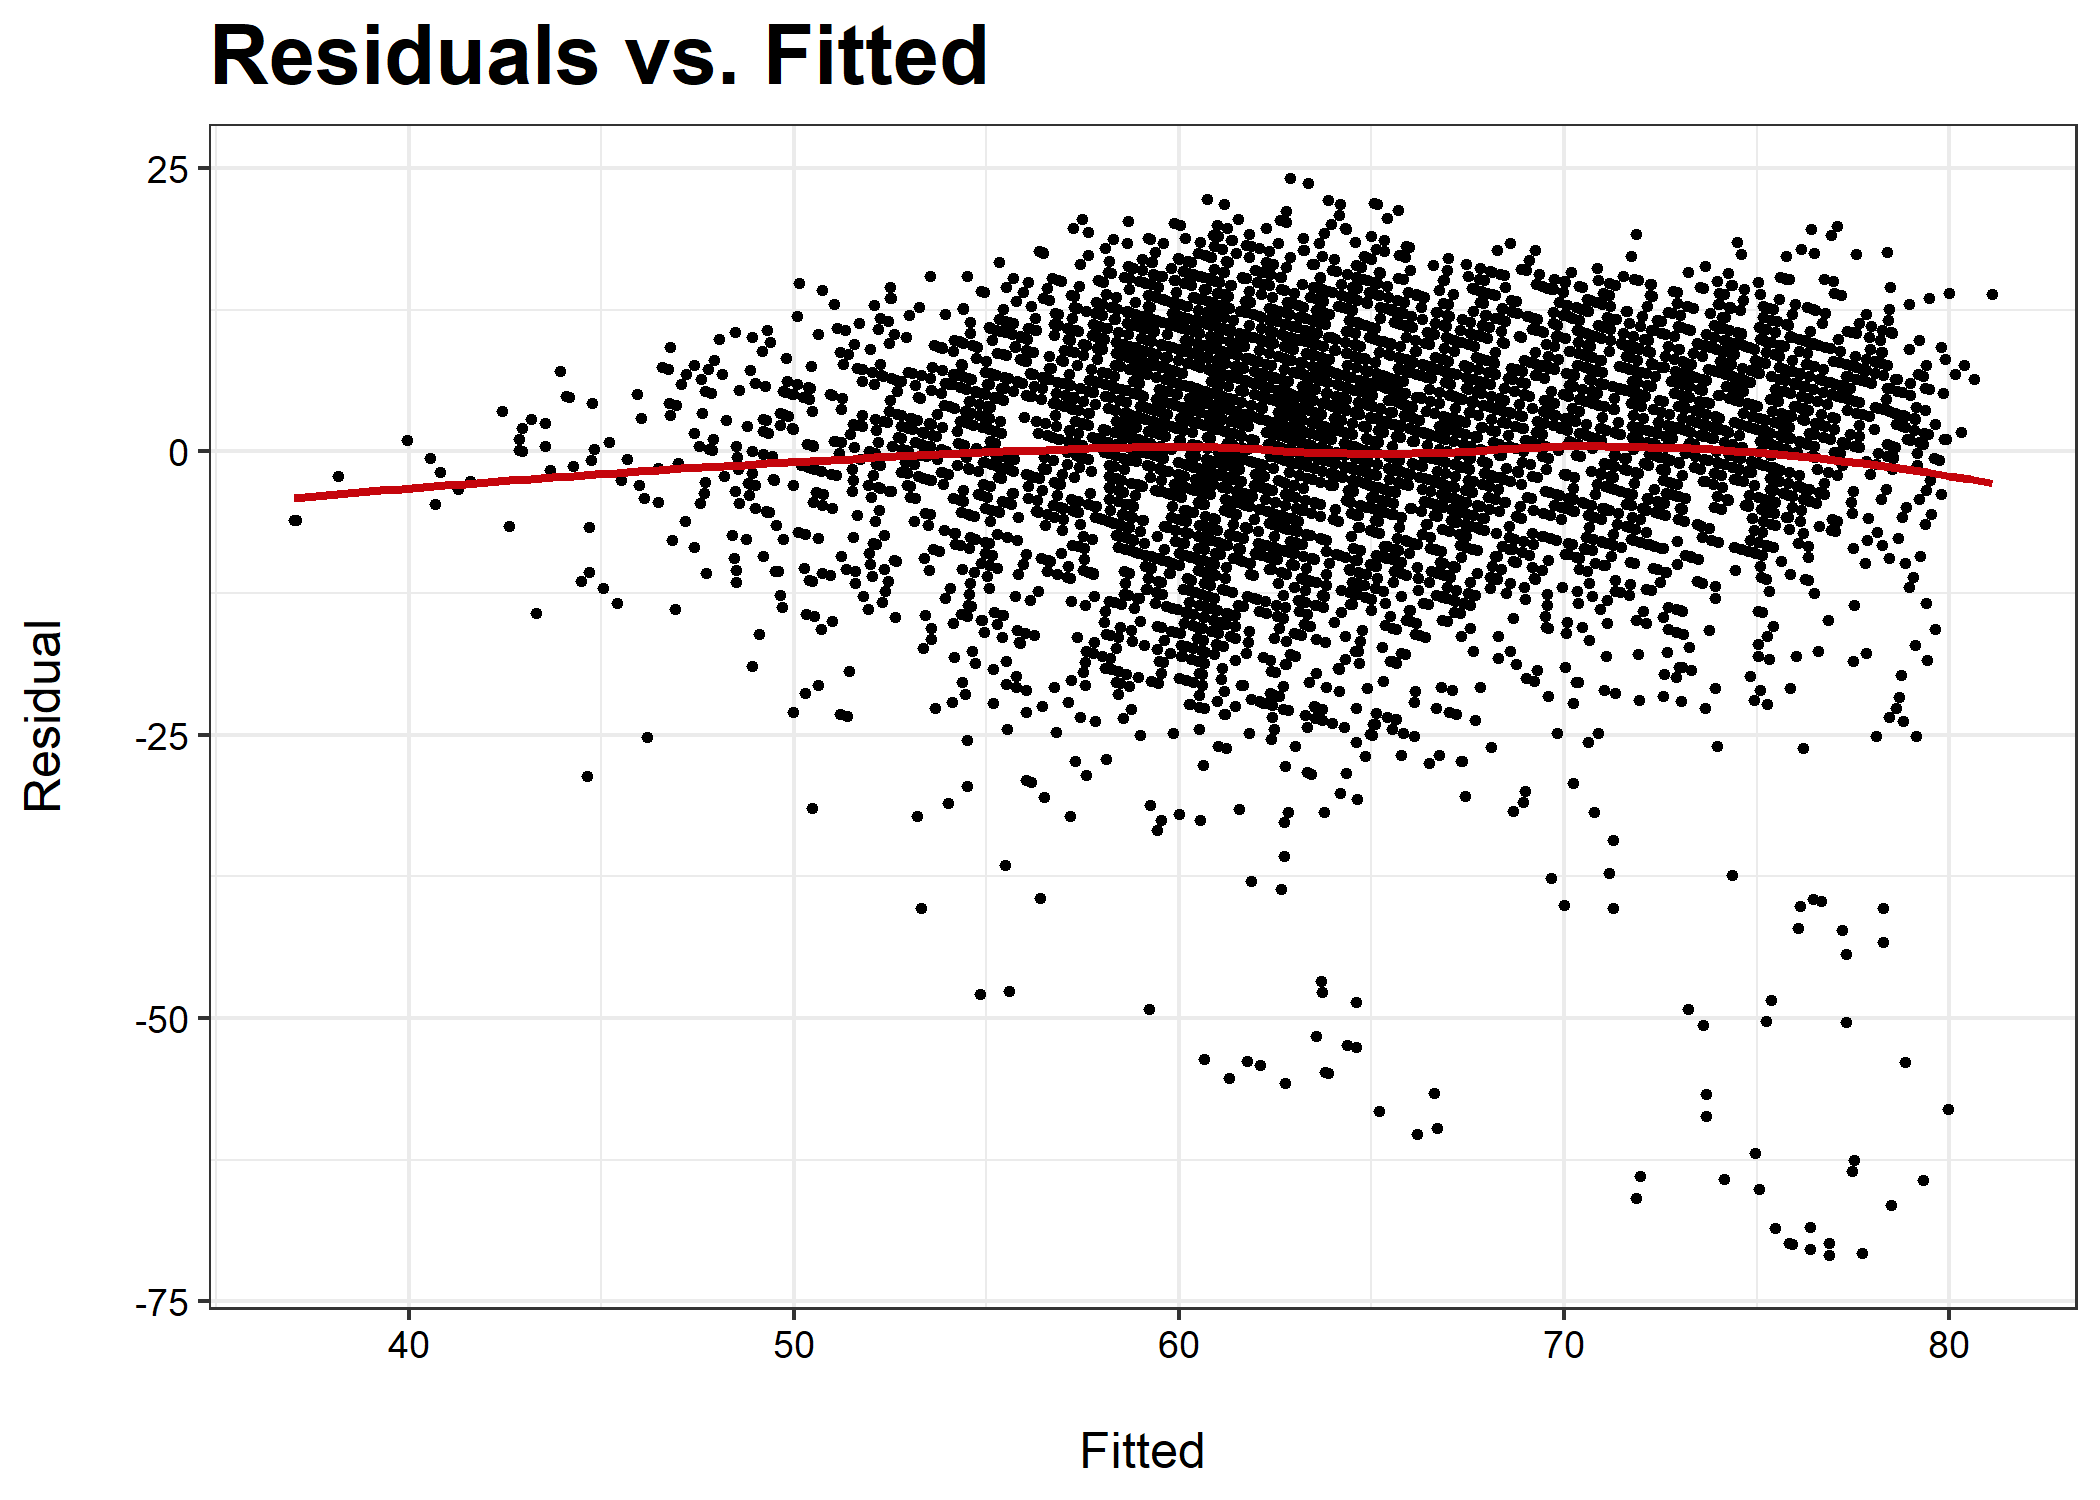
\includegraphics[width=0.7\textwidth]{residuals.png} % no need to specify a file extension & pay attention to scaling by width!
\caption{Residuals vs Fitted. Fitted values correspond to posterior means for each posterior predictive distribution.}
\label{fig:residuals} % useful for hyperref'ing later
\end{figure}

Despite the indication of weak predictive performance, it's still of interest to assess which predictors are most influential. 

\begin{figure}[H] % H forces the figure to appear in this location, h! tries really hard to do the same thing
\centering
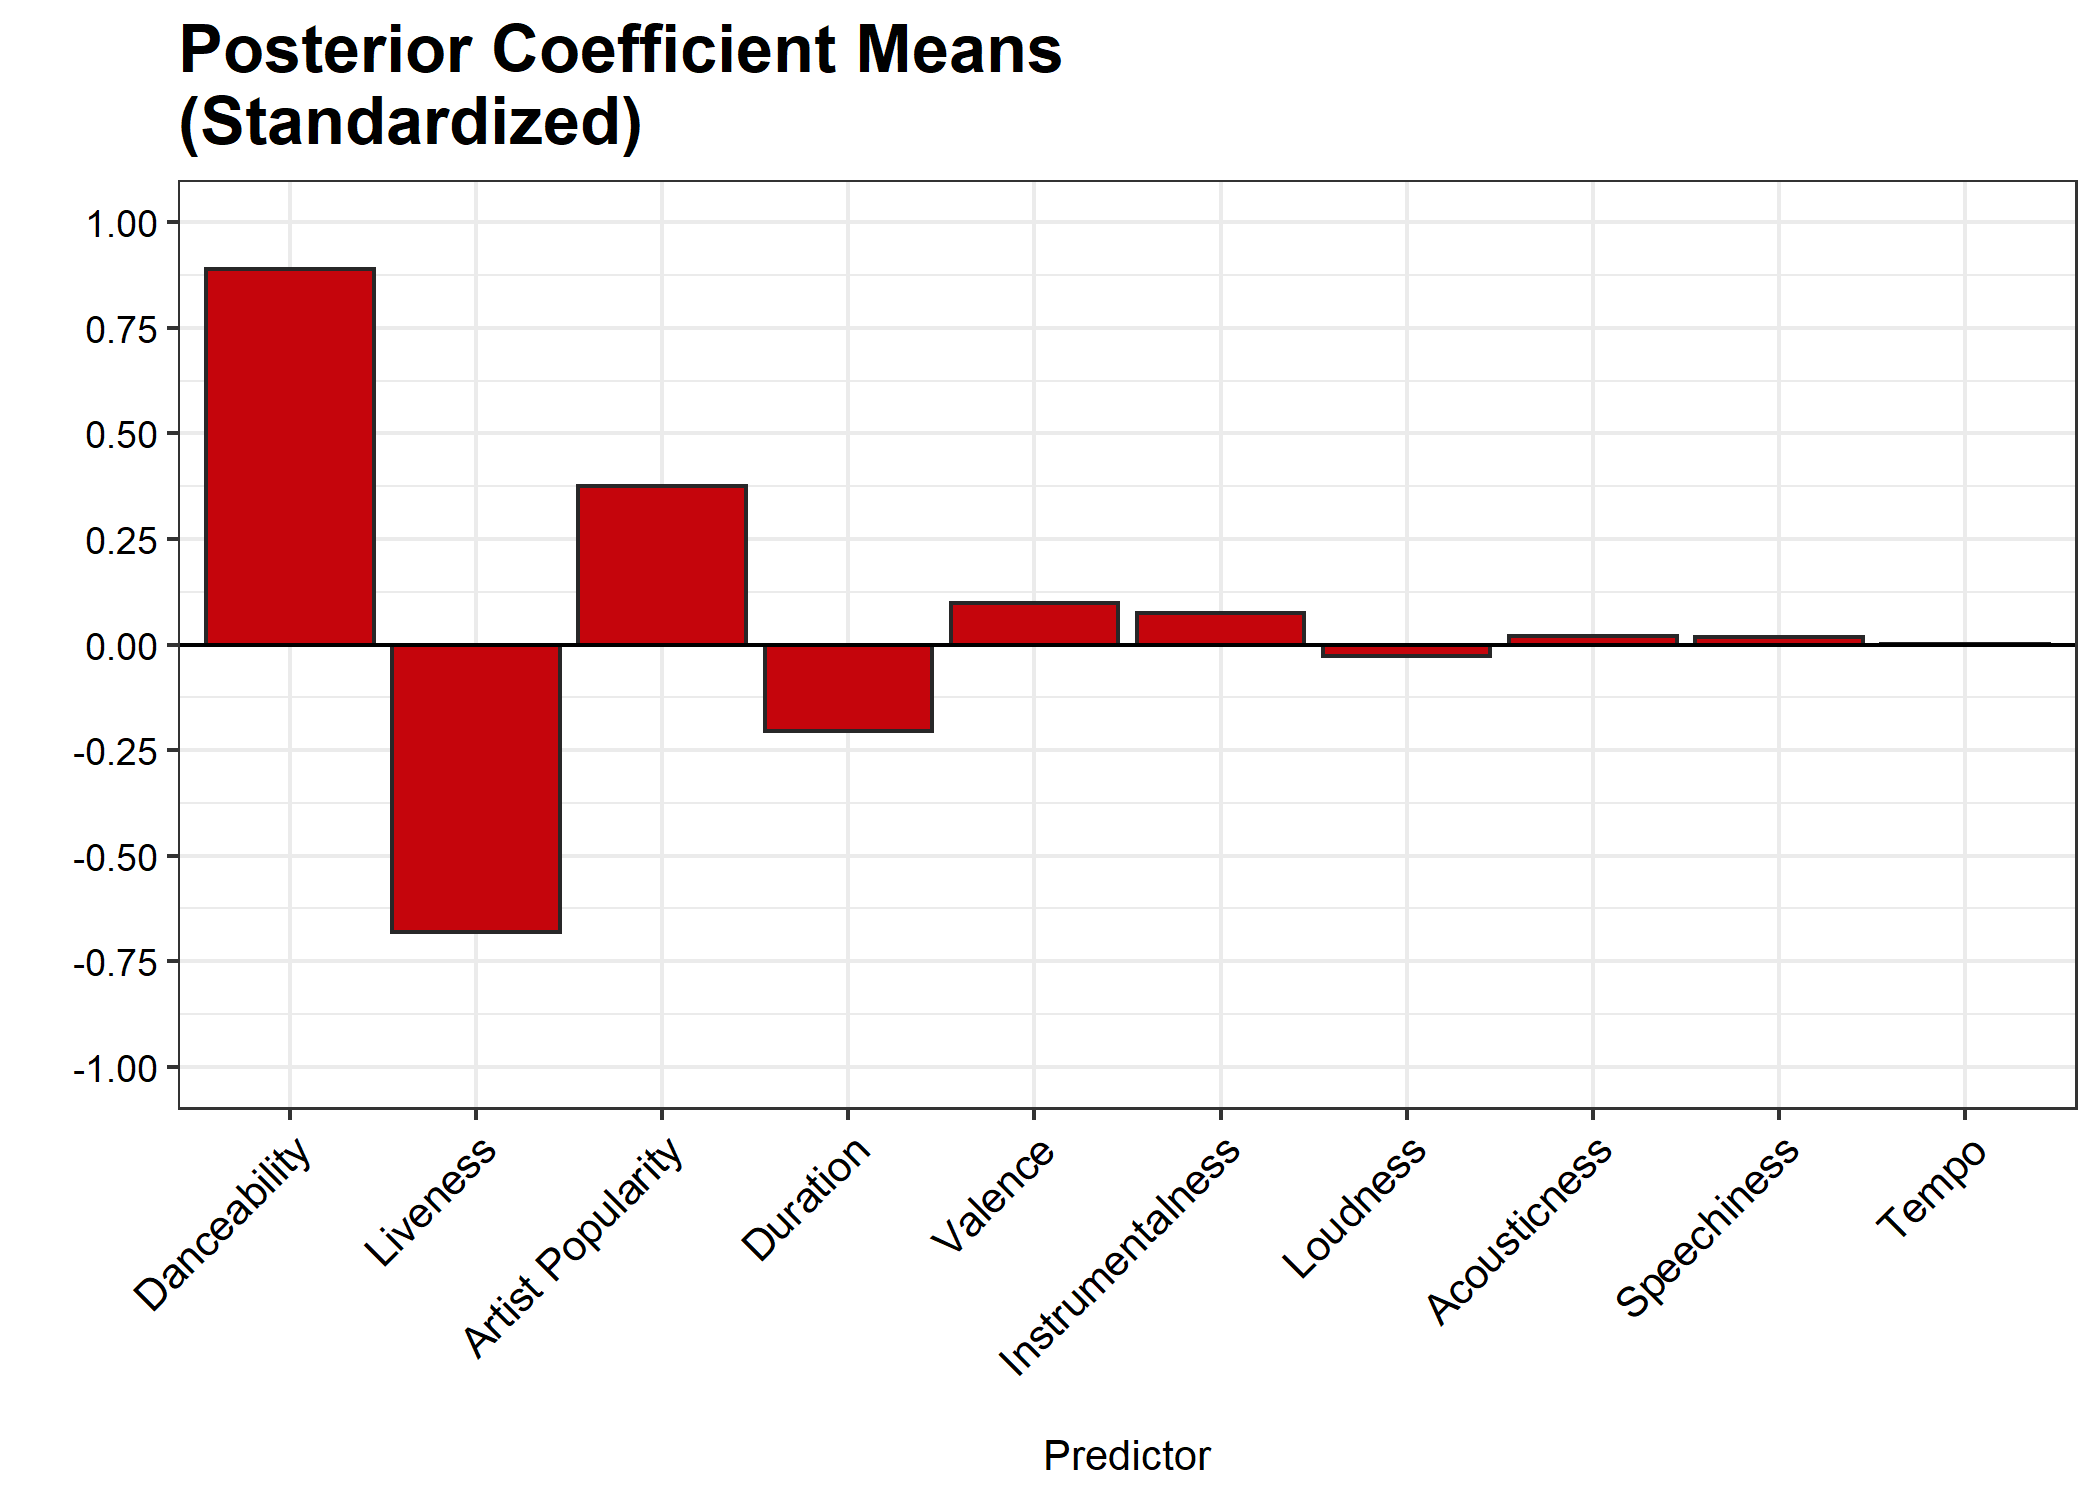
\includegraphics[width=0.7\textwidth]{standardized_coeffs.png} % no need to specify a file extension & pay attention to scaling by width!
\caption{Standardized posterior coefficient means. The data suggest that danceability has largest effect on popularity.}
\label{fig:standardized_coefs} % useful for hyperref'ing later
\end{figure}

We see that danceability appears most predictive of popularity---popular songs will typically leverage a pronounced, predictable beat with minimal rhythmic fluctuation. 

A hierarchical model with variable intercepts and slopes was used under the assumption that the effect of each predictor on popularity may vary by decade. To verify this assumption, we can plot the posterior distribution for each predictor. We find that for some predictors the effect does indeed vary by decade; for others, however, it does not.

\begin{figure}[H]
\begin{subfigure}[b]{0.5\textwidth}
\centering
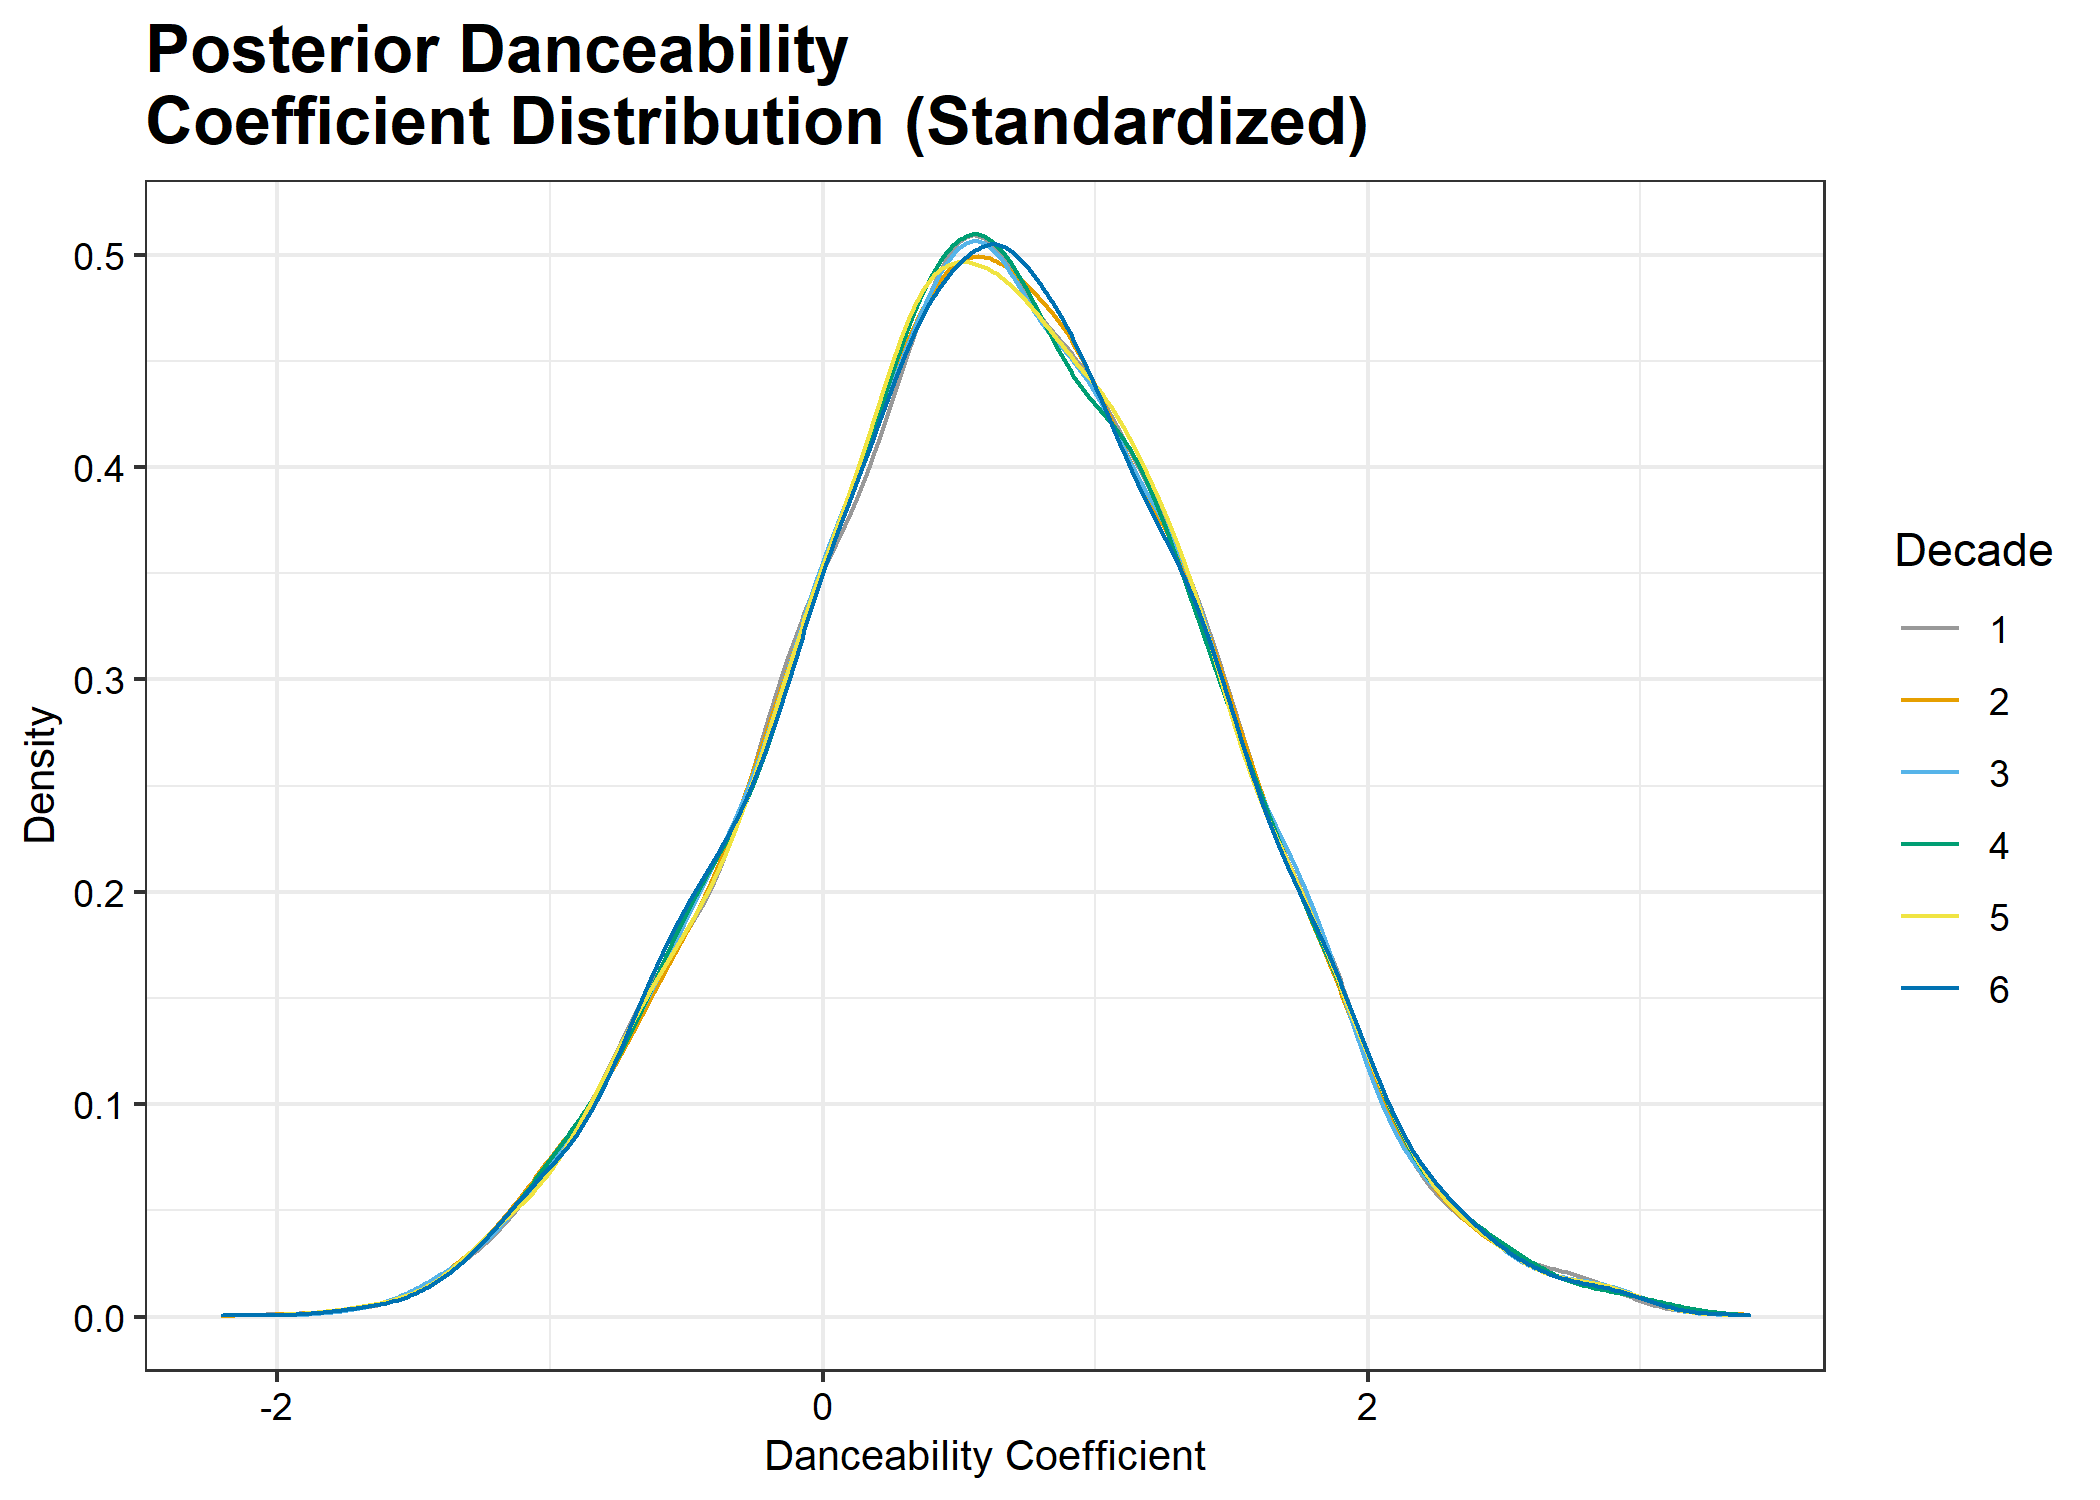
\includegraphics[width = \textwidth]{danceabiltiy_dist.png}
\caption{}
\label{fig:prior}
\end{subfigure}
\begin{subfigure}[b]{0.5\textwidth}
\centering
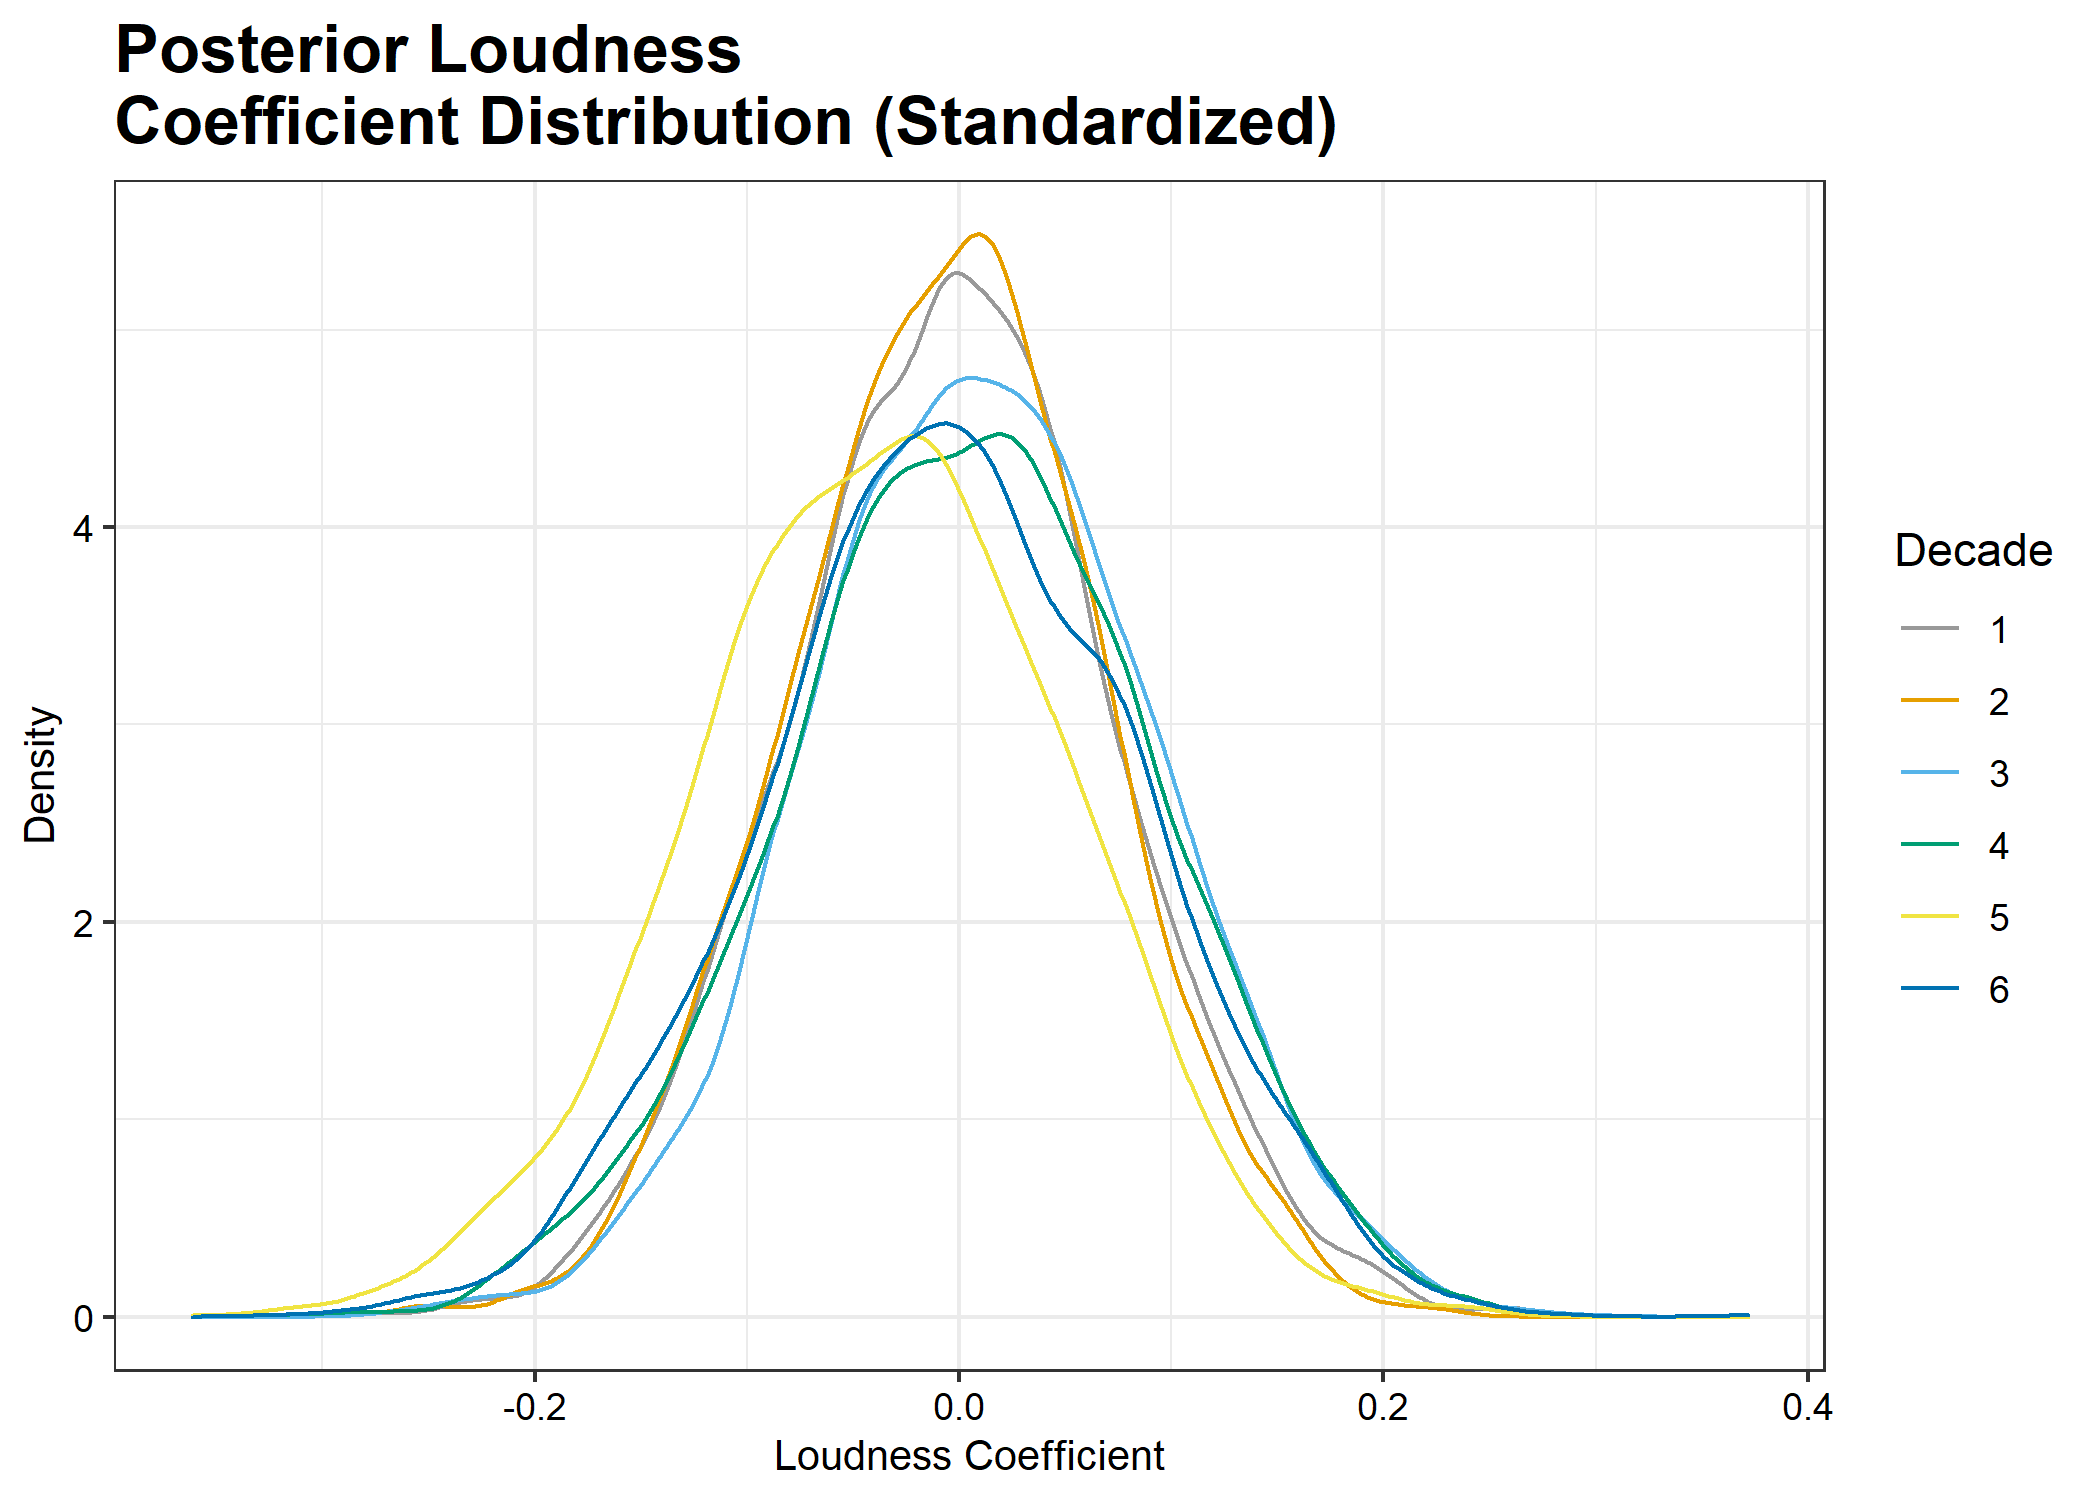
\includegraphics[width = \textwidth]{loudness_dist.png}
\caption{}
\label{fig:post}
\end{subfigure}
\caption{Posterior distributions of danceability and loudness coefficients. The effect of danceability does not vary much at all by decade, whereas the effect of loudness does vary by decade (albeit slightly). }
\end{figure}

\section{Discussion}
This analysis has shown that Spotify's audio features are weakly predictive of song popularity. Our collective perception of music is complicated. In some sense, it's not particularly surprising that popularity resists simplicity---a mere 10 predictors is generally insufficient for predicting popularity with confidence. That being said, the audio features that were considered do explain some variability in popularity, with the model suggesting danceability is most predictive.  

Indeed, there are other (unconsidered) features that may be important: 
\begin{itemize}
  \item Lyrical sentiment. The valence feature considers musical sentiment, but lyrical sentiment  may also be predictive of popularity.
  \item Marketing. Songs that are marketed heavily will, of course, likely rise in popularity.
  \item The TikTok Effect. Songs that circulate on TikTok tend to grow in popularity\footnote{\href{https://www.businessinsider.com/how-tiktok-is-changing-the-music-industry-marketing-discovery-2021-7}{https://www.businessinsider.com/how-tiktok-is-changing-the-music-industry-marketing-discovery-2021-7}}. How can we measure a song's ability to resonate with TikTok's primary audience?
  \item Seasonality. Songs that release during (or immediately before) summer may see increased popularity.
\end{itemize}

\end{document}
